% Soubory musí být v kódování, které je nastaveno v příkazu \usepackage[...]{inputenc}

\documentclass[%        Základní nastavení
%  draft,    				  % Testovací překlad
  11pt,       				% Velikost základního písma je 12 bodů
  a4paper,    				% Formát papíru je A4
  oneside,      			% Jednostranný tisk
  %twoside,      			% Dvoustranný tisk (kapitoly a další důležité části tedy začínají na lichých stranách)
	unicode,						% Záložky a metainformace ve výsledném  PDF budou v kódování unicode
]{report}				    	% Dokument třídy 'zpráva', vhodná pro sazbu závěrečných prací s kapitolami

\usepackage[utf8]		  %	Kódování zdrojových souborů je UTF-8
	{inputenc}					% Balíček pro nastavení kódování zdrojových souborů

\usepackage[				% Nastavení geometrie stránky
	bindingoffset=10mm,		% Hřbet pro vazbu
	hmargin={25mm,18mm},	% Vnitřní a vnější okraj
  %hmargin={25mm,25mm},	% Vnitřní a vnější okraj
	%vmargin={25mm,34mm},	% Horní a dolní okraj
  vmargin={20mm,25mm},	% Horní a dolní okraj
	footskip=15mm,			  % Velikost zápatí
	nohead,					      % Bez záhlaví
	marginparsep=2mm,		  % Vzdálenost marginálií
	marginparwidth=18mm,	% Šířka marginálií
]{geometry}

\setcounter{tocdepth}{3}

\usepackage{sectsty}
	%přetypuje nadpisy všech úrovní na bezpatkové, kromě \chapter, která je přenastavena zvlášť v thesis.sty
	\allsectionsfont{\sffamily}

\usepackage{graphicx} % Balíček 'graphicx' pro vkládání obrázků
											% Nutné pro vložení logotypů školy a fakulty

\usepackage[          % Balíček 'acronym' pro sazby zkratek a symbolů
	nohyperlinks				% Nebudou tvořeny hypertextové odkazy do seznamu zkratek
]{acronym}						
											% Nutné pro použití prostředí 'acronym' balíčku 'thesis'

\usepackage[
	breaklinks=true,		% Hypertextové odkazy mohou obsahovat zalomení řádku
	hypertexnames=false % Názvy hypertext. odkazů budou tvořeny nezávisle na názvech TeXu
]{hyperref}						% Balíček 'hyperref' pro sazbu hypertextových odkazů
											% Nutné pro použití příkazu 'pdfsettings' balíčku 'thesis'

\usepackage{pdfpages} % Balíček umožňující vkládat stránky z PDF souborů
                      % Nutné při vkládání titulních listů a zadání přímo
                      % ve formátu PDF z informačního systému

\usepackage{enumitem} % Balíček pro nastavení mezerování v odrážkách
  \setlist{topsep=0pt,partopsep=0pt,noitemsep} % konkrétní nastavení

\usepackage{cmap} 		% Balíček cmap zajišťuje, že PDF vytvořené `pdflatexem' je
											% plně "prohledávatelné" a "kopírovatelné"

%\usepackage{upgreek}	% Balíček pro sazbu stojatých řeckých písmem
											%% např. stojaté pí: \uppi
											%% např. stojaté mí: \upmu (použitelné třeba v mikrometrech)
											%% pozor, grafická nekompatibilita s fonty typu Computer Modern!
                      
%\usepackage{amsmath} %balíček pro sabu náročnější matematiky                 

\usepackage{dirtree}	% sazba adresářové struktury
                      % vhodné pro prezentaci obsahu elektronické přílohy (např. CD)
                    
\usepackage{indentfirst}
\usepackage{pdflscape}

\usepackage[formats]{listings}	% Balíček pro sazbu zdrojových textů
\lstset{              % nastavení
%	Definice jazyka použitého ve výpisech
%    language=[LaTeX]{TeX},	% LaTeX
%	language={Matlab},		% Matlab
	language={C},           % jazyk C
    basicstyle=\ttfamily,	% definice základního stylu písma
    tabsize=2,			% definice velikosti tabulátoru
    inputencoding=utf8,         % pro soubory uložené v kódování UTF-8
		columns=fixed,  %fixed nebo flexible,
		fontadjust=true %licovani sloupcu
    extendedchars=true,
    literate=%  definice symbolů s diakritikou
    {á}{{\'a}}1
    {č}{{\v{c}}}1
    {ď}{{\v{d}}}1
    {é}{{\'e}}1
    {ě}{{\v{e}}}1
    {í}{{\'i}}1
    {ň}{{\v{n}}}1
    {ó}{{\'o}}1
    {ř}{{\v{r}}}1
    {š}{{\v{s}}}1
    {ť}{{\v{t}}}1
    {ú}{{\'u}}1
    {ů}{{\r{u}}}1
    {ý}{{\'y}}1
    {ž}{{\v{z}}}1
    {Á}{{\'A}}1
    {Č}{{\v{C}}}1
    {Ď}{{\v{D}}}1
    {É}{{\'E}}1
    {Ě}{{\v{E}}}1
    {Í}{{\'I}}1
    {Ň}{{\v{N}}}1
    {Ó}{{\'O}}1
    {Ř}{{\v{R}}}1
    {Š}{{\v{S}}}1
    {Ť}{{\v{T}}}1
    {Ú}{{\'U}}1
    {Ů}{{\r{U}}}1
    {Ý}{{\'Y}}1
    {Ž}{{\v{Z}}}1
}

%%%%%%%%%%%%%%%%%%%%%%%%%%%%%%%%%%%%%%%%%%%%%%%%%%%%%%%%%%%%%%%%%
%%%%%%      Definice informací o dokumentu             %%%%%%%%%%
%%%%%%%%%%%%%%%%%%%%%%%%%%%%%%%%%%%%%%%%%%%%%%%%%%%%%%%%%%%%%%%%%

% V tomto souboru se nastavují téměř veškeré informace, proměnné mezi studenty:
% jméno, název práce, pohlaví atd.
% Tento soubor je SDÍLENÝ mezi textem práce a prezentací k obhajobě -- netřeba něco nastavovat na dvou místech.

\usepackage[
%%% Z následujících voleb jazyka lze použít pouze jednu
  czech-english,		% originální jazyk je čeština, překlad je anglicky (výchozí)
  %english-czech,	% originální jazyk je angličtina, překlad je česky
  %slovak-english,	% originální jazyk je slovenština, překlad je anglicky
  %english-slovak,	% originální jazyk je angličtina, překlad je slovensky
%
%%% Z následujících voleb typu práce lze použít pouze jednu
  %semestral,		  % semestrální práce (nesází se abstrakty, prohlášení, poděkování) (výchozí)
  %bachelor,			%	bakalářská práce
  master,			  % diplomová práce
  %treatise,			% pojednání o disertační práci
  %doctoral,			% disertační práce
%
%%% Z následujících voleb zarovnání objektů lze použít pouze jednu
%  left,				  % rovnice a popisky plovoucích objektů budou zarovnány vlevo
	center,			    % rovnice a popisky plovoucích objektů budou zarovnány na střed (vychozi)
%
]{thesis}   % Balíček pro sazbu studentských prací


%%% Jméno a příjmení autora ve tvaru
%  [tituly před jménem]{Křestní}{Příjmení}[tituly za jménem]
% Pokud osoba nemá titul před/za jménem, smažte celý řetězec '[...]'
\author[Bc.]{Filip}{Paul}

%%% Identifikační číslo autora (VUT ID)
\butid{211 538}

%%% Pohlaví autora/autorky
% (nepoužije se ve variantě english-czech ani english-slovak)
% Číselná hodnota: 1...žena, 0...muž
\gender{0}

%%% Jméno a příjmení vedoucího/školitele včetně titulů
%  [tituly před jménem]{Křestní}{Příjmení}[tituly za jménem]
% Pokud osoba nemá titul před/za jménem, smažte celý řetězec '[...]'
\advisor[prof.\ Dr.\ Ing.]{Zdeněk}{Kolka}

%%% Jméno a příjmení oponenta včetně titulů
%  [tituly před jménem]{Křestní}{Příjmení}[tituly za jménem]
% Pokud osoba nemá titul před/za jménem, smažte celý řetězec '[...]'
% Nastavení oponenta se uplatní pouze v prezentaci k obhajobě;
% v případě, že nechcete, aby se na titulním snímku prezentace zobrazoval oponent, pouze příkaz zakomentujte;
% u obhajoby semestrální práce se oponent nezobrazuje (jelikož neexistuje)
% U dizertační práce jsou typicky dva až tři oponenti. Pokud je chcete mít na titulním slajdu, prosím ručně odkomentujte a upravte jejich jména v definici "VUT title page" v souboru thesis.sty.
\opponent[doc.\ Mgr.]{Křestní}{Příjmení}[Ph.D.]

%%% Název práce
%  Parametr ve složených závorkách {} je název v originálním jazyce,
%  parametr v hranatých závorkách [] je překlad (podle toho jaký je originální jazyk).
%  V případě, že název Vaší práce je dlouhý a nevleze se celý do zápatí prezentace, použijte příkaz
%  \def\insertshorttitle{Zkác.\ náz.\ práce}
%  kde jako parametr vyplníte zkrácený název. Pokud nechcete zkracovat název, budete muset předefinovat,
%  jak se vytváří patička slidu. Viz odkaz: https://bit.ly/3EJTp5A
\title[Title of Student's Thesis]{Výrobní tester}

%%% Označení oboru studia
%  Parametr ve složených závorkách {} je název oboru v originálním jazyce,
%  parametr v hranatých závorkách [] je překlad
\specialization[Teleinformatics]{Teleinformatika}

%%% Označení ústavu
%  Parametr ve složených závorkách {} je název ústavu v originálním jazyce,
%  parametr v hranatých závorkách [] je překlad
%\department[Department of Control and Instrumentation]{Ústav automatizace a měřicí techniky}
%\department[Department of Biomedical Engineering]{Ústav biomedicínského inženýrství}
%\department[Department of Electrical Power Engineering]{Ústav elektroenergetiky}
%\department[Department of Electrical and Electronic Technology]{Ústav elektrotechnologie}
%\department[Department of Physics]{Ústav fyziky}
%\department[Department of Foreign Languages]{Ústav jazyků}
%\department[Department of Mathematics]{Ústav matematiky}
%\department[Department of Microelectronics]{Ústav mikroelektroniky}
\department[Department of Radio Electronics]{Ústav radioelektroniky}
%\department[Department of Theoretical and Experimental Electrical Engineering]{Ústav teoretické a experimentální elektrotechniky}
%\department[Department of Telecommunications]{Ústav telekomunikací}
%\department[Department of Power Electrical and Electronic Engineering]{Ústav výkonové elektrotechniky a elektroniky}

%%% Označení fakulty
%  Parametr ve složených závorkách {} je název fakulty v originálním jazyce,
%  parametr v hranatých závorkách [] je překlad
%\faculty[Faculty of Architecture]{Fakulta architektury}
\faculty[Faculty of Electrical Engineering and~Communication]{Fakulta elektrotechniky a~komunikačních technologií}
%\faculty[Faculty of Chemistry]{Fakulta chemická}
%\faculty[Faculty of Information Technology]{Fakulta informačních technologií}
%\faculty[Faculty of Business and Management]{Fakulta podnikatelská}
%\faculty[Faculty of Civil Engineering]{Fakulta stavební}
%\faculty[Faculty of Mechanical Engineering]{Fakulta strojního inženýrství}
%\faculty[Faculty of Fine Arts]{Fakulta výtvarných umění}
%
%Nastavení logotypu (v hranatych zavorkach zkracene logo, ve slozenych plne):
\facultylogo[logo/FEKT_zkratka_barevne_PANTONE_CZ]{logo/FEKT_zkratka_barevne_PANTONE_CZ}

%%% Rok odevzdání práce
\graduateyear{2023}
%%% Akademický rok odevzdání práce
\academicyear{2022/23}

%%% Datum obhajoby (uplatní se pouze v prezentaci k obhajobě)
\date{6.\,6.\,2023} 

%%% Místo obhajoby
% Na titulních stránkách bude automaticky vysázeno VELKÝMI písmeny (pokud tyto stránky sází šablona)
\city{Brno}

%%% Abstrakt
\abstract[%
The diploma thesis deals with the design and implementation of a device,
which is used to verify the internal electrical wiring of ICT testers.
Wiring is verified by measuring the resistance between individual test points.
ICT testers can contain thousands of connections. The device should be able to identify wiring errors,
inform the operator about the error and propose a relevant solution.

]{%
Diplomová práce se zabývá návrhem a realizací zařízení, které slouží k ověření 
správnosti vnitřního elektrického zapojení ICT testerů. Správnost zapojení
je ověřována měřením odporu mezi jednotlivýmy testovacími body.
ICT testery mohou obsahovat řádově tisíce propojení. Navrhované zařízení by mělo být
schopno identifikovat chyby propojení a následně navrhnout vhodné řešení.

}

%%% Klíčová slova
\keywrds[%
In-Circuit Testing (ICT), Fixture, Testpoint, Test probes, End Of Line (EOL).
]{%
In-Circuit Testing (ICT), Fixture, Testovací body, Testovací jehly, End Of Line (EOL).
}

%%% Poděkování
\acknowledgement{%
Rád bych poděkoval vedoucímu diplomové práce
panu Prof. Dr. Ing. Zdeňku Kolkovi za odborné vedení,
konzultace, trpělivost a~podnětné návrhy k~práci.
}%  % do tohoto souboru doplňte údaje o sobě, druhu práce, názvu...

%%%%%%%%%%%%%%%%%%%%%%%%%%%%%%%%%%%%%%%%%%%%%%%%%%%%%%%%%%%%%%%%%%%%%%%%

%%%%%%%%%%%%%%%%%%%%%%%%%%%%%%%%%%%%%%%%%%%%%%%%%%%%%%%%%%%%%%%%%%%%%%%%
%%%%%%     Nastavení polí ve Vlastnostech dokumentu PDF      %%%%%%%%%%%
%%%%%%%%%%%%%%%%%%%%%%%%%%%%%%%%%%%%%%%%%%%%%%%%%%%%%%%%%%%%%%%%%%%%%%%%
%% Při načteném balíčku 'hyperref' lze použít příkaz '\pdfsettings':
\pdfsettings
%  Nastavení polí je možné provést také ručně příkazem:
%\hypersetup{
%  pdftitle={Název studentské práce},    	% Pole 'Document Title'
%  pdfauthor={Autor studenstké práce},   	% Pole 'Author'
%  pdfsubject={Typ práce}, 						  	% Pole 'Subject'
%  pdfkeywords={Klíčová slova}           	% Pole 'Keywords'
%}
%%%%%%%%%%%%%%%%%%%%%%%%%%%%%%%%%%%%%%%%%%%%%%%%%%%%%%%%%%%%%%%%%%%%%%%
\pdfmapfile{=vafle.map}

%%%%%%%%%%%%%%%%%%%%%%%%%%%%%%%%%%%%%%%%%%%%%%%%%%%%%%%%%%%%%%%%%%%%%%%
%%%%%%%%%%%       Začátek dokumentu               %%%%%%%%%%%%%%%%%%%%%
%%%%%%%%%%%%%%%%%%%%%%%%%%%%%%%%%%%%%%%%%%%%%%%%%%%%%%%%%%%%%%%%%%%%%%%
\usepackage[hidelinks]{xurl}
\hypersetup{
    colorlinks,
    citecolor=black,
    filecolor=black,
    linkcolor=black,
    urlcolor=black
}
%\usepackage[hidelinks]{hyperref}

\begin{document}
\pagestyle{empty} %vypnutí číslování stránek

%%% Vložení desek -- od září 2021 na žádost fakulty nepoužíváno
%\includepdf[pages=1]%  buďto generovaných informačním systémem
  %{pdf/student-desky}% název souboru nesmí obsahovat mezery!
%%% NEBO vytvoření desek z balíčku
%%\makecover
%%%
%\oddpage % při dvojstranném tisku přidá prázdnou stránku
%% kazdopádně ale:
%\setcounter{page}{1} %resetovaní čítače stránek -- desky do číslování nezahrnujeme

%% Vložení titulního listu
\includepdf[pages=1]%    buďto generovaného informačním systémem
  {pdf/student-titulka}% název souboru nesmí obsahovat mezery!
%% NEBO vytvoření titulní stránky z balíčku
%\maketitle
%%
\oddpage  % při dvojstranném tisku se přidá prázdná stránka
   
%% Vložení zadání
\includepdf[pages=1]%   buďto generovaného informačním systémem
  {pdf/student-zadani}% název souboru nesmí obsahovat mezery!
%% NEBO lze vytvořit prázdný list příkazem ze šablony
%\patternpage{}%
%	{\sffamily\Huge\centering ZDE VLOŽIT LIST ZADÁNÍ}%
%	{\sffamily\centering Z~důvodu správného číslování stránek}
%%

\oddpage% při dvojstranném tisku se přidá prázdná stránka

%% Vysázení stránky s abstraktem
\makeabstract

% Vysázení stránky s rozšířeným abstraktem
% (pokud píšete práci v češtině či slovenštině, vložení rozšířeného abstraktu zrušte;
%  pro semestrální projekt také není potřeba rozšířený abstrakt uvádět)
%% Vysázení stránky s rozšířeným abstraktem
% (týká se pouze bc. a dp. prací psaných v angličtině, viz Směrnice rektora 72/2017)
\cleardoublepage
\noindent
{\large\sffamily\bfseries\MakeUppercase{Rozšířený abstrakt}}
\\
Výtah ze směrnice rektora 72/2017:\\
\emph{Bakalářská a diplomová práce předložená v angličtině musí obsahovat rozšířený abstrakt v češtině
nebo slovenštině (čl. 15). To se netýká studentů, kteří studují studijní program akreditovaný v
angličtině.}
(čl. 3, par. 7)\\
\emph{Nebude-li vnitřní normou stanoveno jinak, doporučuje se rozšířený abstrakt o rozsahu přibližně 3
normostrany, který bude obsahovat úvod, popis řešení a shrnutí a zhodnocení výsledků.}
(čl. 15, par. 5)

%%% Vysázení citace práce
\makecitation

%%% Vysázení prohlášení o samostatnosti
\makedeclaration

%%% Vysázení poděkování
%\makeacknowledgement

%%% Vysázení obsahu
\tableofcontents

%%% Vysázení seznamu obrázků
% (vynechejte, pokud máte dva nebo méně obrázků)
\listoffigures

%%% Vysázení seznamu tabulek
% (vynechejte, pokud máte dvě nebo méně tabulek)
%\listoftables

%%% Vysázení seznamu výpisů kódu
% (vynechejte, pokud máte dva nebo méně výpisů)
%\lstlistoflistings

\cleardoublepage\pagestyle{plain}   % zapnutí číslování stránek
%\setcounter{page}{1}

%Pro vkládání kapitol i příloh používejte raději \include než \input
%%% Vložení souboru 'text/uvod.tex' s úvodem
\chapter*{Úvod}
\phantomsection
\addcontentsline{toc}{chapter}{Úvod}

\indent Cílem diplomové práce je navrhnout zařízení,
které bude schopno ověřit správnost interního zapojení In Circuit Testing (ICT) testerů.
ICT tester slouží k odhalování výrobních chyb a programování Desek Plošných Spojů (DSP - dále
označováno jako PCB z anglického Printed Circuit Board)
pomocí připojení velkého množství testovacích jehel. Testovací jehly jsou připojovány do určených
míst na PCB, kde se následně provádí různé testy.\\

Diplomová práce je vypracována ve spolupráci s firmou Čevor inovation a.s.,
která se zabývá výrobou ICT testerů. Při výrobě těchto testerů vzniká potřeba kontroly správnosti zapojení fixture části.
Fixture část je označení pro zakládání (Obr. \ref{fig:ICT_tester}), je odlišná pro každé PCB a obsahuje řádově tisíce propojení.
Zařízení navrhované v této práci tak není ICT testerem samotným,
ale slouží právě k ověření správnosti interního zapojení fixture části ICT testeru.
Jedná se tedy o tester ICT testerů.\\

Ověření správnosti propojení se určuje odporem elektrické cesty.
Zařízení tedy musí být schopno měřit odpor mezi kterýmikoliv dvěma testovanými body.
Zároveň jsou zde kladeny požadavky na škálovatelnost celého řešení z pohledu počtu testovaných propojení.
V diplomové práci se počítá s návrhem zařízení, které má 4000 testovaných bodů.
Fyzické (reálné) propojení testeru je následně porovnáno s výrobními daty ICT testeru.
Výsledky testu jsou přenášeny do PC pomocí Ethernetu,
kde jsou následně zpracovány. Výsledkem testu by pak měla být jasná identifikace chyb.\\

Diplomová práce popisuje funkčnost, hardwarové řešení testeru (návrh PCB) a softwarové řešení v
podobě firmwaru pro PCB a uživatelského programu pro PC. 

%%% Vložení souboru 'text/cile.tex' s úvodem
%%\chapter*{Cíle práce}
\phantomsection
\addcontentsline{toc}{chapter}{Cíle práce}

Konkrétní specifikace cílů, které má autor v~práci vyřešit.
Tato kapitola je \emph{volitelná} -- pokud váš studijní program nevyžaduje zvláštní kapitolu s cíli,
cíle specifikujte v~rámci Úvodu.

%%% Vložení souboru 'text/reseni' s popisem řešení práce
% (rozdělte na více souborů či kapitol, pokud je vhodné)
\chapter{Koncept funkčnosti testeru}
Tato kapitola definuje rozsah diplomové práce a podává úvodní náhled na funkčnost navrhovaných zařízení.

\section{Princip funkčnosti ICT testeru}

    ICT tester se skládá ze dvou hlavních částí \mbox{(měřící a fixture).}
    Měřící část obsahuje různé měřící přístroje např.
    osciloskop, multimeter, proudové a napěťové zdroje, boundary scan atd.
    Pomocí těchto zařízení ICT tester provádí různá měření.\\

    Fixture je vyměnitelnou částí a obsahuje zakládací pole s testovacími jehlami (Probes).
    Testovací jehly zajišťují elektrické propojení mezi testovanými body na PCB a měřící částí.
    Ze spodní strany je fixture propojena s měřící částí pomocí matice bRC pinů.
    Písmena R a C v označení bRC označují Row (řádek) a Column (sloupec).\\

    Fixture umožňuje mezi sebou libovolně propojovat bRC a Probes piny, včetně propojení pinů stejného druhu mezi sebou.
    Propojení mezi jednotlivými piny je většinou zajištěno pomocí ovíjení. Nicméně propojení může obsahovat i různé pasivní součástky.
    Obrázek \ref{fig:ICT_tester} znázorňuje jednotlivé části ICT testeru\cite{ICTkeysight}\cite{ICT_picture}.

\begin{figure}[ht]
\centering
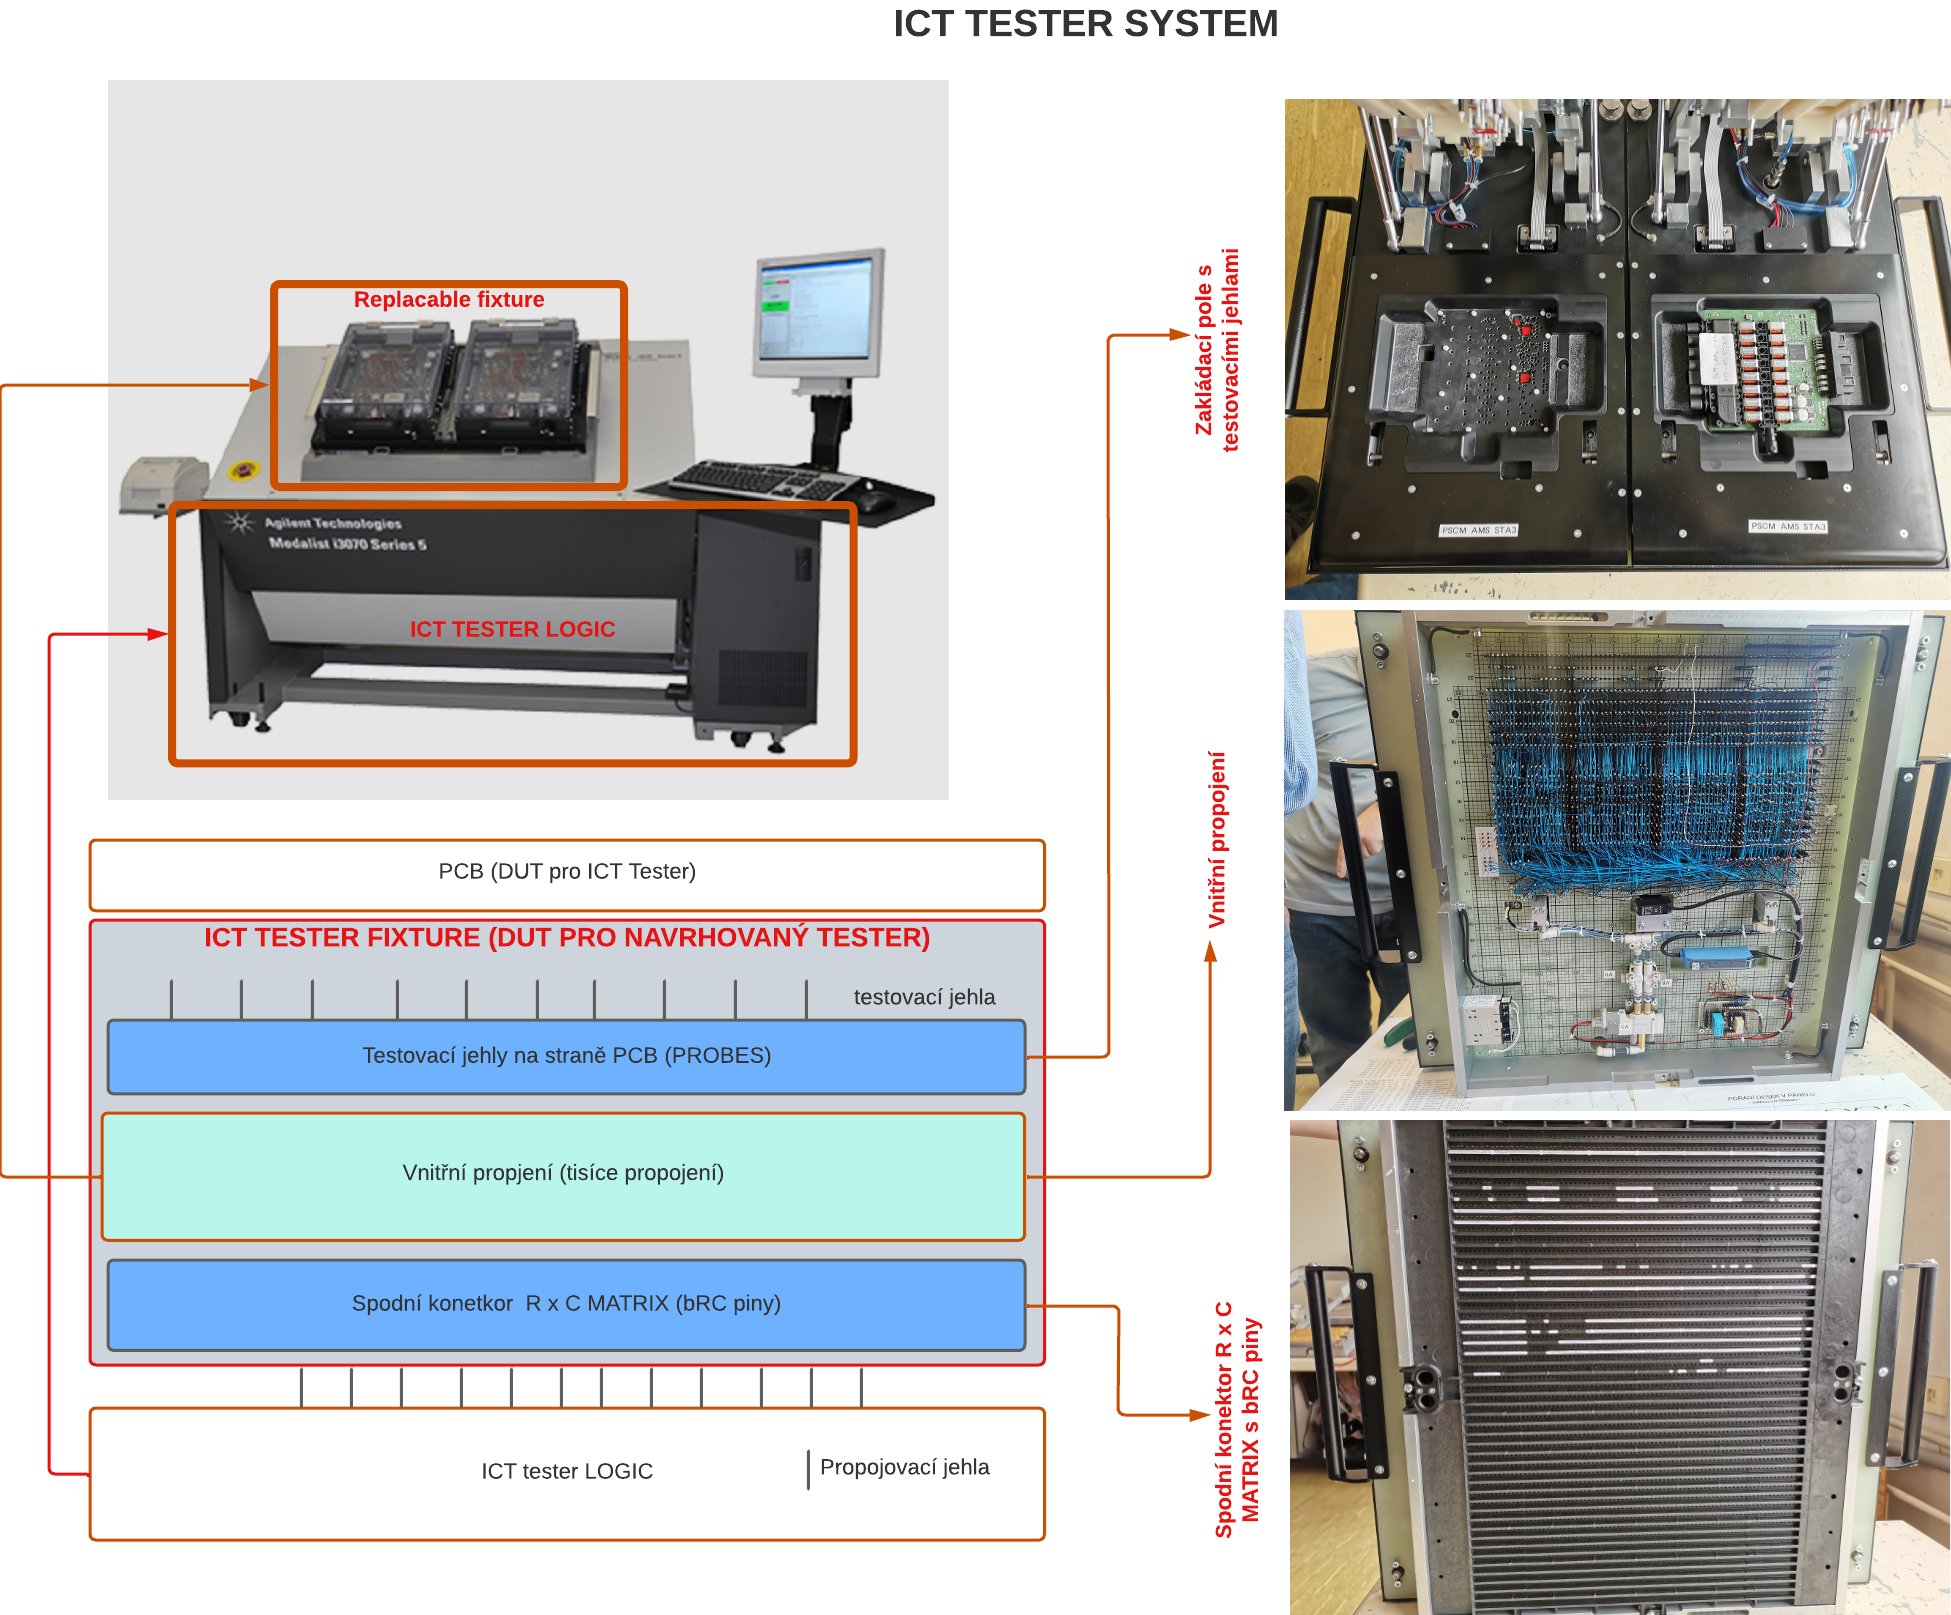
\includegraphics[width=0.9\textwidth]{obrazky/ICT_tester.png}
\caption{Části ICT testeru (obrázek testeru vlevo nahoře převzat z \cite{ICT_picture})}
\label{fig:ICT_tester}
\end{figure}
\clearpage

\section{Koncepce navrhovaného testeru}
Zatímco pro ICT tester bylo úkolem otestovat vložené PCB. Úkolem zařízení, navrhovaným v diplomové práci, je otestovat správnost propojení
fixture části ICT testeru. Pro tento účel je navržena následující koncepce.
\begin{figure}[ht!]
        \centering
        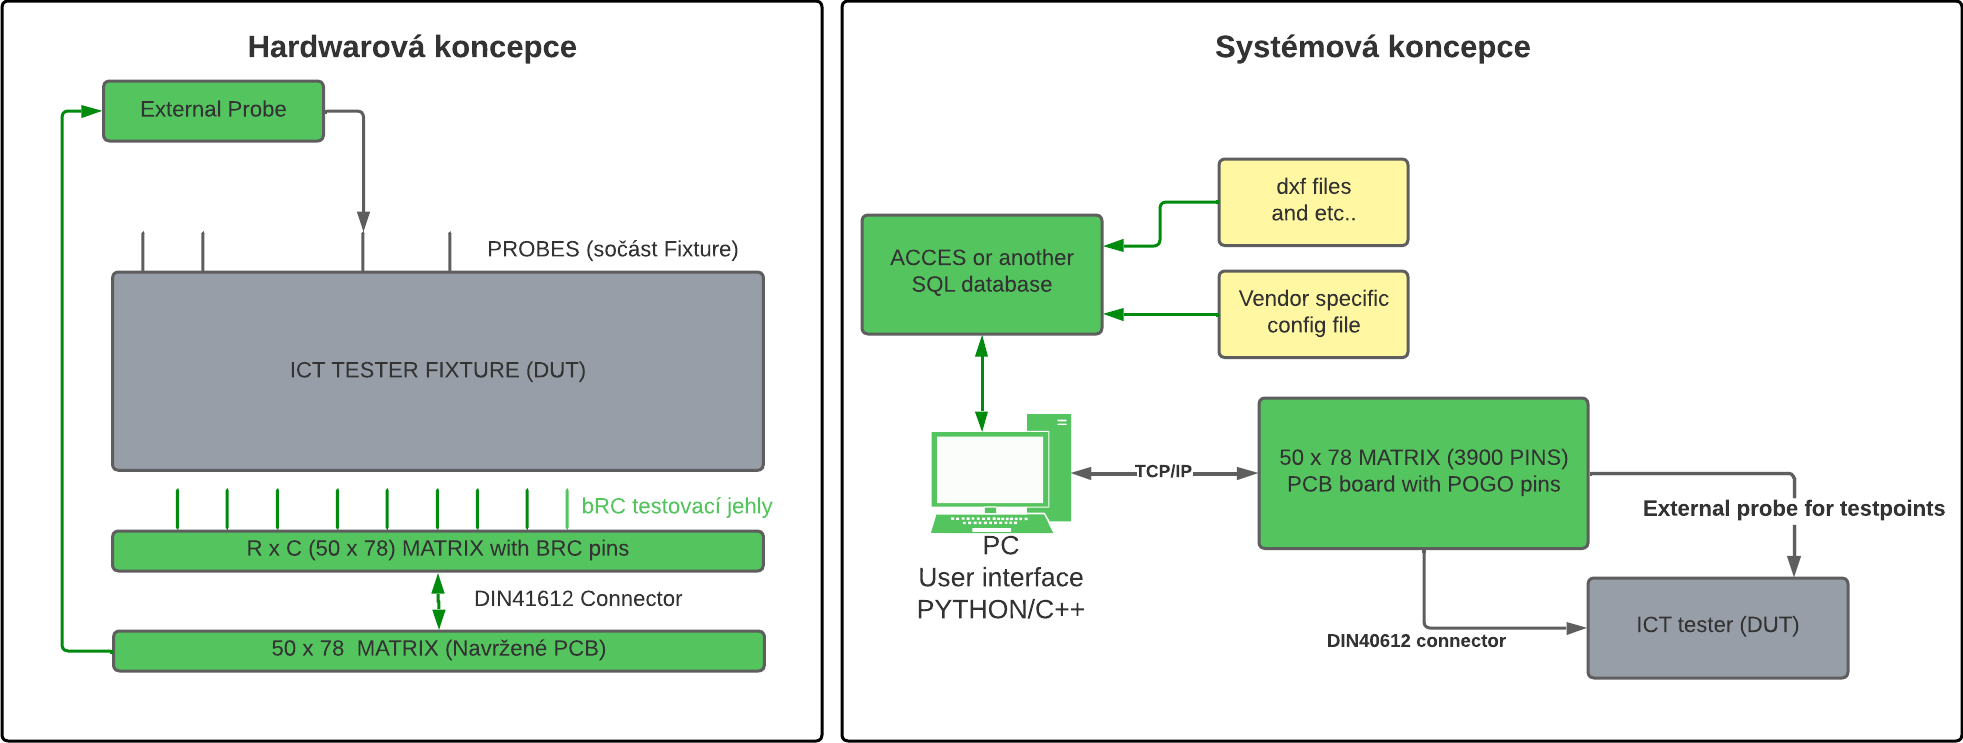
\includegraphics[width = 1\textwidth]{obrazky/system_connection_and_fixture.png}
        \caption{Koncepce funkčnosti navrhovaného testeru}
        \label{fig:Koncepce funkce}
    \end{figure}

    Na obrázku \ref{fig:Koncepce funkce} jsou zeleně znázorněny části, která jsou součástí diplomové práce.
    Ostatní barvy značí části, které již existují a nebudou navrhovány.
    \subsection{Systémová koncepce}
    Na obrázku \ref{fig:Koncepce funkce} v pravé části je znázorněná systémová koncepce testeru.
    Pro otestování vnitřního propojení fixture je nutné propojit všechny bRC piny s logikou navrhovaného testeru.
    Většina komerčních ICT testerů omezuje počet sloupců v bRC MATRIX na 78 a liší se tak pouze počtem řad.
    Z tohoto důvodu je tester navržen tak, aby bylo možné libovolně  měnit počet řad o 78 pinech\cite{ICT_guidline}.\\
    
    \begin{figure}[ht!]
        \centering
        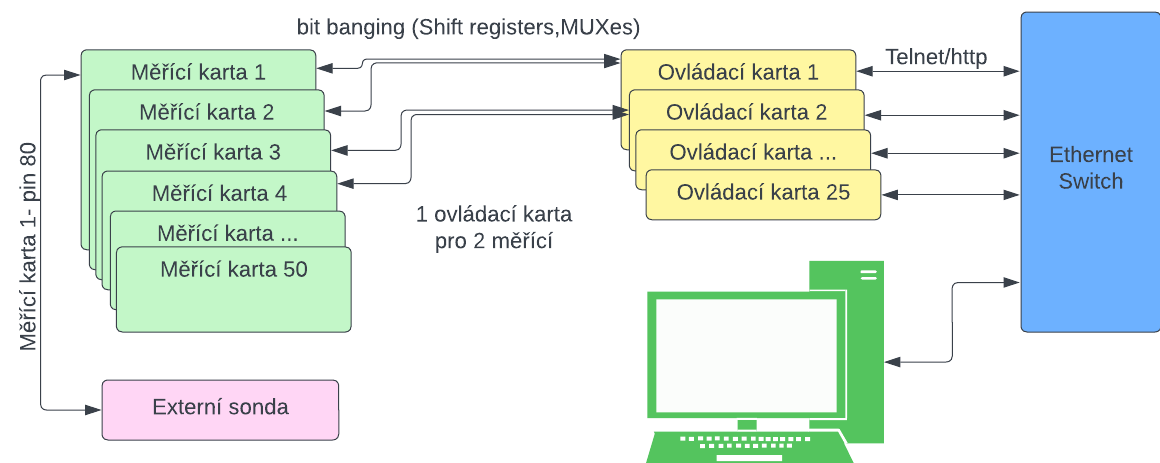
\includegraphics[width = 1\textwidth]{obrazky/telnet_http_pc.png}
        \caption{Systémová koncepce}
        \label{fig:Systémová koncepce}
    \end{figure}

    Navržené zařízení se skládá z měřících karet, ovládacích karet a řídícího počítače
    \mbox{(Obr. \ref{fig:Systémová koncepce})}.
    Úkolem měřící karty je měřit hodnoty odporu mezi jednotlivými bRC piny
    a odesílat data do ovládací karty. Měřící karty jsou kompatibilní s 5V a 3V3 logikou.\\

    \begin{figure}[ht!] 
        \centering
        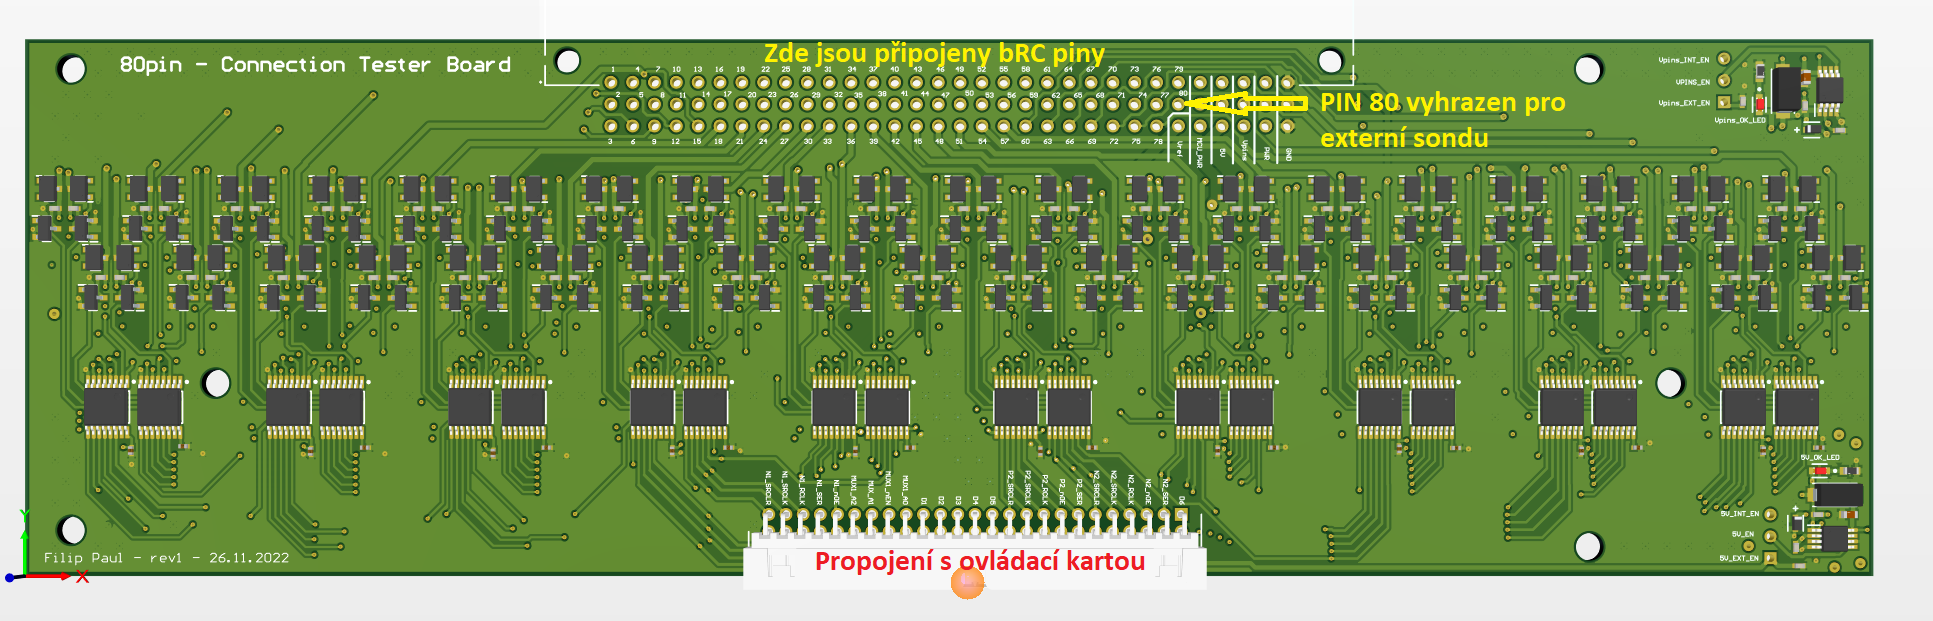
\includegraphics[width = 0.95\textwidth]{obrazky/karta_3D_NP.png}
        \caption{Měřící karta}
        \label{fig:Měřící karta}
    \end{figure}


    \begin{figure}[ht!]
        \centering
        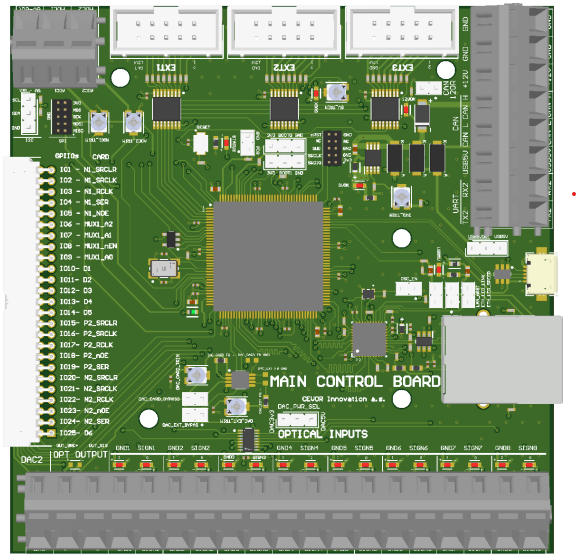
\includegraphics[width = 1\textwidth]{obrazky/3D_ovl_karta.png}
        \caption{Ovládací karta - 3D model (Není vyrobena jedná se o předběžný návrh)}
        \label{fig:Ovládací karta - 3D model}
    \end{figure}

    Jednotlivé ovládací karty mají možnost připojení k ethernetové síti pomocí
    100BASE-T PHY a jsou schopny ovládat až 2 měřící karty zároveň.
    Ovládací karty komunikují pouze s řídící PC aplikací (nikoliv mezi sebou).
    Řídící PC aplikace řídí všechny testy. Ovládací karty mají v sobě implementován Telnet a http server,
    přičemž se pro hlavní komunikaci používá právě Telnet server.
    Takto lze využít jakékoliv zařízení s přístupem do sítě pro řízení testeru.\\
    
    Řídící aplikace využívá ke své činnosti celou řadu vstupních souborů. Jedná se o soubory, které definují zapojení fixture, CAD, CAM a další data\cite{CAD_wiki}.
    Protože vstupní soubory nemají jednotný formát pro každého výrobce, aplikace nejprve data převede do SQL databáze (ACCESS). S takto zpracovanými daty již lze
    provádět jednotné operace. Aplikace porovnává naměřená data z jednotlivých karet ze vstupními soubory a následně generuje výsledek testu propojení
    v co nejsrozumitelnější podobě.

    \subsection{Hardwarová koncepce}
    \subsubsection{Propojení bRC pinů mezi sebou}

    Propojení mezi měřícími kartami a maticí bRC pinů je zajištěno pomocí POGO pinů (strana fixture),
    bRC jehel (strana testeru) a pneumatického kontaktování.
    Na Obr. \ref{fig:Měřící karta} je znázorněn 3D model měřící karty. V horní části jsou připraveny 
    body pro připojení bRC jehel a napájení desky. Rozteč kontaktů je zvolena tak, aby bylo možno
    k měřící kartě připájet standardizovaný DIN41612 konektor (dále pouze DIN) a kartu tak snadno použít pro jiné aplikace.\\

    Ve spodní části se nachází 25x2 konektor, sloužící k propojení s ovládací kartou. Měřící karta je navržena tak, aby buď poskytovala
    napájení ovládací kartě a nebo byla ovládací kartou napájena (více v sekci o návrhu měřící karty).

    \subsubsection{Propojení mezi bRC a Probes}
    Pomocí karet je možné automaticky zjistit propojení mezi všemi bRC piny,
    nicméně přímé propojení mezi bRC a Probe piny je nutné otestovat zvlášť.
    Za tímto účelem je k testeru připojena externí sonda (Obr. \ref{fig:Systémová koncepce}).
    Sonda je připojena do bRC pinu \hbox{č. 80} na měřící
    kartě \hbox{č. 1.}\\

    Obsluha v závislosti na pokynech PC aplikace připojuje sondu k jednotlivým probes pinům.
    Takto lze pomocí jednotlivých karet zjistit propojení.
    Externí sonda je podobná jako sonda multimetru a slouží pouze k přivedení testovacího napětí na probe pin.
    Proces lze celý automatizovat v případě, že je k dispozici i maketa PCB,
    která bude obsahovat všechny probe piny přivedené na DIN konektor.
    V takovém případě lze připojit maketu PCB k kartě a proces automatizovat.

    \chapter{Návrh měřících karet}
    Tato kapitola se zabývá hardwarovým řešením měřících karet. Dále je zde popsána funkčnost základních bloků karet, výběr komponentů a návrh PCB.

    \section{Základní požadavky na měřící karty}
    Následující seznam popisuje základní požadavky na měřící karty, seznam je seřazen podle priorit.
    \begin{enumerate}
        \item Schopnost měřit odpor mezi jakýmikoliv dvěma bRC piny a to i v případě, že se každý z pinů nachází na jiné kartě.
        \item Komunikace s ovládací kartou.
        \item Škálovatelnost.
        \item Modularitou se rozumí, co největší nezávislost jednotlivých funkčních bloků na sobě.
        \item Dostupnost komponentů. 
        \item Cena komponentů. 
    \end{enumerate}

    \section{Funkční bloky}
    Na následujícím obrázku je znázorněn blokový diagram měřících karet.
    \begin{figure}[ht!]
            \centering
            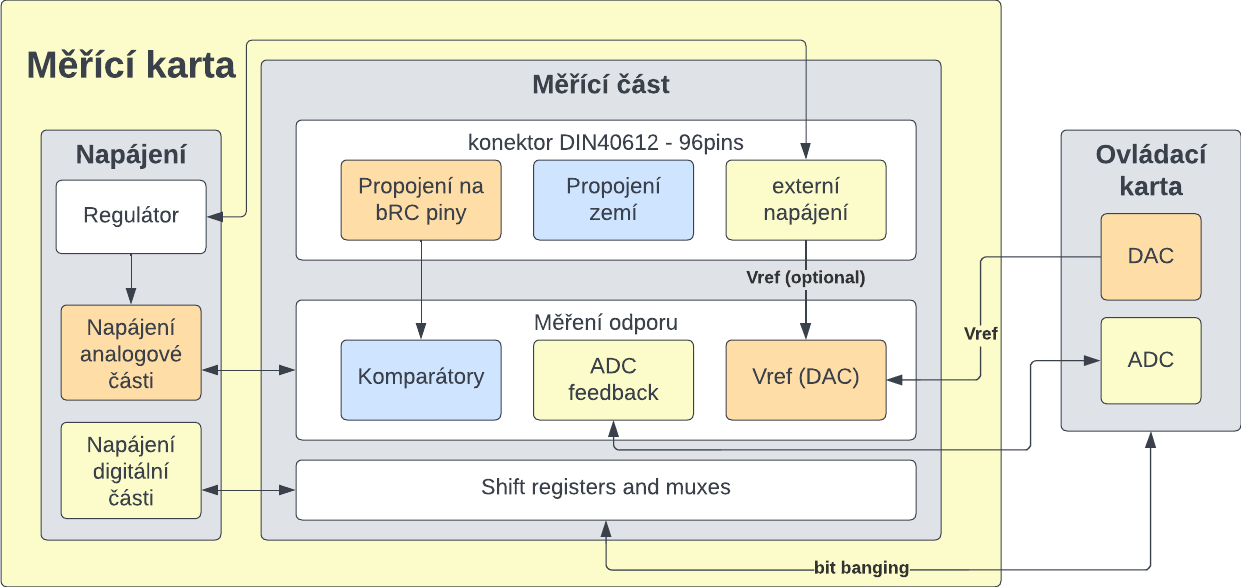
\includegraphics[width = 1\textwidth]{obrazky/karta_system_diagram.png}
            \caption{Blokový diagram měřících karet}
            \label{fig:Blokový diagram měřících karet}
    \end{figure}

        Karta se skládá ze 2 hlavních bloků (Měřící části a napájení). V následujících kapitolách jsou tyto bloky
        podrobně popsány.
        \clearpage

        \subsection{Měřící část}
        \subsubsection{Teoretický návrh}
        Měřící část je zodpovědná za měření odporu mezi dvěma bRC piny.
        Obr. \ref{fig:Napěťový dělič pro 2 a 4 propojené bRC piny} v levé části zobrazuje
        jednoduchý ideální napěťový dělič.
        Dělič je zapojen tak, že jeden z testovaných pinů bRC1 generuje napětí $V_{in}$
        a na druhém pinu bRC2 se měří napětí $V_{out}$.
        Měřeným odporem je odpor Rpath, který lze dopočítat následovně:\\
        
        \begin{equation}\label{eq:odpor delic}
            R_{path} = \frac{(V_{in} - V_{out}) \cdot R_x}{V_{out}}
        \end{equation}
        
    \begin{figure}[ht!]
            \centering
            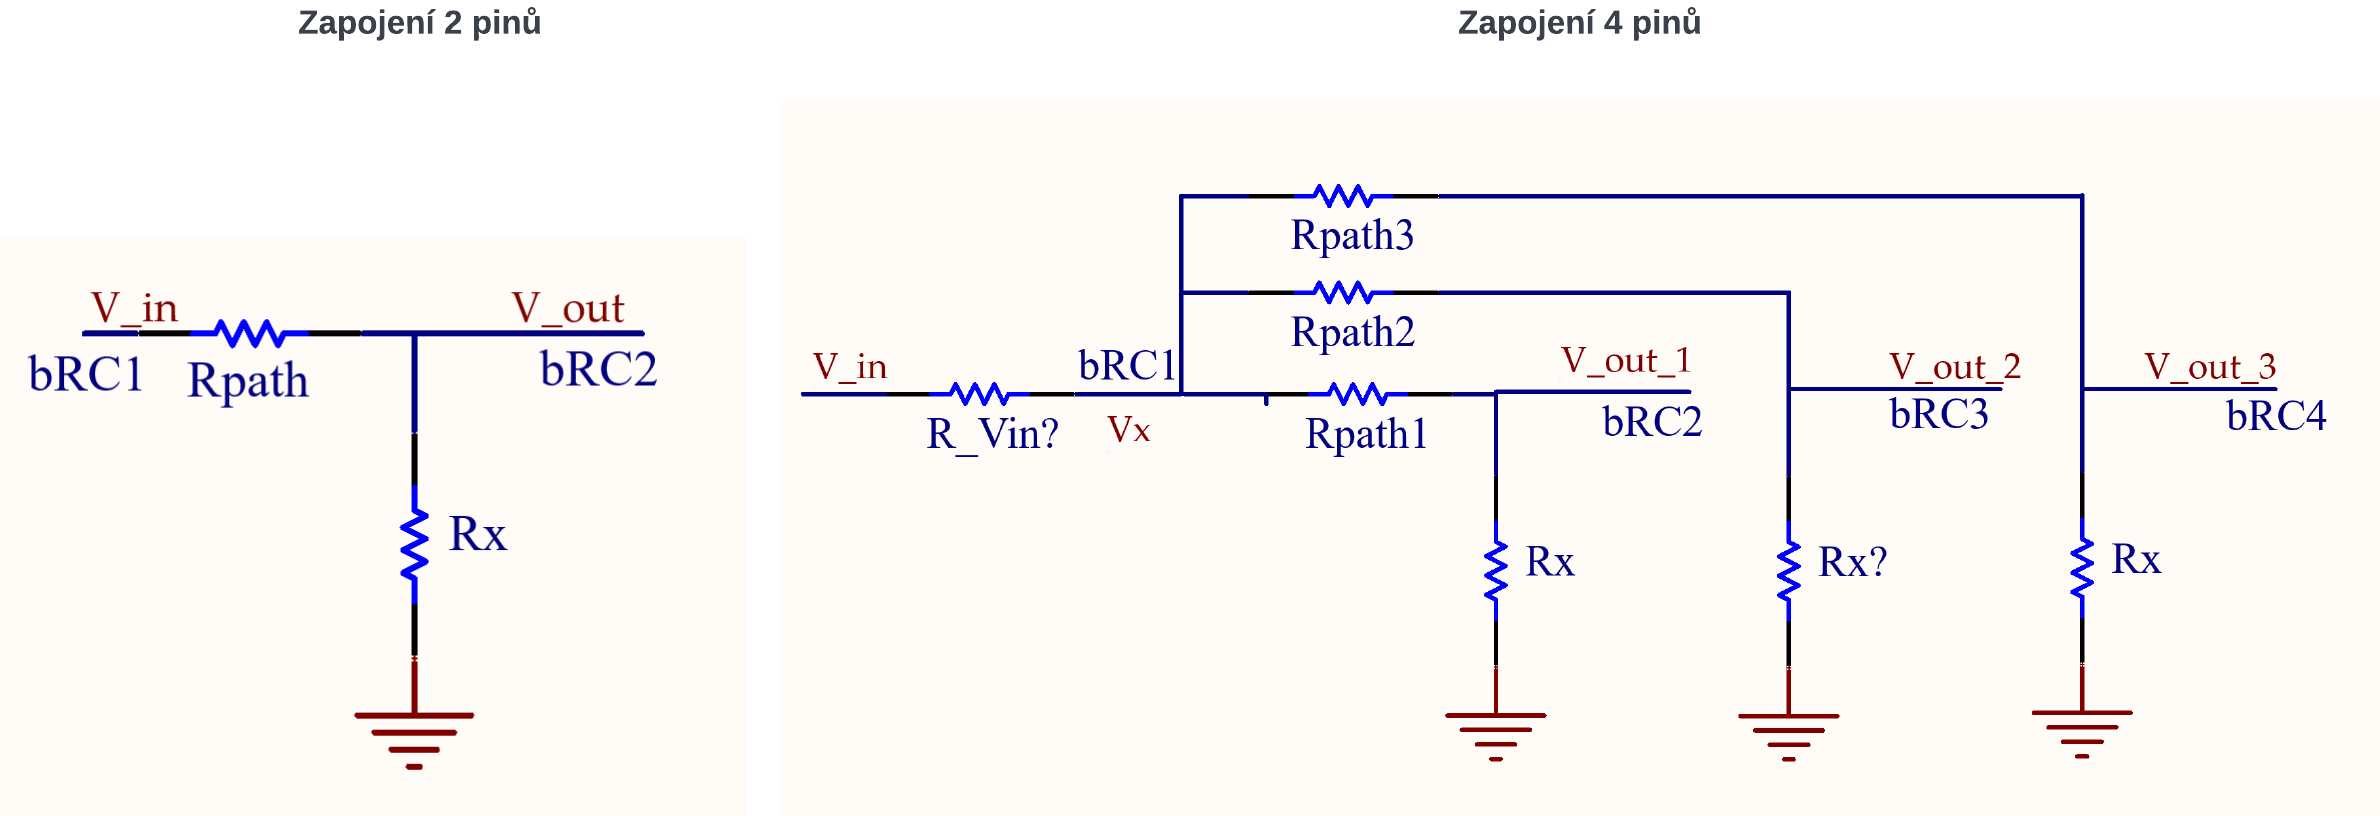
\includegraphics[width = 1\textwidth]{obrazky/2_and_4_pins_connection.png}
            \caption{Napěťový dělič pro 2 a 4 propojené bRC piny}
            \label{fig:Napěťový dělič pro 2 a 4 propojené bRC piny}
    \end{figure}

    Fixture může mít vnitřní zapojení takové, že se vzájemně propojí více než dva bRC piny. V takovém případě by pro např. 4 propojené bRC piny situace
    vypadala jako na obrázku v pravé části, kde odpory Rpath1 až Rpath3 značí odpory jednotlivých cest mezi piny. V\_out\_1 až V\_out\_3 značí napětí na
    výstupech děličů. V případě ideálního zdroje napětí (na obrázku značeno jako Vx) by obvod stále fungoval a platila by
    rovnice \ref{eq:odpor delic} . Do obvodu by však tekl 3-násobný proud.\\
    
    V případě reálného zdroje napětí se uplatňuje jeho vnitřní odpor $R_{Vin}$ a především úbytek napětí vzniklý na tomto odporu.
    Vzhledem k tomu, že úbytek napětí, na vnitřním odporu zdroje, je úměrný protékajícímu proudu a zároveň proud je úměrný počtu propojených pinů, kterých může být
    v případě zemních smyček fixture mnoho. Vzniká potřeba možnosti odpojení jednotlivých bRC pinů. Odpojení bRC pinu je zajištěno pomocí N-channel mosfetu
    \hbox{(obr. \ref{fig:Napěťový dělič pro s možností high Z vstupem}).}
    Toto zapojení v případě nulového napětí na vstupu mosfetu vytvoří vysokou impedanci na vstupu
    pinu, kterým pak protéká pouze zanedbatelný proud. V případě, že je na vstupu napětí vyšší než prahové napětí mosfetu, výpočet odporu se pro ideální zdroj napětí
    změní následovně.
    \begin{equation}
        R_{path} = \frac{(V_{in} - V_{out}) \cdot (R_x + N_{RDSon}) }{V_{out}},
    \end{equation}
     kde $N_{RDSon}$ je odpor otevřeného mosfetu.\\

\clearpage
    \begin{figure}[ht!]
        \centering
        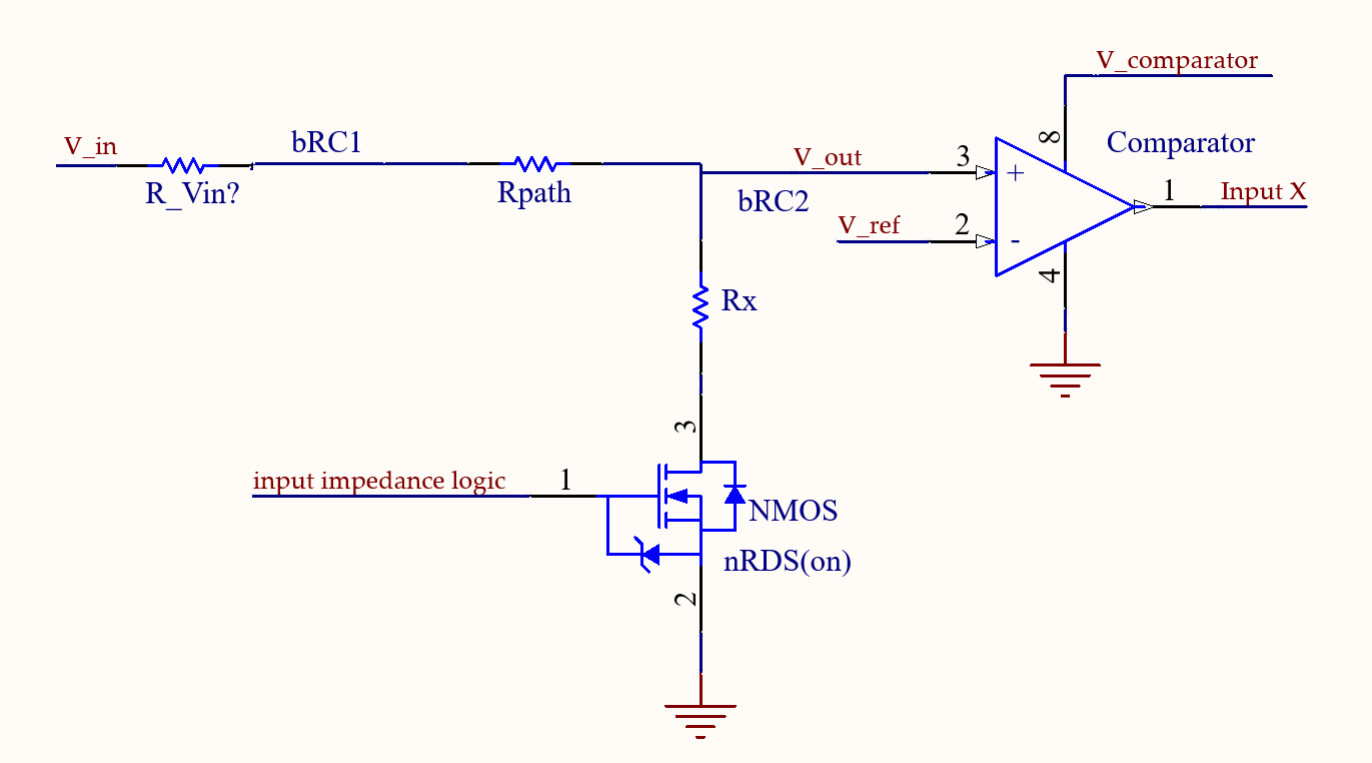
\includegraphics[width = 1\textwidth]{obrazky/nMos_Connection.png}
        \caption{Napěťový dělič pro s možností high Z vstupem}
        \label{fig:Napěťový dělič pro s možností high Z vstupem}
\end{figure}

    Další nevýhodou zapojení na obr.\ref{fig:Napěťový dělič pro 2 a 4 propojené bRC piny}
    je nutnost měření analogového napětí na každém pinu, což by vedlo k
    složitosti zapojení a vysokým nákladům na výrobu. Naprostá většina bRC pinů je propojená jako zkrat a zajímá nás především,
    zda hodnota odporu propojení nepřekračuje nějakou mez.
    Toho lze využít připojením komparátoru na výstup děliče (Obr.\ref{fig:Napěťový dělič pro s možností high Z vstupem}).
    Komparátor porovnává výstupní napětí $V_{out}$ s hodnotou referenčního napětí $V_{ref}$.\\

    Referenční napětí je nastavováno pomocí 12-bit D/A převodníku ovládací desky. V případě nastavení referenčního napětí
    pro určitou mezní hodnotu Rpath,
    lze kontrolovat pouze logickou hodnotu výstupu $V_{comparator}$
    (na obr.\ref{fig:Napěťový dělič pro s možností high Z vstupem} jako InputX).
    V případě, že bude nutné změřit reálný odpor cesty, je možné měnit napětí $V_{ref}$ a sledovat při jaké hodnotě se 
    komparátor překlopí.\\

    Další otázkou je, jak generovat napětí $V_{in}$ na vstupu děliče.
    Protože každý bRC pin musí být zároveň vstupní i výstupní, musí být konfigurovatelný do vysoké impedance (HIGH Z).
    Zároveň pokud bude každý pin schopen dodat do obvodu dostatečné množství proudu,
    bude možné měřit odpor několika cest současně.
    Řešením je obvod na obr.\ref{fig:Zapojení měřící části s p-channel MOSFET}.\\

    V tomto zapojení přibyl P-channel mosfet,
    který umožňuje spínat (ovládat) výstupní napětí V\_in.
    Nicméně vzniká zde obdobný problém jako u zapojení na obr.\ref{fig:Napěťový dělič pro 2 a 4 propojené bRC piny} a to,
    že s rostoucím proudem roste úbytek napětí na vnitřním odporu zdroje charakterizovaným
    odporem $R_{Vin}$. Z tohoto důvodu je úbytek monitorován 12 bitovým A/D převodníkem (na ovládací kartě).
    Výsledek měření odporu je pak vztažen k hodnotě změřené pomocí A/D převodníku.
    Odpor zdroje se pak bude rovnat $R_{DSon}$ P-channel mosfetu.
    Nastává tak problém určit vliv odporu $R_{DSon}$ na výslednou hodnotu změřeného odporu Rpath\cite{HOROWITZ,MARTINT}.
    \clearpage

    Protože každý pin může být zároveň výstupní i vstupní, kde vstupní funkci plní lokální komparátor.
    Lze pro přesné měření změřit přímo výstupní napětí V\_out\_local pomocí lokálního komparátoru a vliv $R_{DSon}$ úplně eliminovat.
    Nicméně tato metoda je časově náročnější a je více diskutována v kapitole o algoritmizaci.\\
        
    %\noindent
    %$R_{path} = \frac{V_{ADC} \cdot (R_{NMOS}+ R_{X}) }{V_{out}} - R_{NMOS} - R_{X} - R_{PMOS}$,\\\\
    %kde $R_{NMOS}$ a $R_{PMOS}$ jsou hodnoty RDSon otevřených P a N mosfetů.\\
\begin{figure}[ht!]
        \centering
        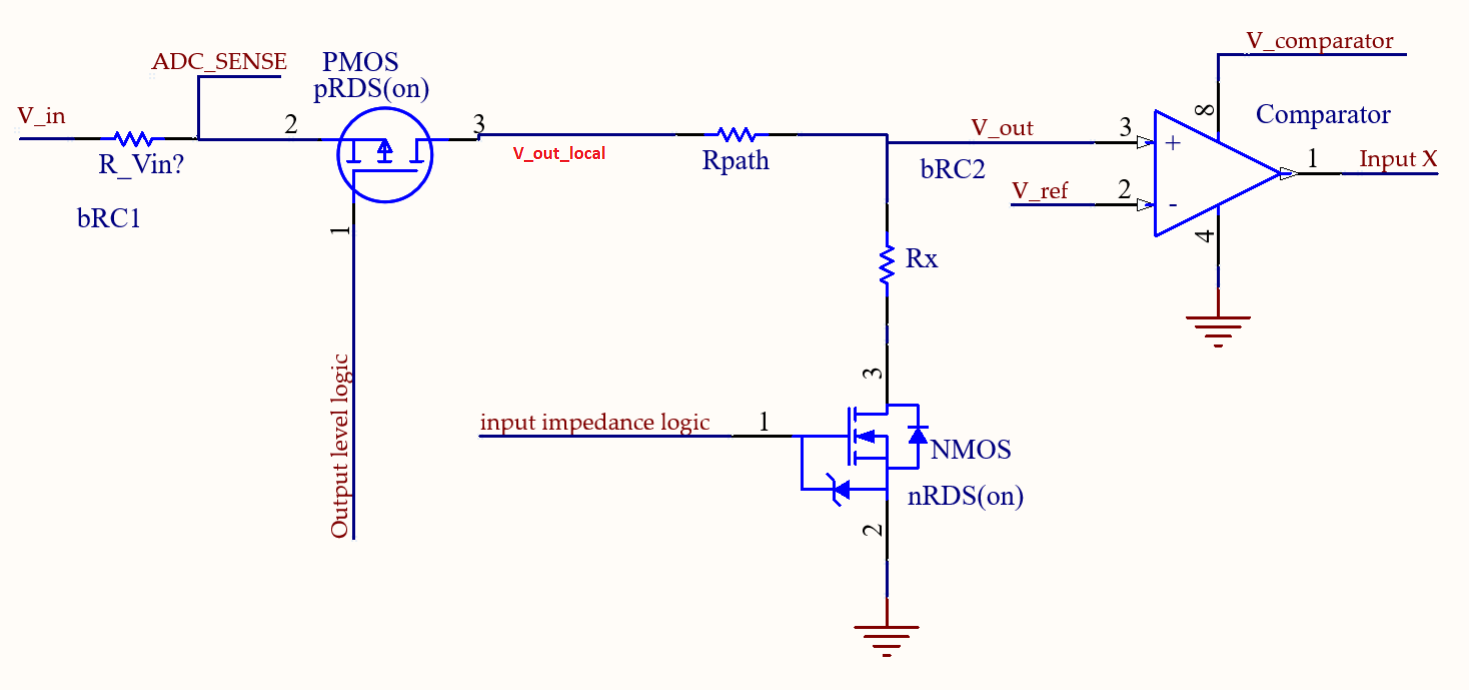
\includegraphics[width = 1\textwidth]{obrazky/final_connection.png}
        \caption{Zapojení měřící části s p-channel MOSFET}
        \label{fig:Zapojení měřící části s p-channel MOSFET}
\end{figure}

    Ve schématu na obr.\ref{fig:Zapojení měřící části s p-channel MOSFET}
    si lze všimnout řídících napětí (Output level logic, input impedance logic a input X).
    Output level logic řídí, zda generuje rBC pin napětí.
    Input impedance logic umožňuje nastavit HIGH Z na vstupním obvodu. Input X je výstup komparátoru. Vzniká
    tak potřeba pro každý bRC pin mít 2 logické výstupy a jeden vstup. Každá deska musí mít minimálně 78 bRC pinů,
    což znamená minimálně 156 logických výstupů a 78 logických vstupů.\\

    Pro tento účel je použito pro nastavení 78x Output level logic 2x5x8-bit shift registrů zapojených do série.
    Obdobně je pro nastavení 78x input impedance logic je použito 2x5x8-bit shift registrů zapojených do série.
    a pro 78 logických výstupů je použito 2x5x8-bit multiplexerů se společnou adresací.
    Společnou adresací se rozumí, že adresy 2x5 multiplexerů jsou řízeny 2x3 adresními piny.
    Vzhledem k použití 8-bit komponentů je výsledný počet bRC pinů na desce zaokrouhlen na 80 místo 78,
    přičemž 2 poslední vstupy/výstupy jsou na testeru ignorovány
    (v případě měřící desky č.1 je pin č. 80 použit pro externí sondu). 
    Hierarchické schéma měřící karty lze nalézt v příloze.\\

    Měřící karty fungují, vzhledem k potřebám testování, ve dvou režimech (PASS/FAIL a měření reálného odporu).
    PASS/FAIL režim je určen pro rychlé hromadné otestování všech pinů,
    kde hlavním kritériem je, zda propojení mezi piny odpovídají nějaké mezní hodnotě odporu nebo ne.
    Výsledkem je pak pouze mapa propojení bez hodnot reálného odporu.
    Režim měření reálného odporu pak umožňuje změřit co nejpřesnější hodnotu odporu všech propojení.
\clearpage
\subsubsection{Výběr součástek a volba jejich hodnoty}
V předchozí sekci byla diskutována funkčnost zapojení.
Nicméně nebylo doposud zmíněno, jaké kvantitativní hodnoty součástek jsou vhodné pro realizaci.
V této sekci jsou popsány konkrétní reálné součástky, které byly použity včetně zdůvodnění jejich výběru.\\

\subsubsection{Volba velikosti odporu děliče Rout}
\textbf{Odvození podmínek pro výběr odporu děliče:}\\
V celé následující sekci je zanedbán vliv komparátoru na měřící obvod.
V první řadě je nutné definovat jaká je vyžadovaná přesnost, rozsah a rychlost měření.
Vzhledem k charakteru propojení ve fixture by měl být tester schopen změřit odpor v rozsahu od 1\,$\Omega$ do 1\,k$\Omega$.
Vyžadované rozlišení je 1$\Omega$ především pro odpory do 100\,$\Omega$.
Co se týče rychlosti měření, tak pro automatické měření mezi dvěma bRC piny nejsou kladeny žádné požadavky,
protože je proces plně automatizován.\\
Při měření odporu mezi bRC a Probe piny, obsluha postupně testuje všechny piny všech karet zvlášť externí sondou.
V tomto případě by prodleva mezi přiložením sondy a vyhodnocením signálu neměla být pro
člověka rozpoznatelná (signalizace pískáním obdobně jako continuity test multimetru).
Z tohoto důvodu je nutné pro jeden pin změřit propojení mezi všemi ostatními piny
do cca 40\,ms (včetně komunikací s PC cca. 30\,ms).
Nicméně stačí vyhodnocovat PASS/FAIL pro odpor cesty a ne přímo jeho hodnotu.
Následující tabulka je shrnutím tohoto odstavce.\\


\begin{table}[ht!]
    \resizebox{\textwidth}{!}{%
    \begin{tabular}{|lccccc|}
    \hline
    \multicolumn{6}{|c|}{\textbf{Požadované charekteristiky měřícího obvodu}}                                                                                                                                                                                                                                                                                  \\ \hline
    \multicolumn{1}{|l|}{\textbf{TEST MODE}}                & \multicolumn{1}{c|}{\textbf{Počet pinů}} & \multicolumn{1}{c|}{\textbf{Rozsah $[\Omega]$}}  & \multicolumn{1}{c|}{\textbf{Přesnost $[\pm \Omega]$}} & \multicolumn{1}{c|}{\textbf{čas $[\mu s/pin]$}} & \textbf{Celkový čas $[ms]$} \\ \hline
    \multicolumn{1}{|l|}{\textbf{PASS/FAIL}}                & \multicolumn{1}{c|}{4000}                & \multicolumn{1}{c|}{1-1000}                      & \multicolumn{1}{c|}{2}                                & \multicolumn{1}{c|}{2,5}                        & 10                          \\ \hline
    \multicolumn{1}{|l|}{\textbf{Měření   "pravé"\ hodnoty}} & \multicolumn{1}{c|}{4000}                & \multicolumn{1}{c|}{1-1000}                      & \multicolumn{1}{c|}{1}                                & \multicolumn{1}{c|}{Nedefinován}                & Nedefinován                 \\ \hline
    \end{tabular}%
    }
    \caption{Požadované měřící charakteristiky}
    \label{tab:Požadované měřící charakteristiky}
\end{table}

Všechna následující odvození vycházejí z následující výchozí rovnice pro výstup napěťového děliče pro 2 propojené bRC piny:

\begin{equation}
V_{out} = \frac{ V_{in}\cdot R_{out} }  {R_{out} + R_{path} + R^P_{DSon}},
\end{equation}

kde ${R_{out}} = R_X + R^N_{DSon}$ a $R^P_{DSon}$ je ekvivalent $R_{Vin}$ a odpovídá odporu P-channel mosfetu. \\

Z tabulky vyplývá několik podmínek pro volbu rezistoru ${R_{out}}$. První podmínka se vztahuje k přesnosti měření. Přesnost měření ovlivňují převážně 2 faktory.
Prvním faktorem je chyba vzniklá diskretizací referenčního napětí komparátoru,
které je generováno 12bit D/A převodníkem. Protože rovnice pro výstupní napětí děliče je nelineární
bude nelineární i chyba vzniklá kvantováním. Podmínku pro splnění přesnosti, v případě, že se projeví pouze kvantizační chyba, lze vyjádřit následovně:

\begin{equation}
\left| \frac{\partial V_{out} }{\partial R_{path}}\cdot \Delta R_{path} \right| > \frac{V_{ref}}{2^{12}},
\end{equation}

kde $\left| \frac{\partial V_{out} }{\partial R_{path}}\cdot \Delta R_{path} \right|$
značí změnu napětí Vout způsobenou změnou $R_{path}$ o
požadovanou přesnost v $\Omega$ a $R_{path}$ je z rozsahu 0 - 1k\,$\Omega$.
Tento vztah se také dá reprezentovat jako citlivost měření na změnu $R_{path}$.\\

Druhým faktorem, ovlivňujícím přesnost je chyba, kterou do měření přidává odpor $R^P_{DSon}$ P-channel mosfetu při paralelním měření několika bRC pinů.
Tato chyba roste s zvyšujícím se proudem a projeví se tak především při PASS/FAIL režimu.
Vzhledem k náhodnému vnitřnímu propojení fixture není možno dopředu odhadnout, kolik bRC pinů bude připojeno a tak ani výsledný proud odporem $R^P_{DSon}$.
Uvažujme, že chceme změřit "nejhorší scénář"\ (všechny piny jsou mezi sebou propojeny tvrdým zkratem).
Následně poteče obvodem proud přibližně:

\begin{equation}
I = \frac{V_{in}}{R_{out}/N_{pins} + R^P_{DSon}}
\end{equation}

 Proud je tak nepřímo úměrný velikosti hledaného odporu Rout a počtu paralelně měřených pinů.
 Pokud bychom chtěli změřit všechny piny na kartě současně ($N_{pins}$ = 80).
 Musí každý pin být schopen dodat do obvodu proud $I = 80 \cdot V_{in}/R_{out}$.
 Vzhledem k nenulovému odporu $R^P_{DSon}$, který lze připodobnit
 vnitřnímu odporu zdroje napětí vzniká následující podmínka pro nejhorší možný případ:

 \begin{equation}
    I \cdot {R^P_{DSon}}  < \left| \frac{\partial V_{out} }{\partial R_{path}}\cdot \Delta R_{path} \right|\
\end{equation}

\begin{equation}
   \frac{V_{in} \cdot R^P_{DSon}}{R_{out}/N_{pins} + R^P_{DSon}} < \left| \frac{\partial V_{out} }{\partial R_{path}}\cdot \Delta R_{path} \right|
\end{equation}
Podmínka vyjadřuje, že chyba vzniklá úbytkem napětí na $R^P_{DSon}$ za předpokladu Npins propojených pinů,
by na výstupu děliče Vout neměla být větší než nejnižší napětí, které vznikne změnou odporu cesty o požadovanou přesnost v\,$\Omega$. \\

Při uvážení nejhoršího scénáře, že se sečte chyba dána kvantováním a chyba dána odporu $R^P_{DSon}$, lze vyjádřit podmínku pro hledaný odpor
$R_{out}$ následovně:

\begin{equation}\label{eq:citilivost}
\frac{V_{ref}}{2^{12}} + \frac{V_{in} \cdot R^P_{DSon}}{R_{out}/N_{pins} + R^P_{DSon}} < \left| \frac{\partial V_{out} }{\partial R_{path}}\cdot \Delta R_{path} \right|
\end{equation}
\\
\textbf{Řešení podmínek výběru hodnoty odporu děliče:}\\
    Rovnici \ref{eq:citilivost} lze považovat za citlivost obvodu na změnu odporu $R^P_{DSon}$.
    Řešením by měla být být oblast hodnot, ve které odpor $R_{out}$ splňuje podmínky pro přesnost.
    Kvůli názornosti byla zvolena grafická metoda řešení.
    Následující obrázek \ref{fig:3D zobrazení rovnice pro výstupní napětí děliče}
    ukazuje výstupní napětí ideálního děliče v závislosti na odporu $R_{out}$ a $R_{path}$.
    V levé části je zobrazena celá zkoumaná oblast a v pravé části je stejný graf zobrazen z "bočního"\ pohledu.
    V takovém zobrazení je patrné, jaká je změna výstupního napětí $V_{out}$ při změně odporu $R_{path}$.
    Pokud zobrazíme 2 sousední hodnoty výstupního napětí tak, aby náležely stejnému odporu $R_{out}$ (leží vertikálně nad sebou).
    Rozdílem těchto 2 hodnot získáme citlivost
    $\left| \frac{\partial V_{out} }{\partial R_{path}}\cdot \Delta R_{path} \right|$.
    Na obrázku je z důvodu lepšího zobrazení zvolena velká změna odporu $\Delta R_{path}$
    (v tomto případě 20\,$\Omega$).
    Pro správný návrh je pak nutné zvolit stejnou změnu odporu $\Delta R_{path}$ jako má požadovaná přesnost\cite{Sensitivity_embedded,Sensitivity_2}.\\

\begin{figure}[ht!]
    \centering
    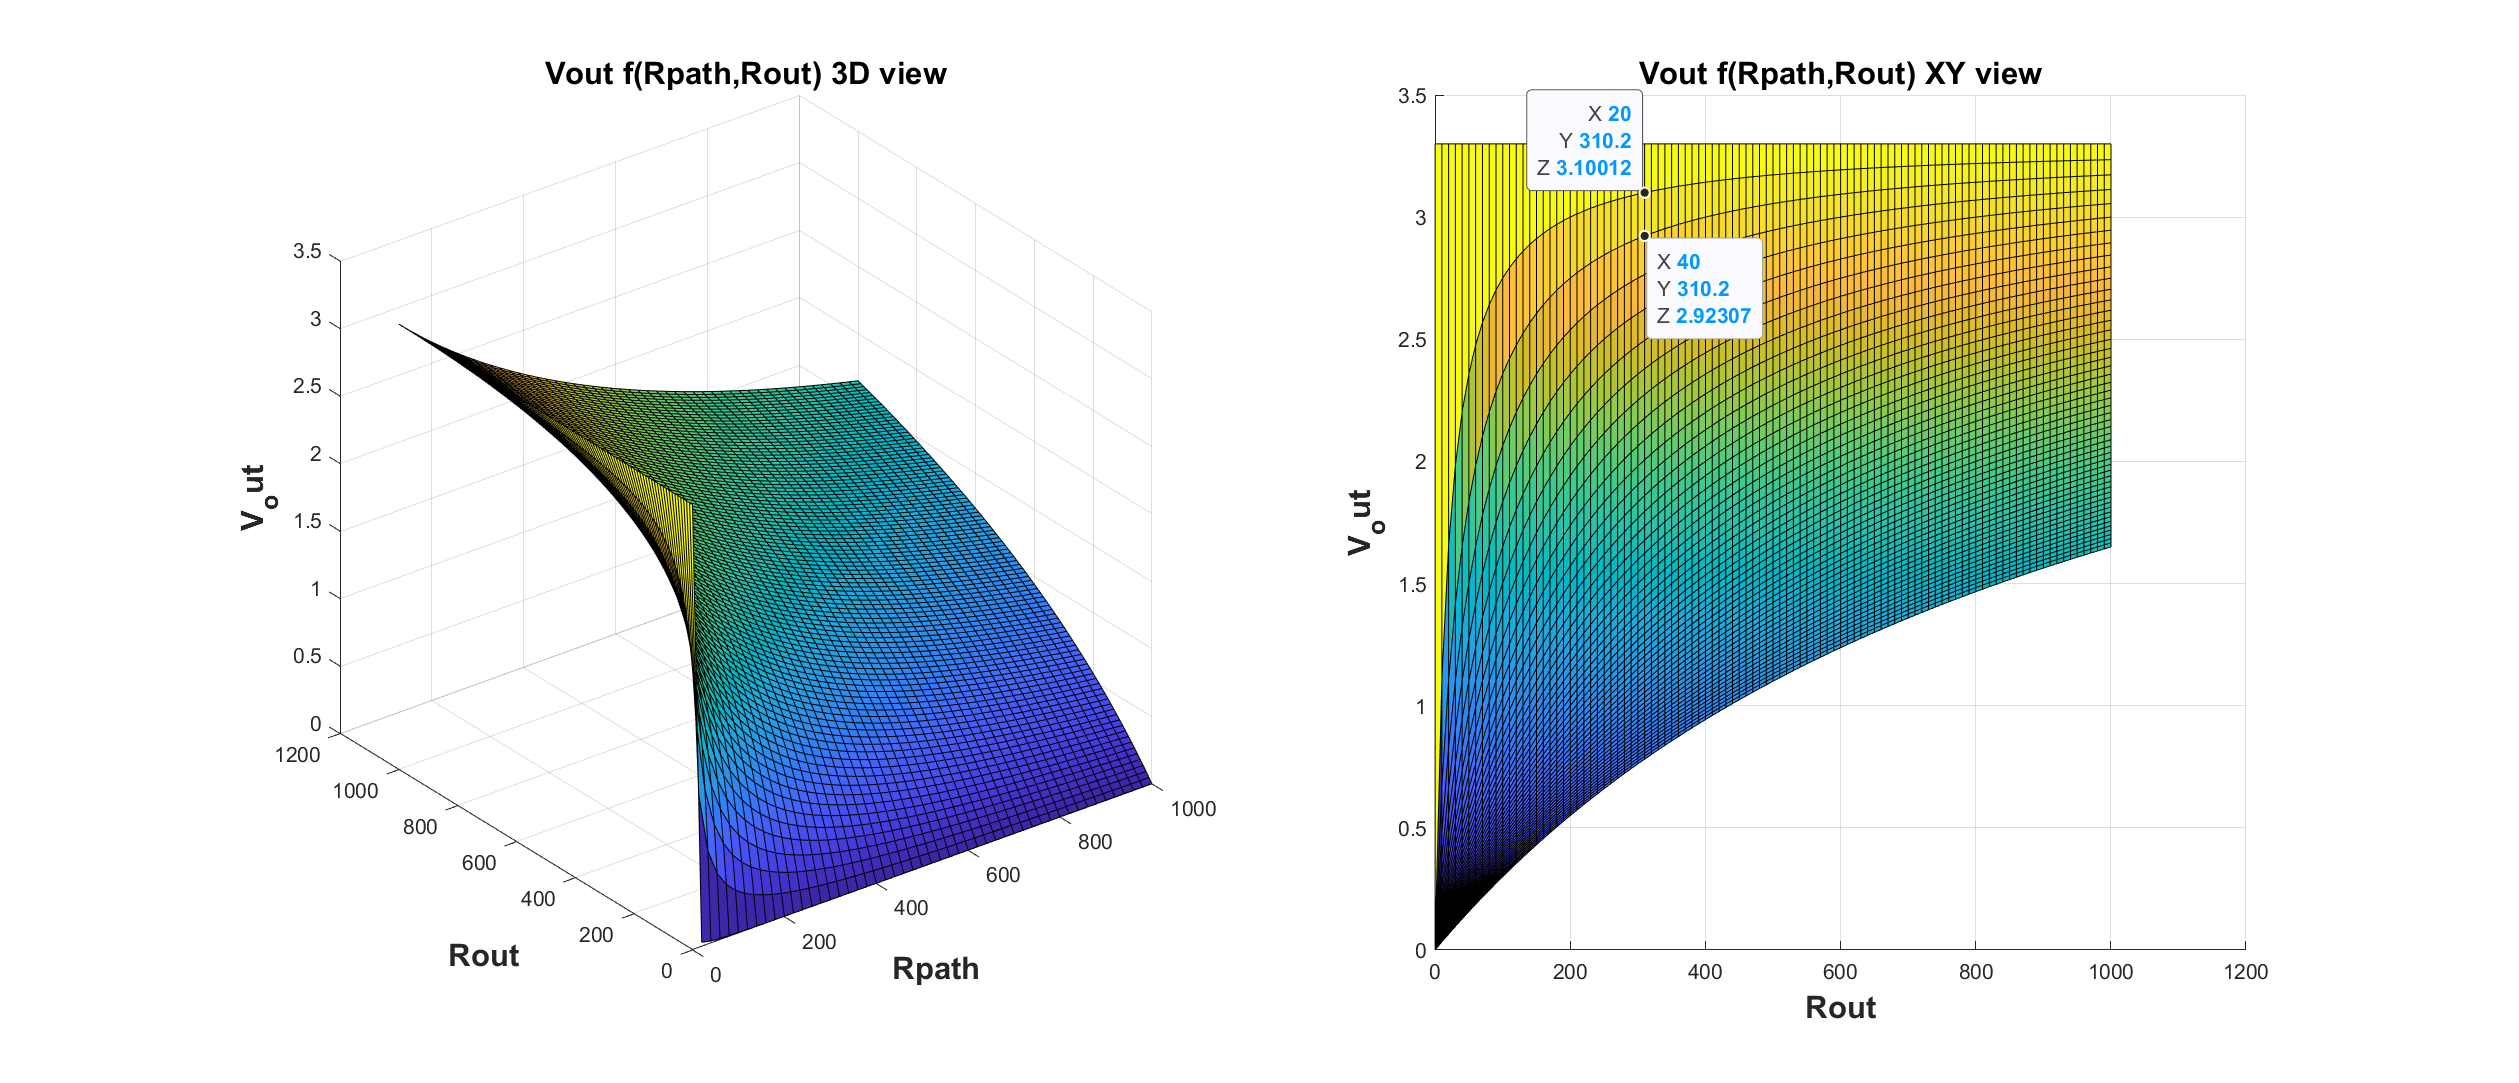
\includegraphics[width = 1\textwidth]{obrazky/Vout3D.eps}
    \caption{3D zobrazení rovnice pro výstupní napětí děliče (generováno pomocí MATLAB) }
    \label{fig:3D zobrazení rovnice pro výstupní napětí děliče}
\end{figure}

Nyní přejděme k řešení rovnice (\ref{eq:citilivost}). Následující obrázek \ref{fig: zobrazení df/dRpath}
zobrazuje ve své levé části zeleně hodnotu citlivostí $\frac{ \Delta V_{out} }{\Delta R_{path}}$
v celém zkoumaném prostoru. Červeně je pak zobrazena druhá strana rovnice (\ref{eq:citilivost}).
Podmínky jsou splněny ve všech kombinacích odporu $R_{out}$ a $R_{path}$, kde má zelená část
vyšší hodnoty diference než červená.
V pravé části obrázku je pro jednodušší odečítání hodnot odporu výsledné oblasti pohled "shora".
Zelená oblast splňuje podmínky a červená nesplňuje.
Obecně platí, čím hlouběji v zelené oblasti se zkoumaný bod nachází, tím vyšší je přesnost\\

\begin{figure}[ht!]
    \centering
    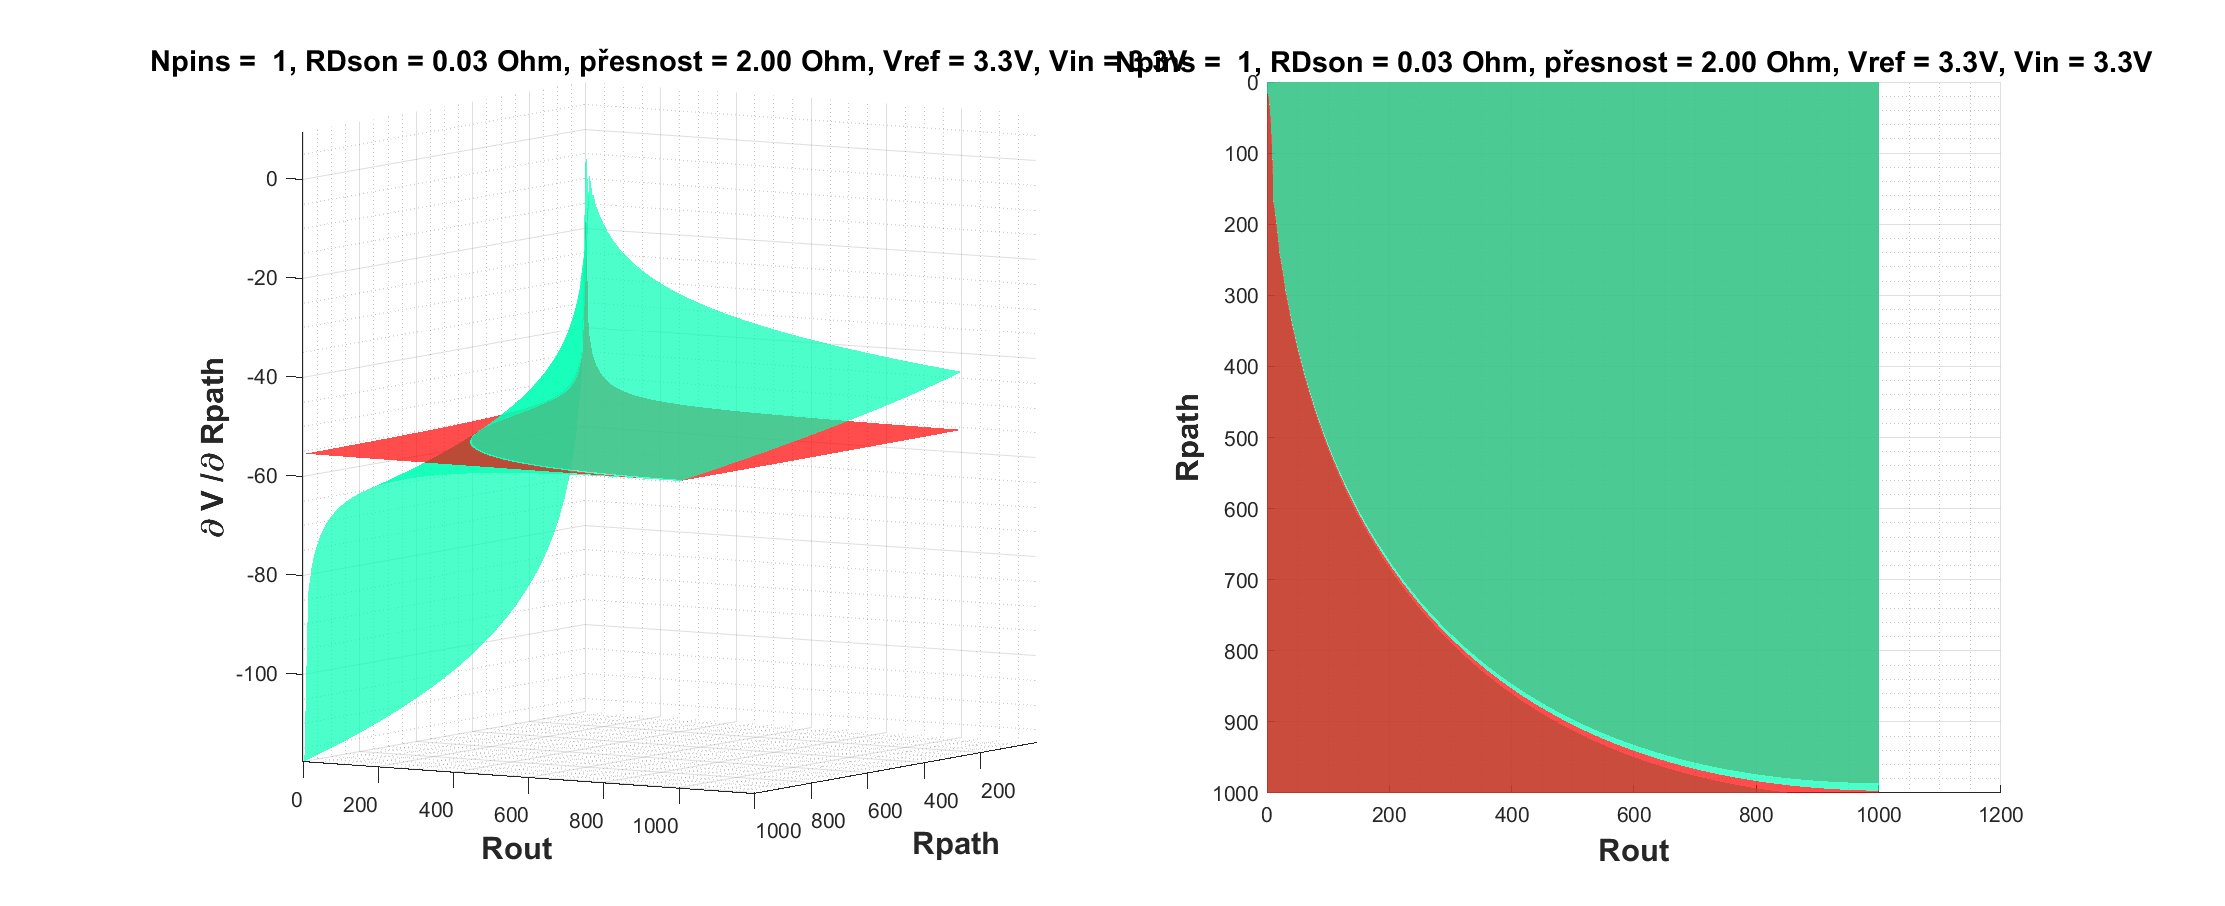
\includegraphics[width = 1\textwidth]{obrazky/general_dVF.eps}
    \caption{3D zobrazení rovnice \ref{eq:citilivost} s podmínkami (generováno pomocí MATLAB)}
    \label{fig: zobrazení df/dRpath}
\end{figure}

Do rovnice však vstupují parametry, jako je počet paralelně měřených pinů,
odpor $R^P_{DSon}$ a volba přesnosti. Následující série grafů zobrazuje vliv
těchto parametrů na výslednou oblast, která splňuje podmínky.
Výsledný zvolený odpor je 400$\Omega$ a v grafech jsou krajní hodnoty pro tento bod označeny
(x: $R_{path}$, y: $R_{out}$ a  z: $20log(\left| \frac{\partial V_{out} }{\partial R_{path}}\cdot \Delta R_{path} \right|$) ).\\
\clearpage

Zkoumání vlivu počtu pinů nás zajímá především při provozu testeru v PASS/FAIL režimu,
kdy je nutné provádět měření rychle. Zároveň zde máme definovanou maximální chybu měření
do 2$\Omega$. Při tomto testu se předpokládá, že všechny měřené cesty mají odpor do 100 $\Omega$.
Z obrázku \ref{fig:PASS_FAIL 2 OHMS MEASUREMENT} je patrné, že nebude možné
změřit všech 80 pinů jedné karty současně s požadovanou přesností.
Požadovanou přesnost nebude možné dosáhnout ani při měření 60 pinů současně, protože nejvyšší hodnota odporu cesty,
která leží v zelené oblasti je přibližně 60\, $\Omega$.
Při této úvaze bylo počítáno s $R^P_{DSon} = 0.03\Omega$, což je hodnota o cca 15m$\Omega$ vyšší než má použitý P - channel mosfet.
(Výběr mosfetu je dále v diplomové práci).
Hodnota zvoleného odporu 400$\Omega$ umožňuje,při měření 40 pinů současně, splnit podmínku přesnosti $\pm 2\Omega$ pro určení hodnoty odporu propojení do přibližně 220
$\Omega$.\\



\begin{figure}[ht!]
    \centering
    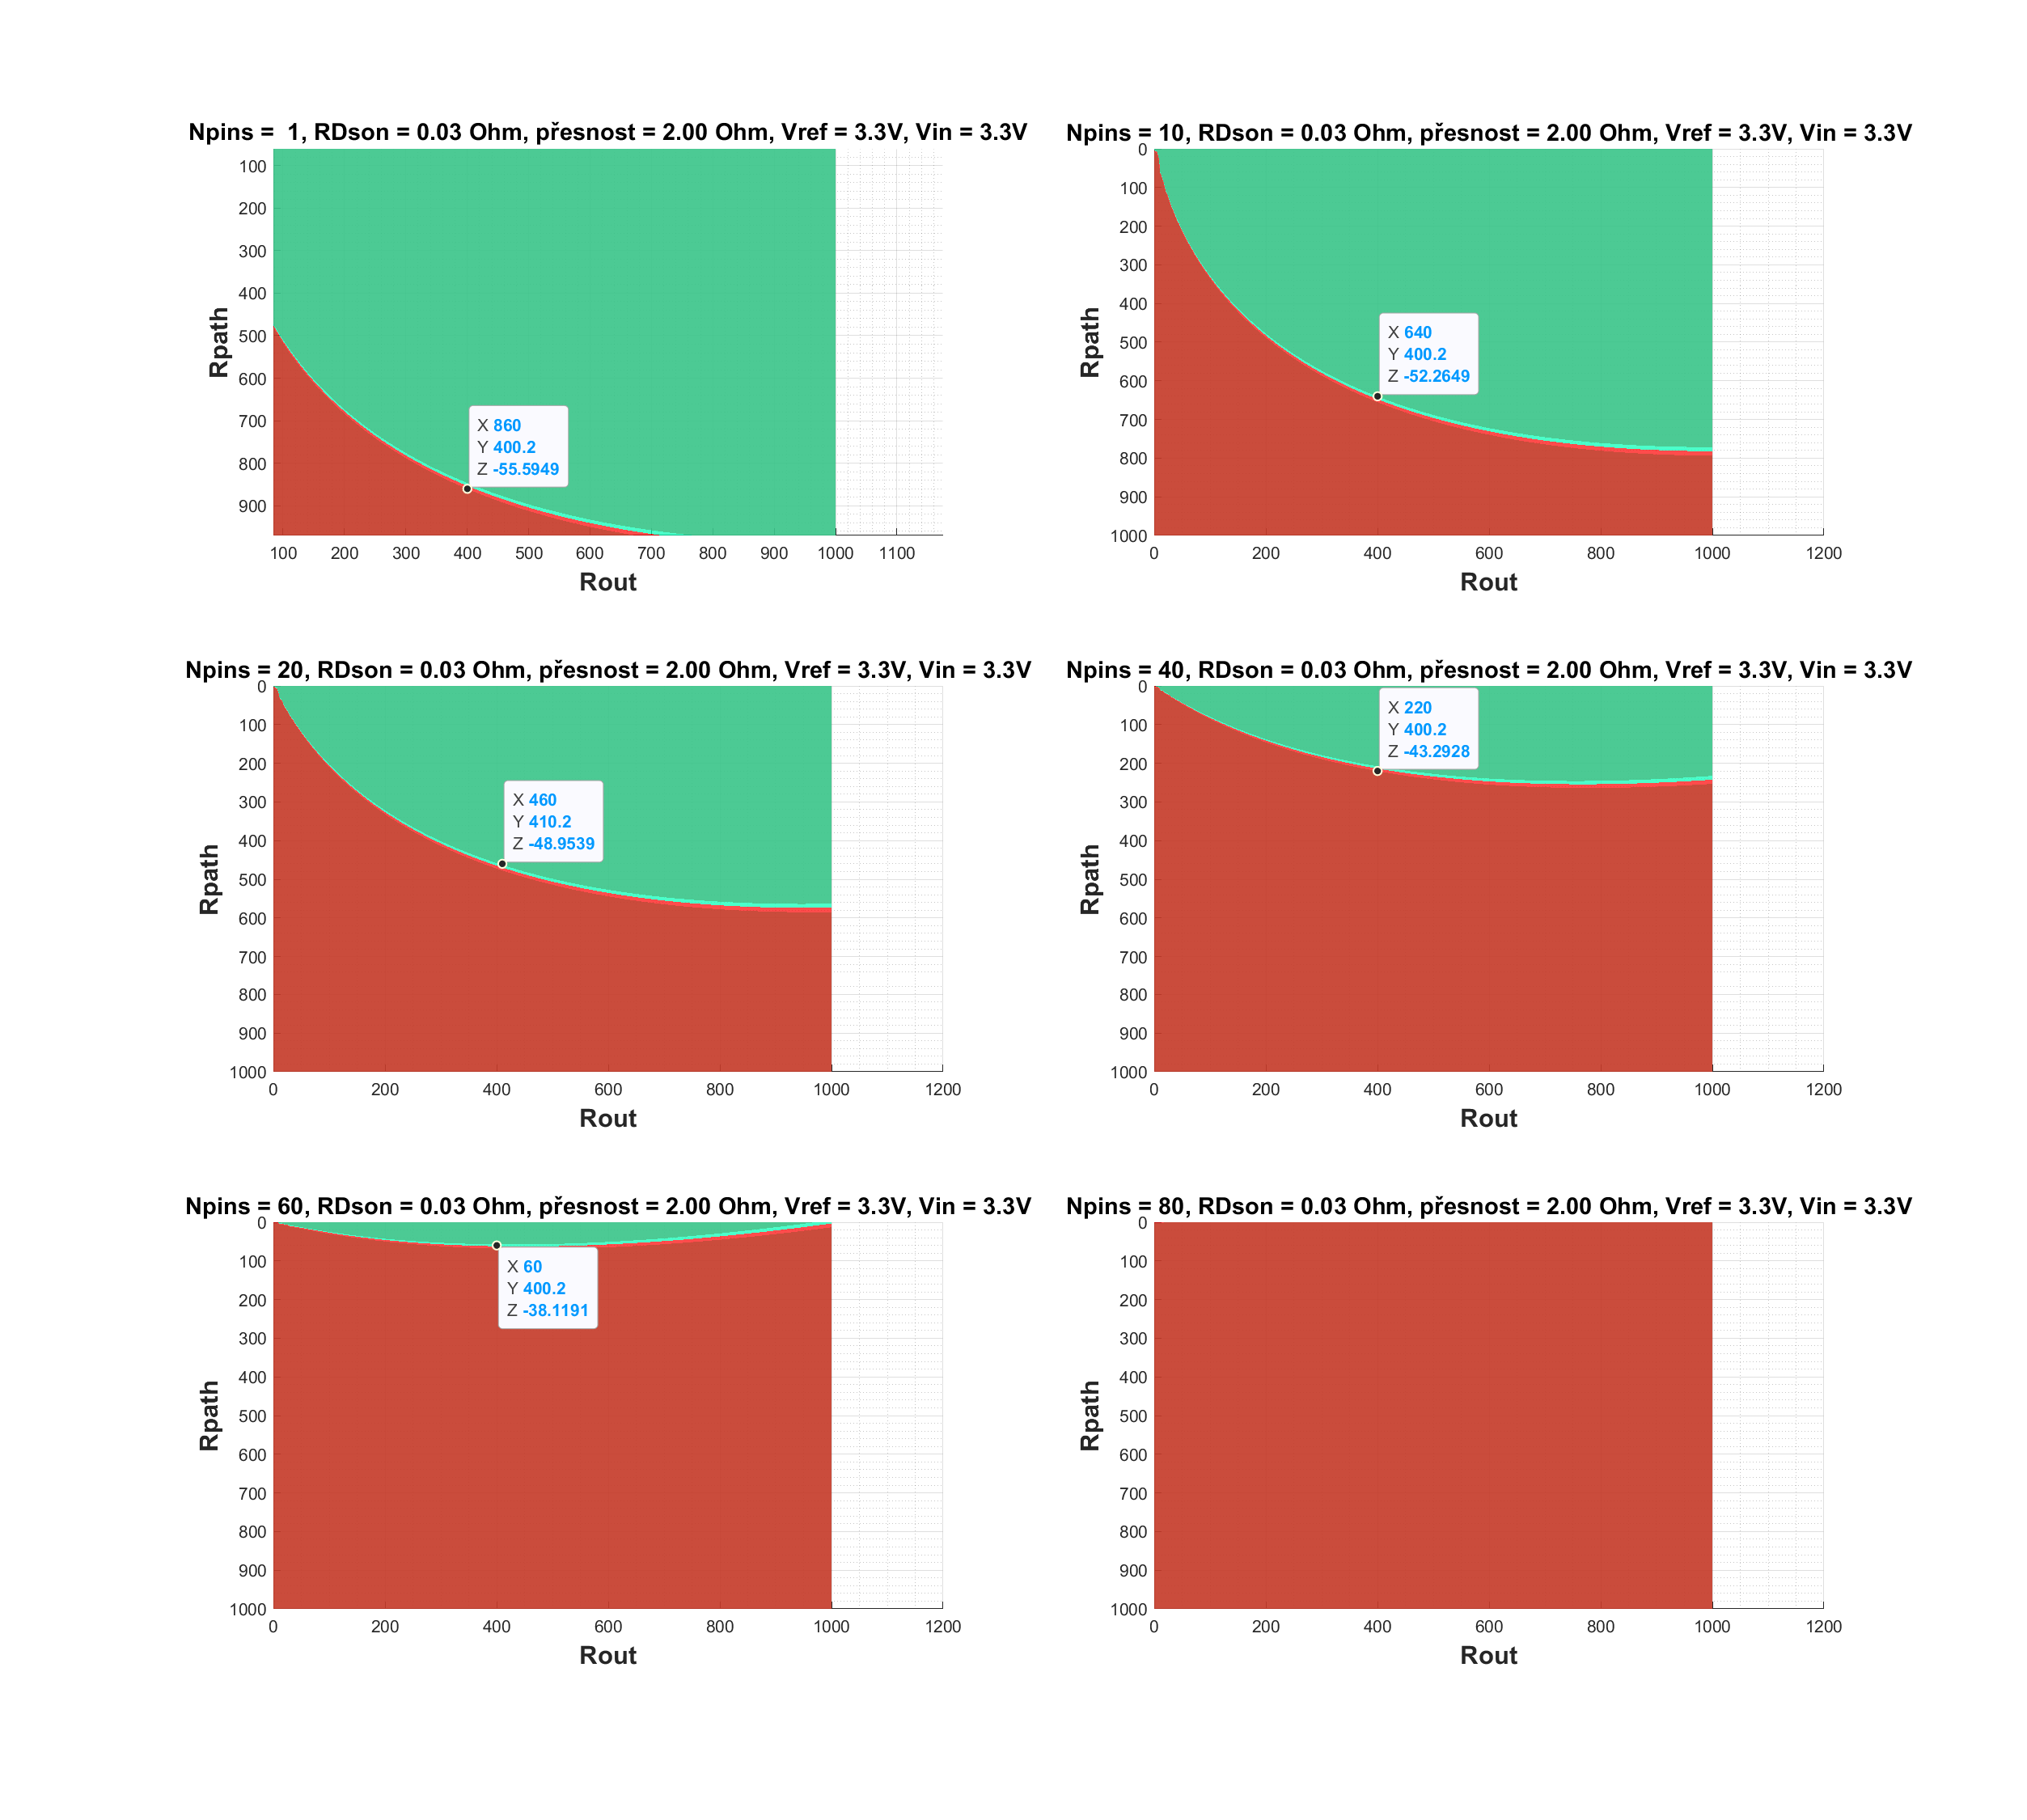
\includegraphics[width = 1\textwidth]{obrazky/PASS_FAIL_MERENI.eps}
    \caption{PASS FAIL -  přesnost $R_{path}$ 2$\Omega$ (generováno pomocí MATLAB)}
    \label{fig:PASS_FAIL 2 OHMS MEASUREMENT}
\end{figure}

\clearpage
Vliv požadované přesnosti měření nás zajímá v režimu vyhodnocení co nejpřesnější hodnoty měřené cesty.
V tomto režimu se předpokládá měření propojení pouze 2 pinů.
Z obrázku \ref{fig:One pin MEASUREMENT} je patrné, že vyšší přesnosti lze docílit volbou nižšího odporu $R_{out}$.
Tento požadavek je protichůdný s požadavkem na velikost odporu pro PASS/FAIL test(\ref{fig:PASS_FAIL 2 OHMS MEASUREMENT}).
Hodnota výsledného odporu 400$\Omega$ tak byla zvolena jako jistý kompromis mezi těmito dvěma požadavky.

\begin{figure}[ht!]
    \centering
    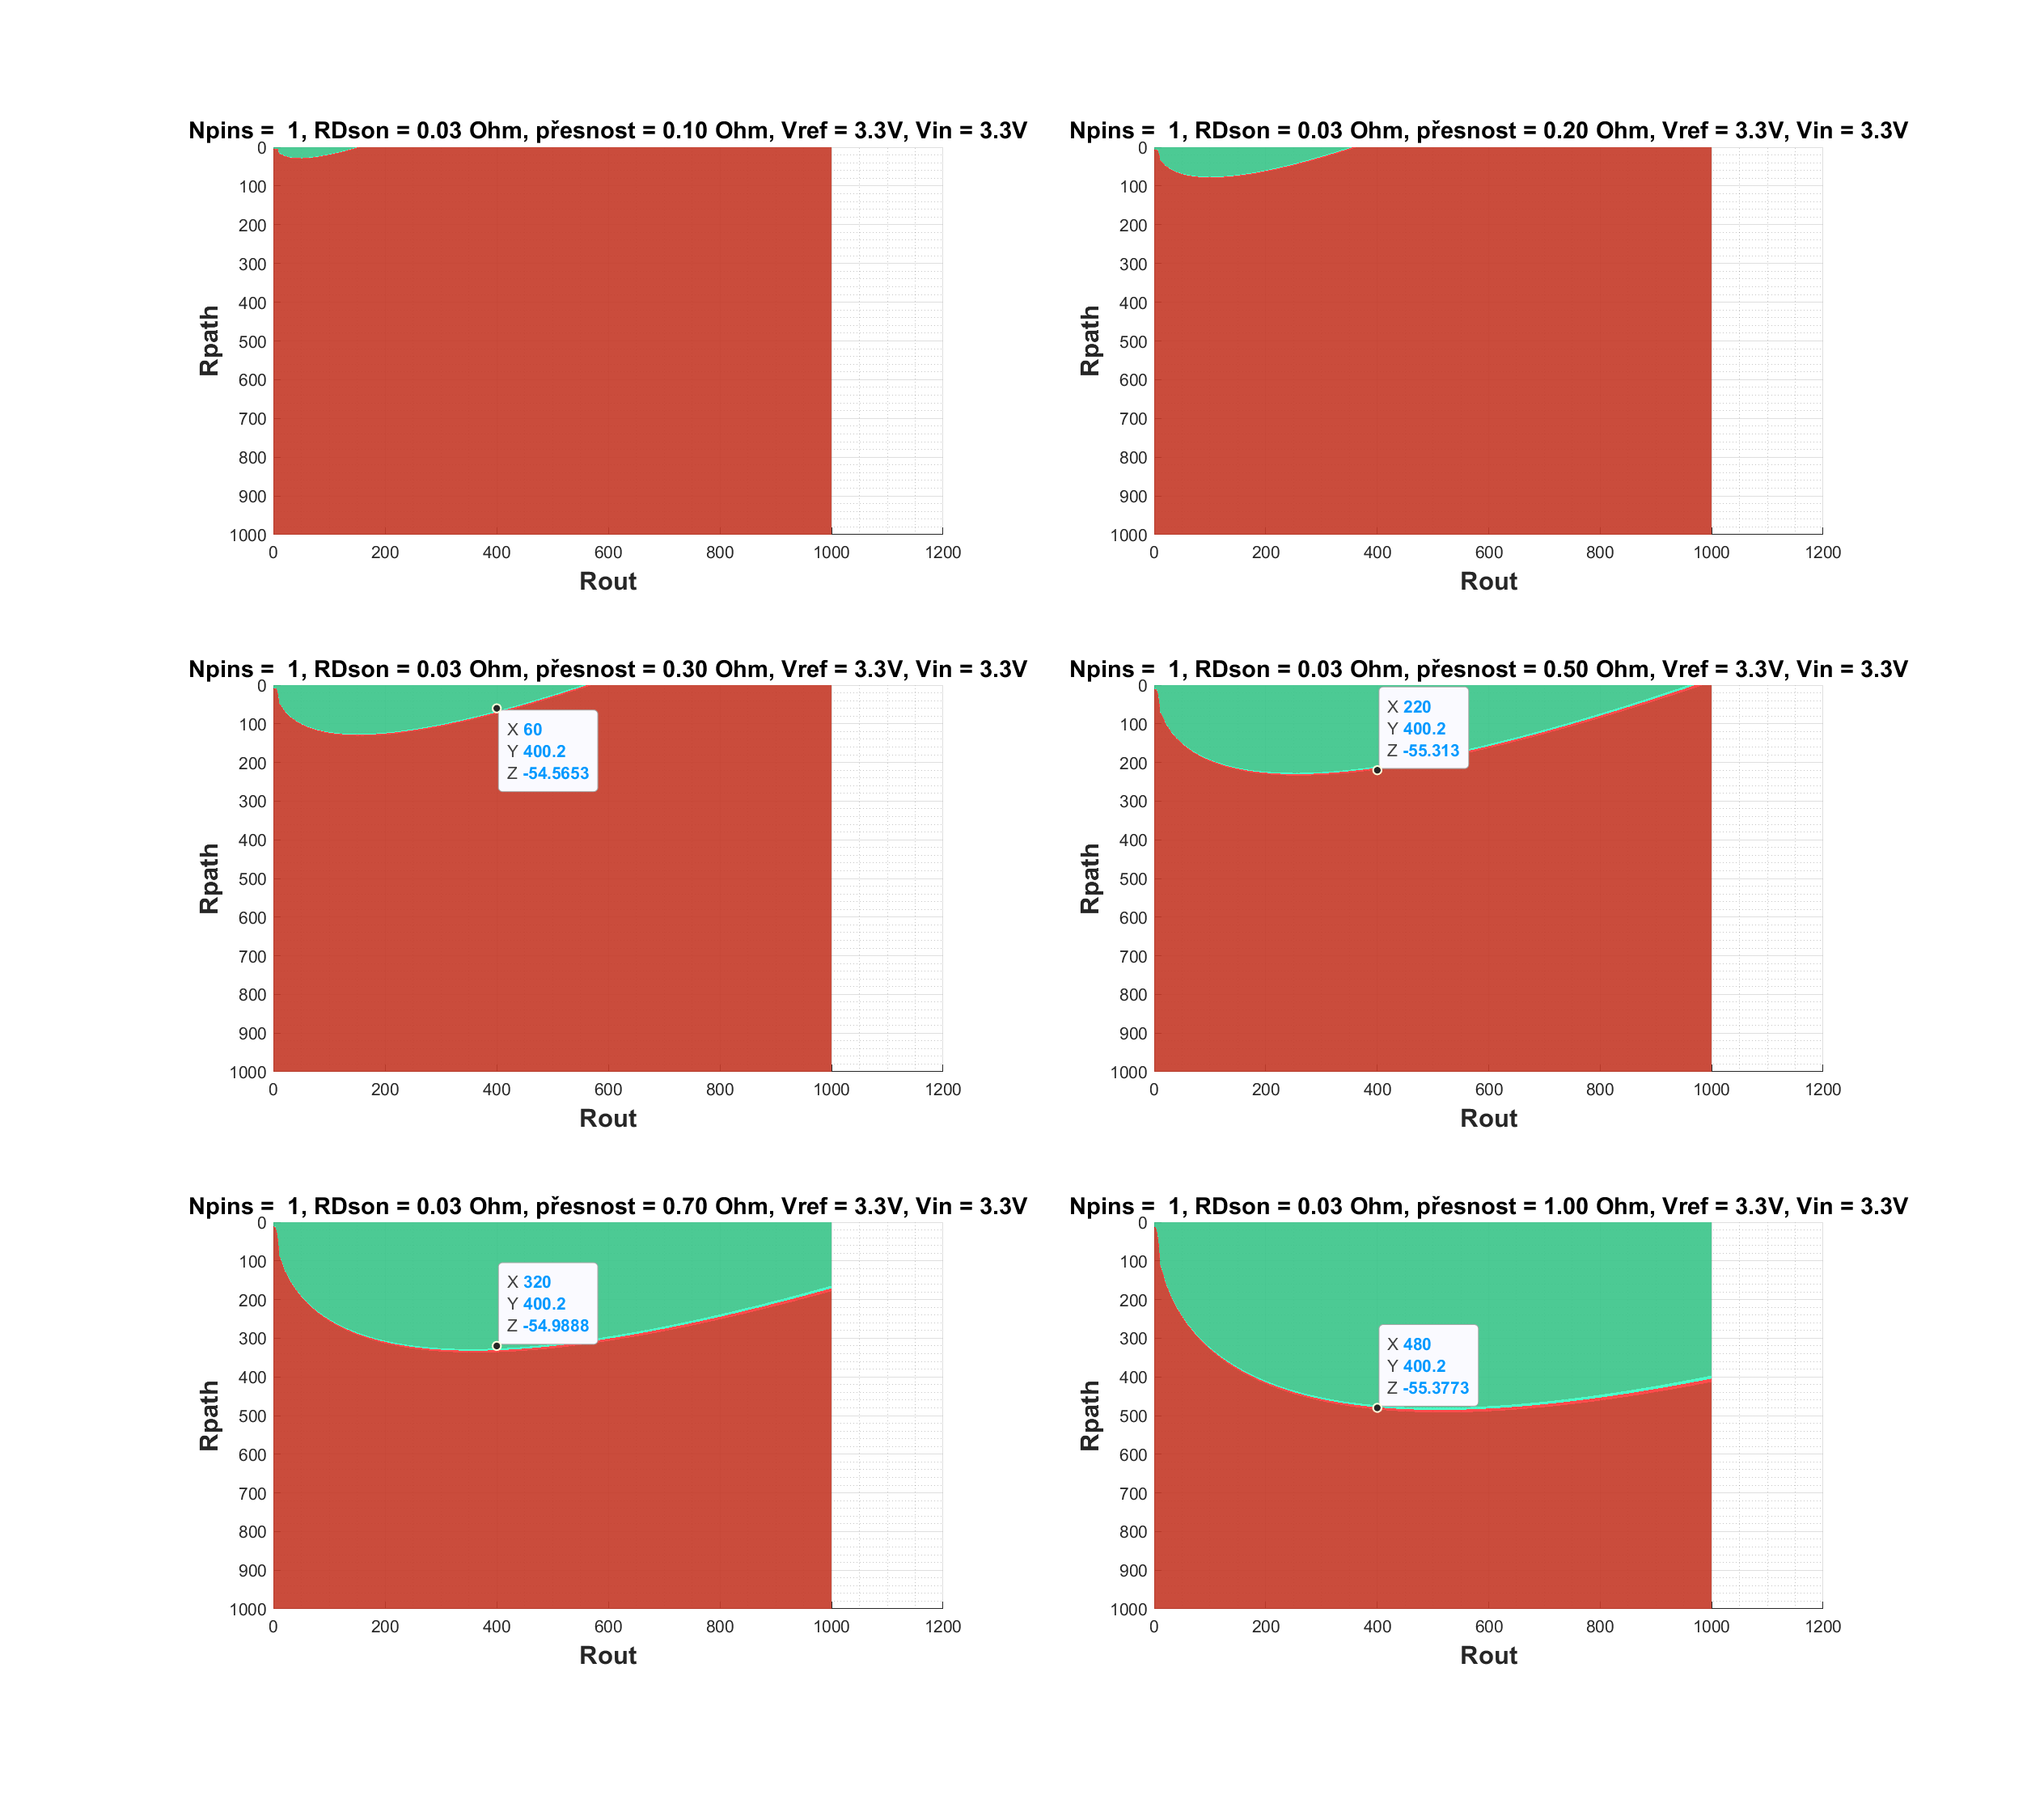
\includegraphics[width = 1\textwidth]{obrazky/MERENI_JEDNOHO_PINU.eps}
    \caption{Přesné měření mezi 2 piny - (generováno pomocí MATLAB)}
    \label{fig:One pin MEASUREMENT}
\end{figure}
\clearpage



\subsubsection{Volba P-channel mosfetu}
Při výběru P-channel mosfetu je vzhledem k podmínkám na přesnost nutné zvolit mosfet s nízkým odporem $R^P_{DSon}$.
Tohoto odporu by mělo být možno dosáhnout pomocí řídícího napětí 3.3V.
Zároveň by měl mosfet být schopen dodat do obvodu dostatečný proud pro měření 40 pinů současně (proč 40 pinů je zdůvodněno v kapitole
o volbě odporu $R_{out}$). Mosfet musí tedy do obvodu být schopen dodat následující minimální proud.

\begin{equation} \label{eq:MIN_CURRENT}
    I_{min} = \frac{40 \cdot V_{in}}{R_{out}} = \frac{40 \cdot 3.3}{400} = 330mA
\end{equation}

 Z následujícího obrázku je patrné, že při použití $R_{out} = 400\Omega$ je pro splnění podmínky přesnosti měření 2$\Omega$ v rozsahu od 1 do 100$\Omega$ zvolit mosfet s
 nejvyšším možným $R^P_{DSon}$ přibližně 0.032$\Omega$. Zároveň je zde požadavek na co nejnižší cenu, dostupnost a menší velikost pouzdra. 

\begin{figure}[ht!]
    \centering
    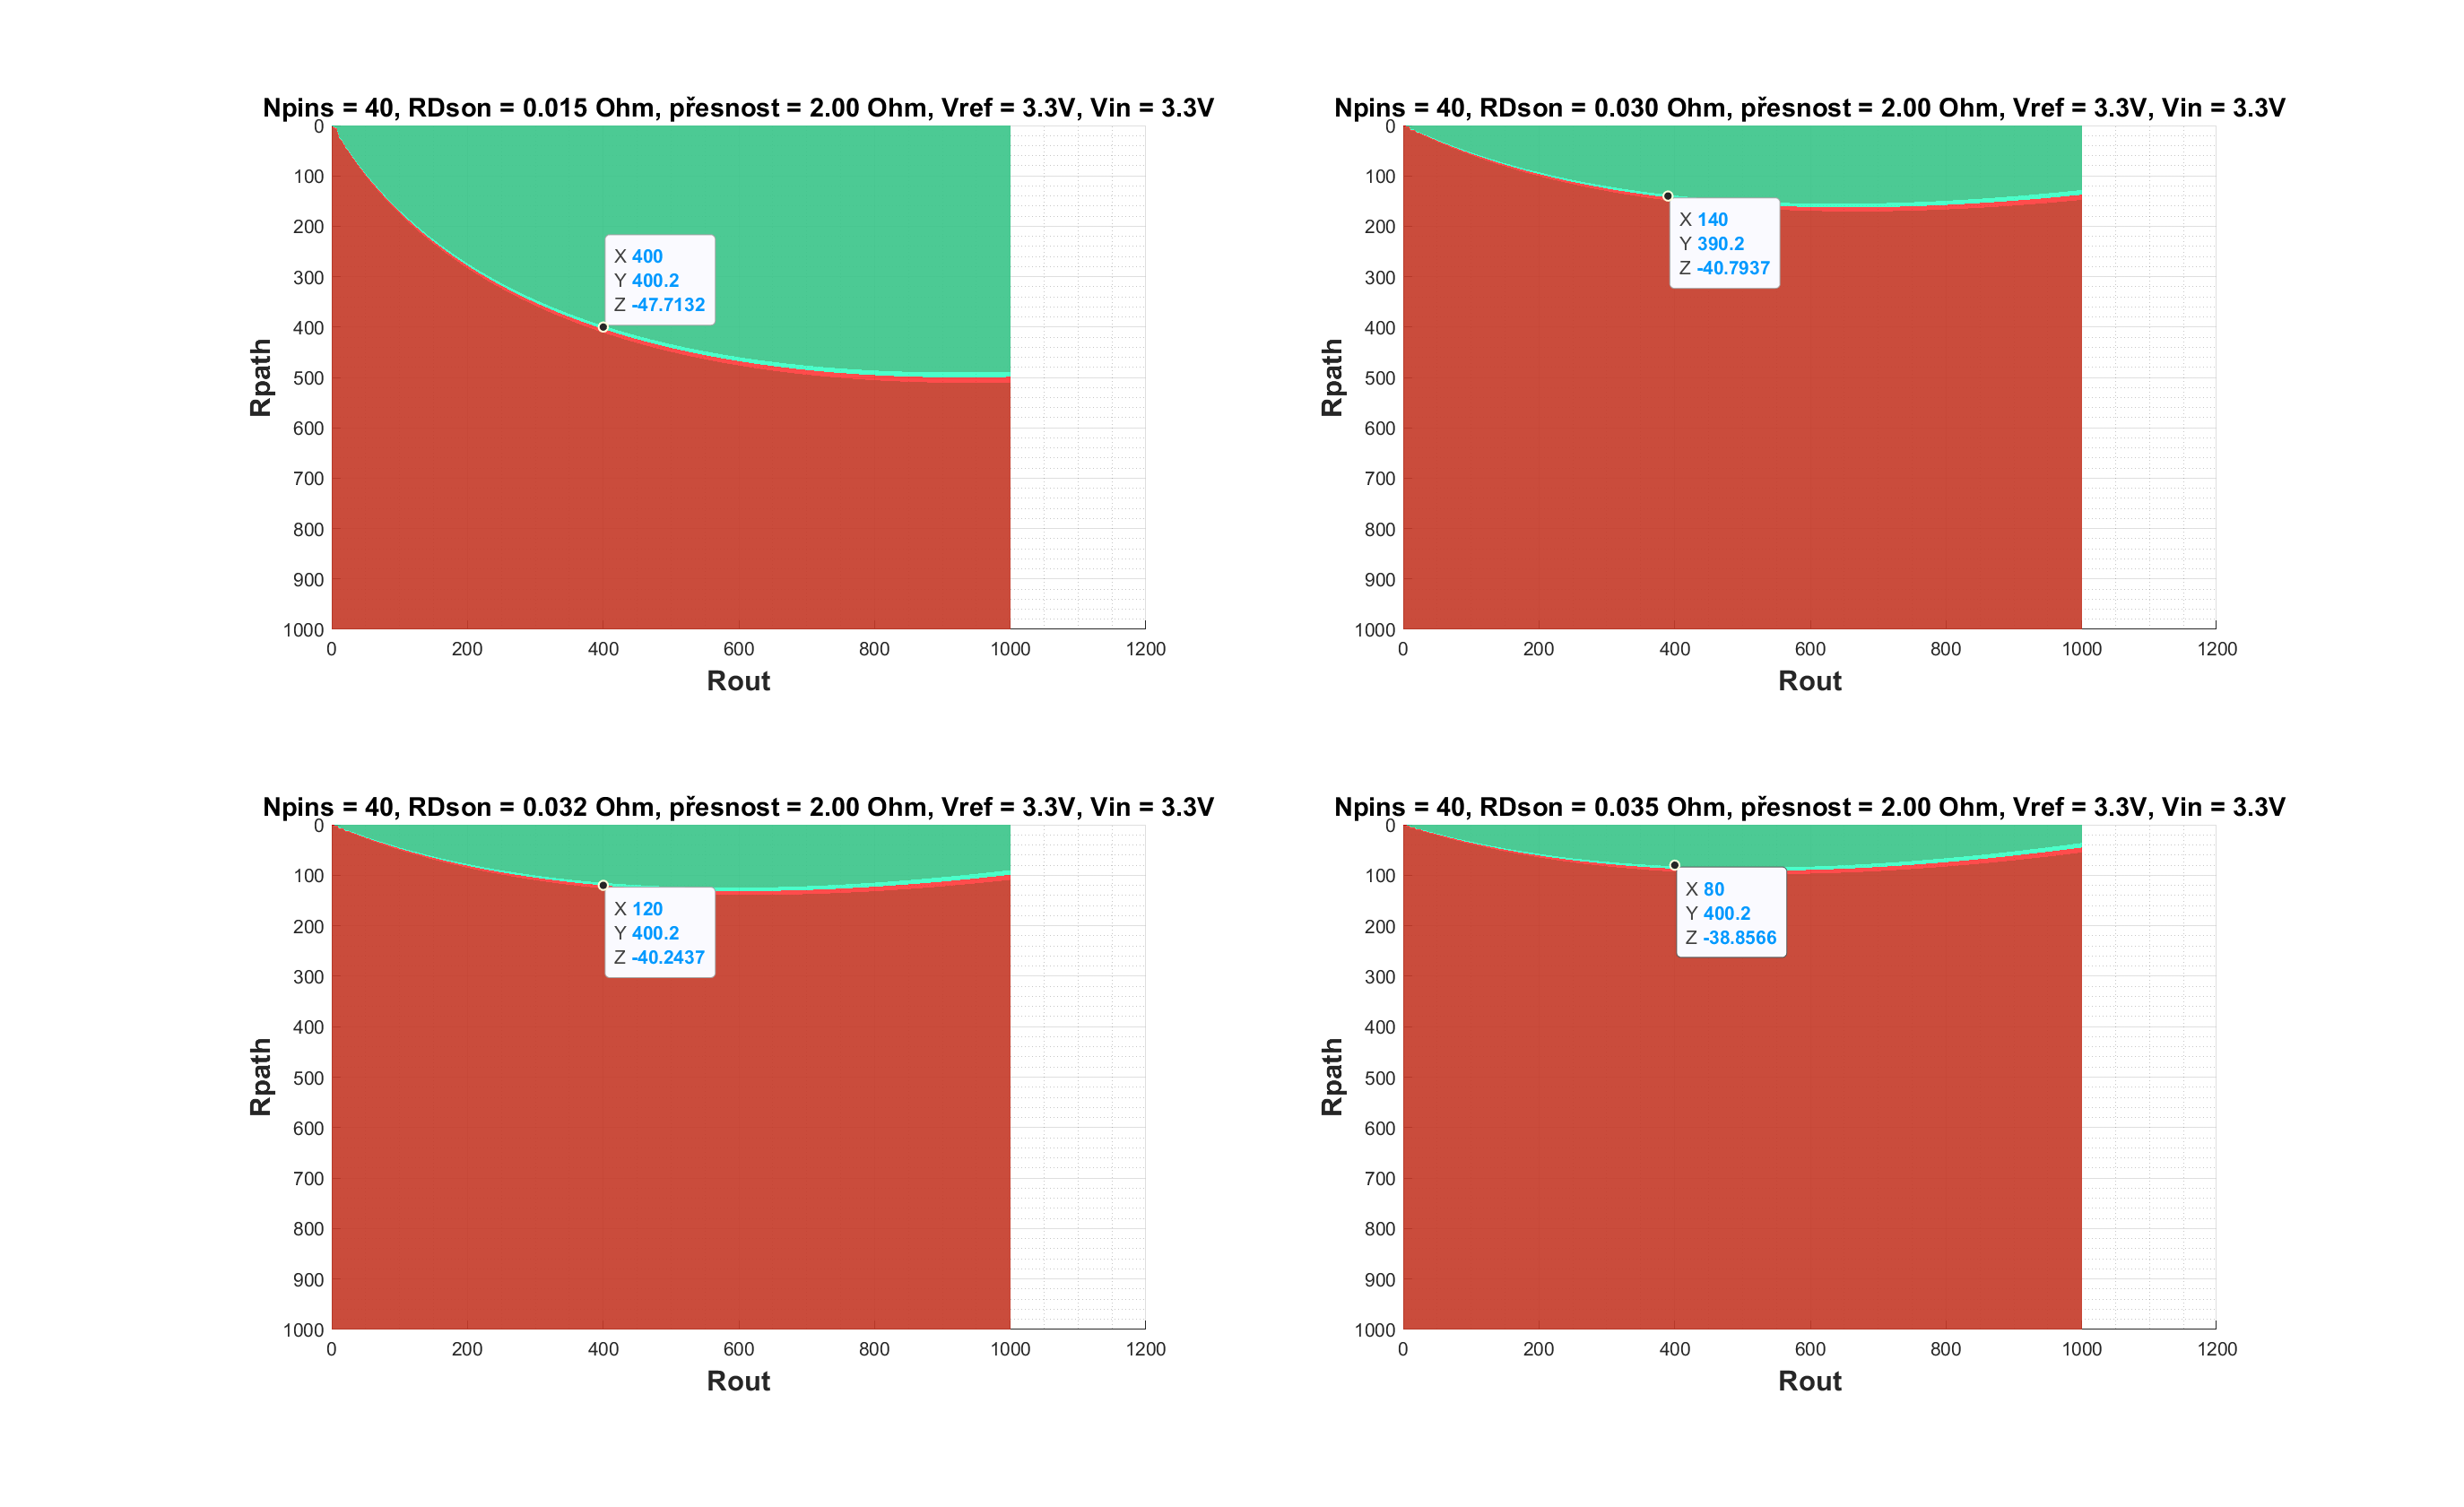
\includegraphics[width = 1\textwidth]{obrazky/vliv_RDSON.eps}
    \caption{vliv RDSon na přesnost měření (generováno pomocí MATLAB)}
    \label{fig:vliv RDSon}
\end{figure}

Na základě výše zmíněným požadavků byl zvolen mosfet SSM3J358R,LF. Níže je výstřižek z datasheetu. Podle typických hodnot by se mělo
docílit $R_{DSon}$ do 25\,m$\Omega$.
\begin{figure}[ht!]
    \centering
    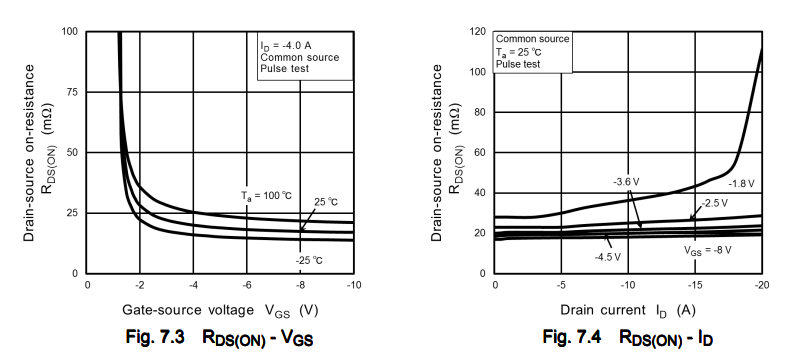
\includegraphics[height = 0.15\textheight]{obrazky/mosfet_datasheet.png}
    \caption{Výstřižek z datasheetu mosfetu SSM3J358R,LF - RDSON\cite{PMOS_datasheet}}
    \label{fig:Výstřižek z datasheetu mosfetu SSM3J358R,LF - RDSON}
\end{figure}

\clearpage

\subsubsection{Volba N-channel mosfetu}
Parametry N-channel mosfetu nemají příliš velký vliv na chování obvodu, protože jeho odpor $R^N_{DSon}$ je započítán do hodnoty odporu $R_{out}$.
Zároveň je hodnota $R^N_{DSon}$ většinou nižší než tolerance odporu $R_{out}$. Hlavním požadavkem je zde, aby bylo možno ovládat mosfet 3.3 a 5V logikou.
Dále by měl mosfet být schopen snést proud I = 3.3/400 = 8.25mA, byl co nejlevnější dostupný a měl menší velikost pouzdra. Byl vybrán PJA3432\_R1\_00001
s následujícími parametry.\\

\begin{figure}[ht!]
    \centering
    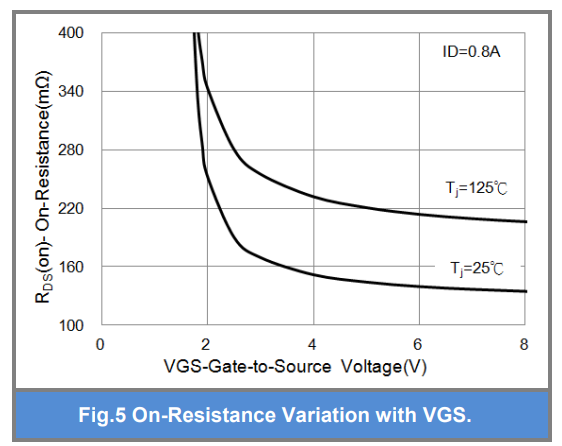
\includegraphics[height = 0.25\textheight]{obrazky/Nmosfet_datasheet.png}
    \caption{Výstřižek z datasheetu N-channel mosfetu PJA3432\_R1\_00001 - RDSON\cite{NMOS_datasheet}}
    \label{fig:Výstřižek z datasheetu N-channel mosfetu}
\end{figure}

\subsubsection{Volba komparátoru}
Doposud nebylo počítáno s vlivem reálného komparátoru.
Aby byly výsledky co nejpřesnější je vhodné zvolit komparátor s co nejvyšším vstupním odporem.
Protože při propojení pinů nízkou hodnotou odporu je výstupní napětí děliče blízké napájecímu napětí, tak je komparátor
napájen vyšším napájecím napětím konfigurovatelným od cca 4 do 5.5V (více v sekci o napájení).
Komparátor by také neměl mít hysterzi. Dále, protože je vstup komparátoru přímo připojen
na bRC piny, tak by zde měla být ESD ochrana.\\

Pro jednodušší PCB layout je vhodné, aby pouzdro obsahovalo více komparátorů.
Co se týče input voltage offsetu, tak na jeho velikosti
příliš nezáleží, protože bude minimalizován kalibrací. Offset by však měl být stabilní.\\

Byl vybrán komparátor LM393LVQDRQ1. Vstup komparátoru je interně chráněn proti ESD do 2kV.
Na výstupu komparátoru je pull-up rezistor připnutý k napájení
ovládací karty (tímto je docíleno napěťové kompatibility s 3V3 i 5V logikou).
Vybraný komparátor má poměrně vysokou kapacitu vstupu (3\,pF).
Vliv kapacity je diskutován v sekci o návrhu D/A převodníku ovládací karty\cite{comp_datasheet}.


\subsubsection{Volba shift registrů}
Základním požadavkem na shift registry je možnost řízení pomocí 3V3 logiky, přičemž shift registr samotný je napájen 5V.
Dále schopnost řídit vybrané P a N-Channel mosfety. Všech 80 výstupů (P-Mosfetů) je řízeno 2x5 shift registry zapojených do série.
Pro výstupní piny není kladen velký důraz na rychlost nastavení hodnot,
protože pro každý výstupní pin je nutné změřit dalších 4000 vstupních tak je na přepínání času dostatek.
Naopak ovládání N-channel mosfetů by mělo být co nejrychlejší.\\

V kapitole o výběru rezistoru děliče je zmíněno, že bude možné měřit 40 pinů současně.
Jistým kompromisem jednoduchosti ovládání a rychlostí je tak ovládat N-channel mosfety 10 shift
registry zapojenými stylem 2x5 do série (viz. schéma měřící karty v příloze).\\

Toto řešení ovládání je zároveň modulární, lze odebírat celé bloky po 8 pinech a
zlevnit tak měřící kartu pro použití v jednodušších aplikacích. Stejně jako u předchozích součástek i zde
je požadavek na menší pouzdro. Byl vybrán shift registr SN74AHCT595PWR.
Tento shift registr je 3 stavový, lze tak přímo řídit jednotlivé mosfety bez nutnosti
pull-up/down rezistorů. Poblíž napájení každého z shift registrů je umístěn 100nF vazební kondenzátor.
Řídící piny shift registrů jsou přivedeny na 2x25 pinový konektor,
kterým je měřící deska připojena k ovládací desce\cite{shift_datasheet}.

\subsubsection{Volba multiplexerů}
Multiplexer by měl být ovladatelný 3.3V i 5V logikou. Byl zvolen multiplexer\\ TMUX1308QDYYRQ1.
K multiplexeru je obdobně jako k shift registru připojen 100nF vazební kondenzátor.
Komparátory jsou zapojeny stylem 2x5 a mají jednotnou adresaci (2x3 adresní piny, 2x enable pin, 2x5 výstupních pinů).
Výstupy multiplexeru jsou přivedeny na 2x25 pinový konektor\cite{mux_datasheet}.

\clearpage

\subsection{Napájecí část}
Měřící karta je ve svém
standardním provedení napájena 7V až 15V.
Toto napájecí napětí je následně regulováno
dvěma nastavitelnými regulátory TLV76701DGNR na 3V a 5V .
Tyto regulátory disponují enable pinem, kterým je možné spínat regulátory ve správném pořadí,
tak aby nedocházelo k nedefinovaným stavům. Enable piny jsou řízeny pomocí ovládací karty, je však možno
pomocí jumperů přepnout regulátory do režimu, kde se spínají současně automaticky.
Dále tyto regulátory nabízí výstupní proud až 1A, ESD ochranu vstupů a automatickou tepelnou ochranu.\cite{regulator_datasheet}\\

\begin{figure}[ht!]
    \centering
    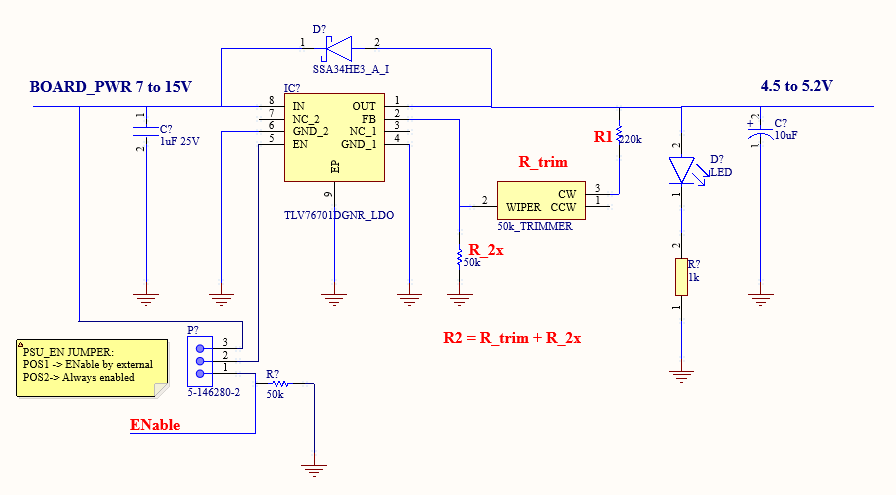
\includegraphics[width = 1\textwidth]{obrazky/PSU.png}
    \caption{Napájení měřící karty: 5V regulátor (celé schéma měřící karty v příloze -  POWER REGULATORS)}
    \label{Napájení měřící karty: 5V regulátor}
\end{figure}

Napětí 5V, ve finálním schématu v příloze označeno jako Vcomp,
slouží k napájení multiplexerů, komparátorů a shift registrů. Ve zpětnovazebním obvodu regulátoru
je připojen odporový dělič s 50\,k$\Omega$ trimmerem, pomocí kterého lze nastavit výstupní napětí v rozmezí
přibližně od 4.5 do 5.2V. Vzhledem k povaze napájených komponentů se nepředpokládá vysoký odběr proudu.\\

Napětí 3V, ve finálním schématu v příloze označeno jako Vpins, slouží k generování napětí na bRC pinech. Obdobně jako regulátor pro 5V má i regulátor pro 3V trimmer pro
nastavení výstupního napětí. Zde je však v napěťovém děliči zvolena jiná hodnota pevného rezistoru R1, tak aby
bylo možno pomocí 50\,k$\Omega$ trimmeru nastavit výstupní napětí v rozmezí od 2.8 do 3.5V.
Protože bude referenční napětí generováno 3.3V D/A převodníkem. Počítá se s nastavením výstupního napětí na 3V pro 
případ, že by převodník nefungoval v celém svém rozsahu. 3V regulátor musí být schopen dodat do obvodu proud minimálně
330mA (zdůvodnění je patrné z rovnice \ref{eq:MIN_CURRENT}).
Volba hodnot rezistorů ve zpětné vazbě vychází z rovnice pro výstupní napětí regulátoru
\begin{equation}
    V_{out} = V_{FB}  \cdot (1 + \frac{R1}{R2}),
\end{equation}

\noindent kde $V_{FB}$ = 0.8V, pro R2 byl použit 50\,k$\Omega$ trimmer v sérii s odporem 50\,k$\Omega$.
Hodnota R1 pro 5V regulátor byla zvolena
220\,k$\Omega$ a pro 3V regulátor 120\,k$\Omega$.\\

Regulátory mají připojeny shotky diody SSA34HE3. Tyto diody slouží jako ochrana proti přepětí na výstupu.
Na výstupu regulátorů jsou připojeny LED pro snadnou kontrolu, zda je regulátor zapnutý.
Výstupy regulátorů jsou přivedeny na jak na 2x25 pin konektor, tak na pole pinů pro připojení bRC (případně DIN konektoru).
Je tak možno využít výstupní napětí regulátorů pro napájení externích komponent, nebo
také regulátory neosazovat a napájet měřící kartu externím regulovaným zdrojem.\\

Na měřící kartě lze také nalézt napětí, které je ve finálním schématu v příloze označeno jako PWR\_MCU.
Toto napětí je do měřící desky přivedeno z ovládací karty. Je to napětí, které je následně využito
pro výstup multiplexerů (pull up výstupu komparátoru) a je tím zajištěna napěťová kompatibilita s ovládací logikou 3.3V a 5V.


\subsection{Návrh PCB}
Pro návrh PCB bylo využito softwaru Altium Designer. PCB bylo vyrobeno firmou
JLCPCB.
Jedná se o 6-ti vrstvé PCB s následujícím rozložením vrstev.
Jednotlivé vrstvy mají následující účel:
\begin{itemize}
    \item TOP layer: signal; polygon - GND
    \item inner layer 1: GND
    \item inner layer 2: signal; polygon - GND
    \item inner layer 3: signal/PWR; polygon - PWR\_MCU, Vref
    \item inner layer 4: PWR; polygon - BOARD\_PWR, Vpins, Vcomp
    \item BOTTOM layer: signal; polygon - GND, Vref
\end{itemize}

\noindent Za označením "polygon -"\ jsou uvedeny jména signálů, které mají v dané vrstvě nějaký polygon.
Následující obrázek zobrazuje všechny vrstvy současně bez polygonů. Na další straně jsou jednotlivé vrstvy
včetně polygonů.

\begin{figure}[ht!]
    \centering
    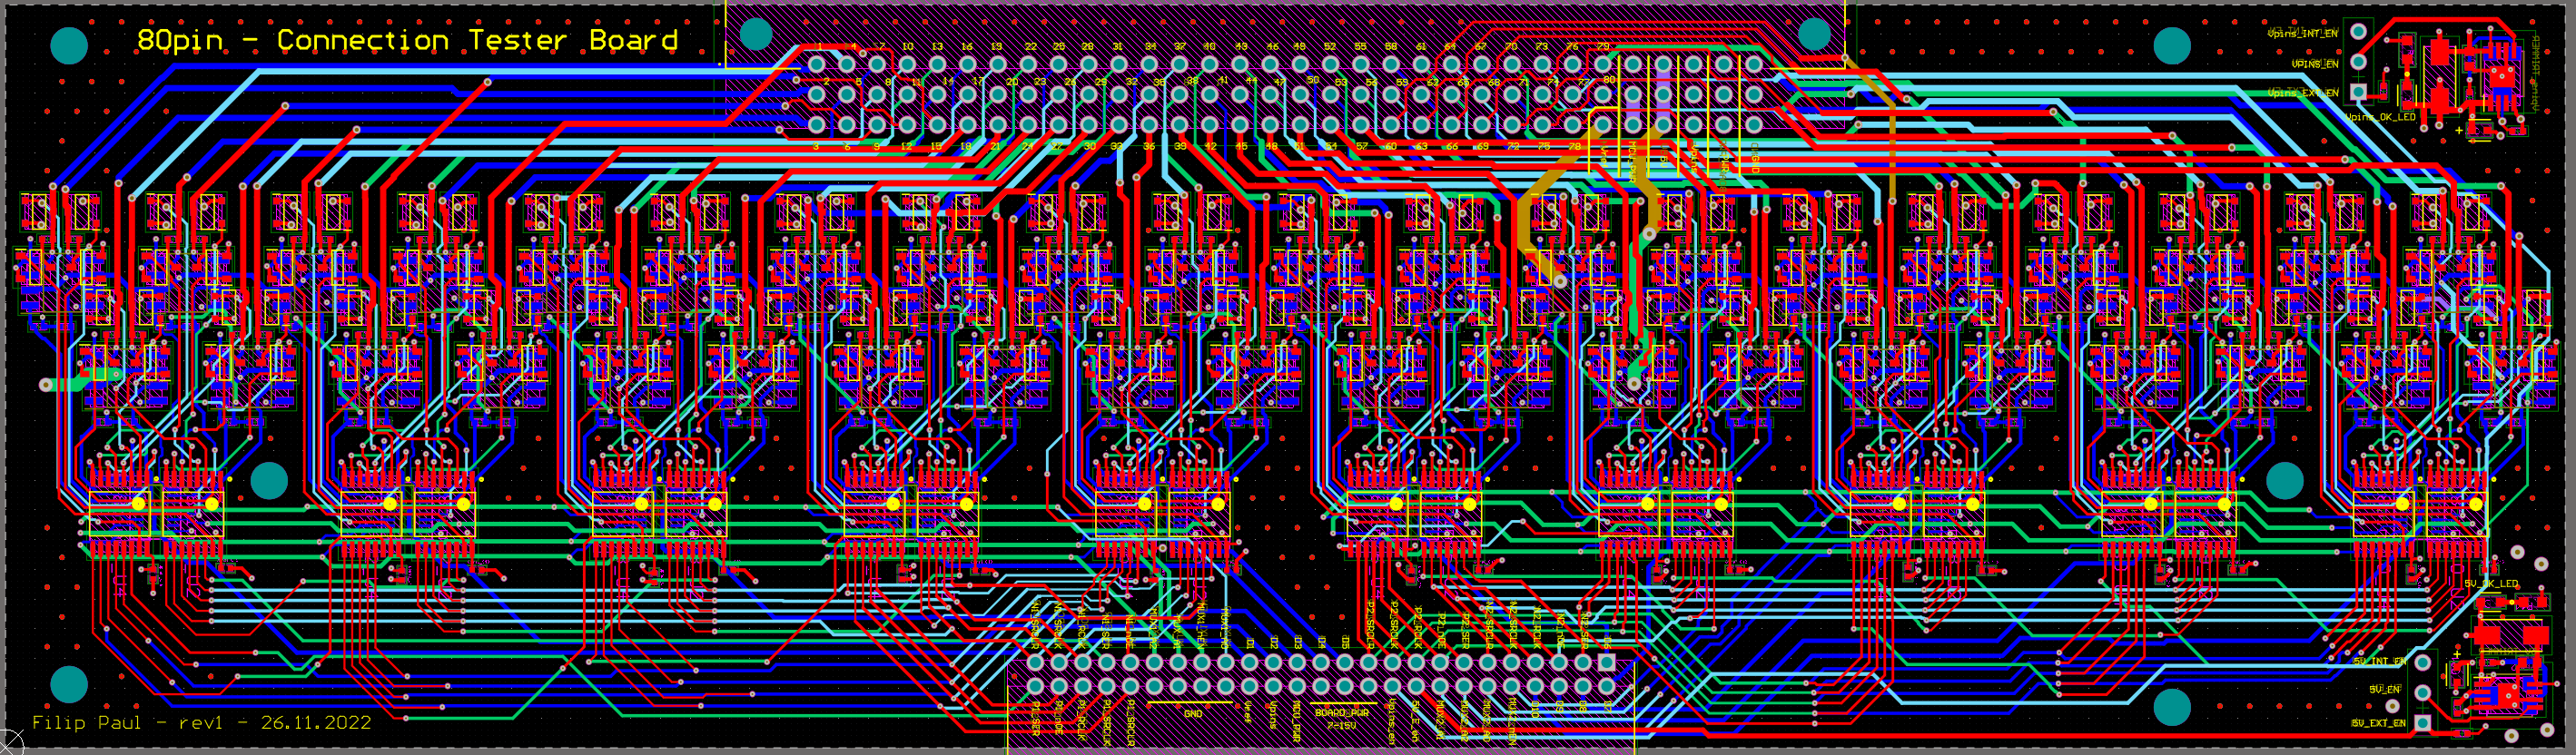
\includegraphics[width = 1\textwidth]{obrazky/all_layers_no_poly.png}
    \caption{Všechny vrstvy bez polygonů}
    \label{fig:Všechny vrstvy bez polygonů}
\end{figure}
\clearpage

\begin{figure}[ht!]
    \centering
    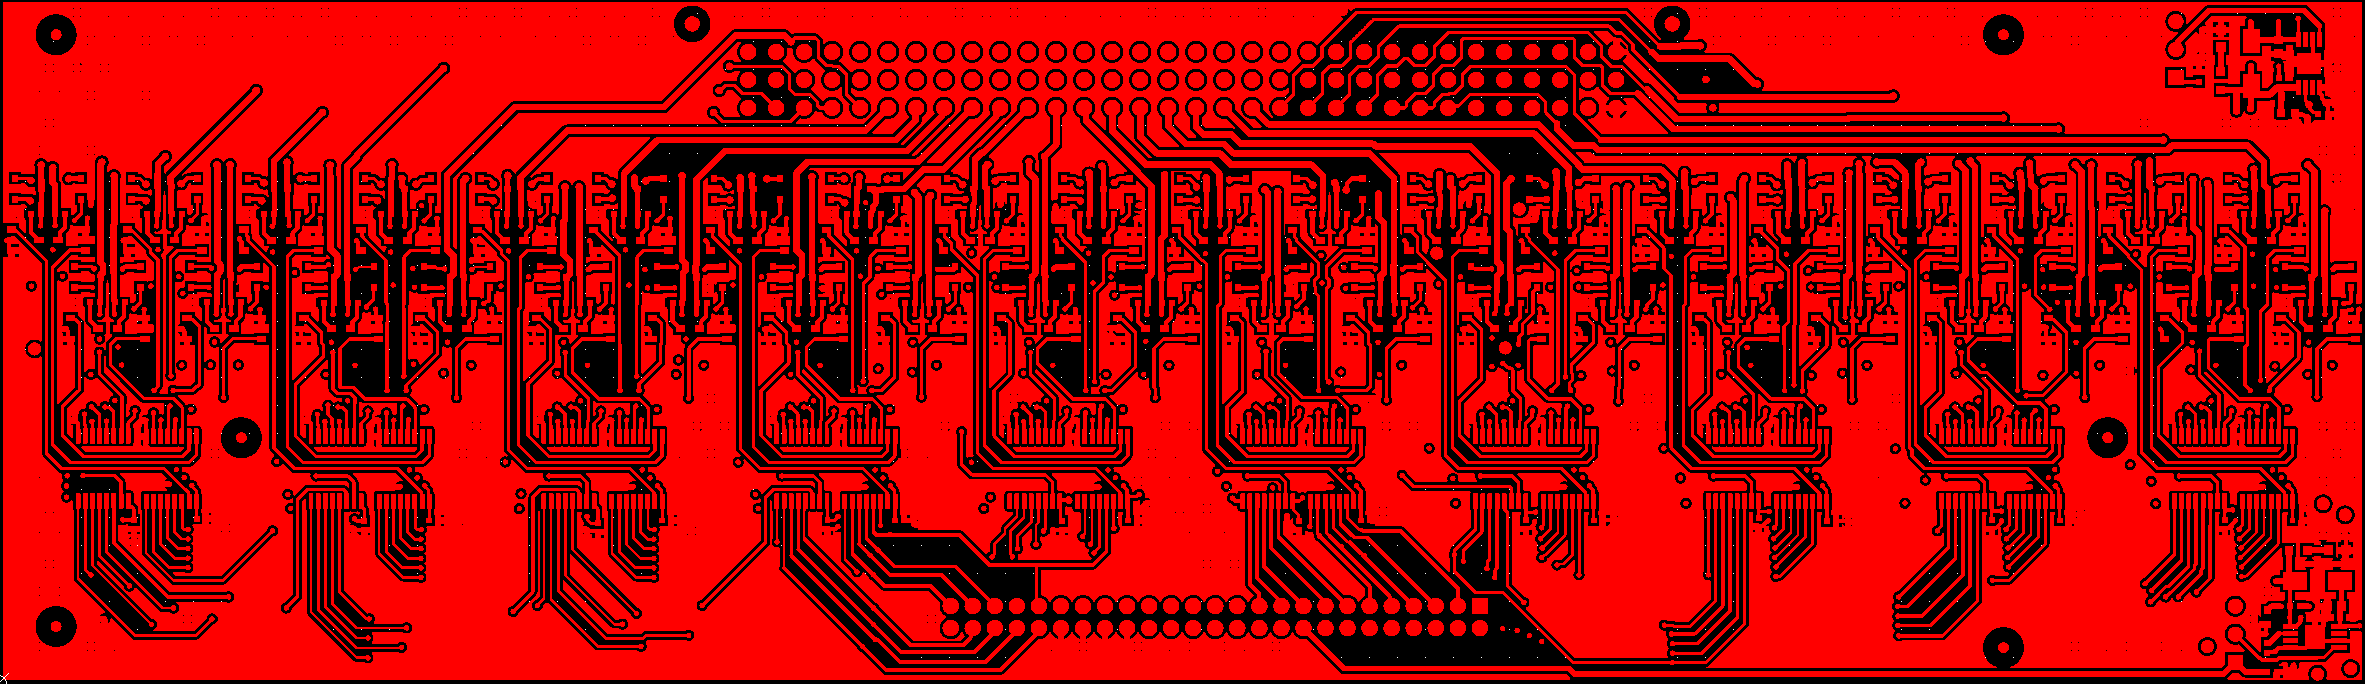
\includegraphics[height = 0.15\textheight]{obrazky/layer_top.png}
    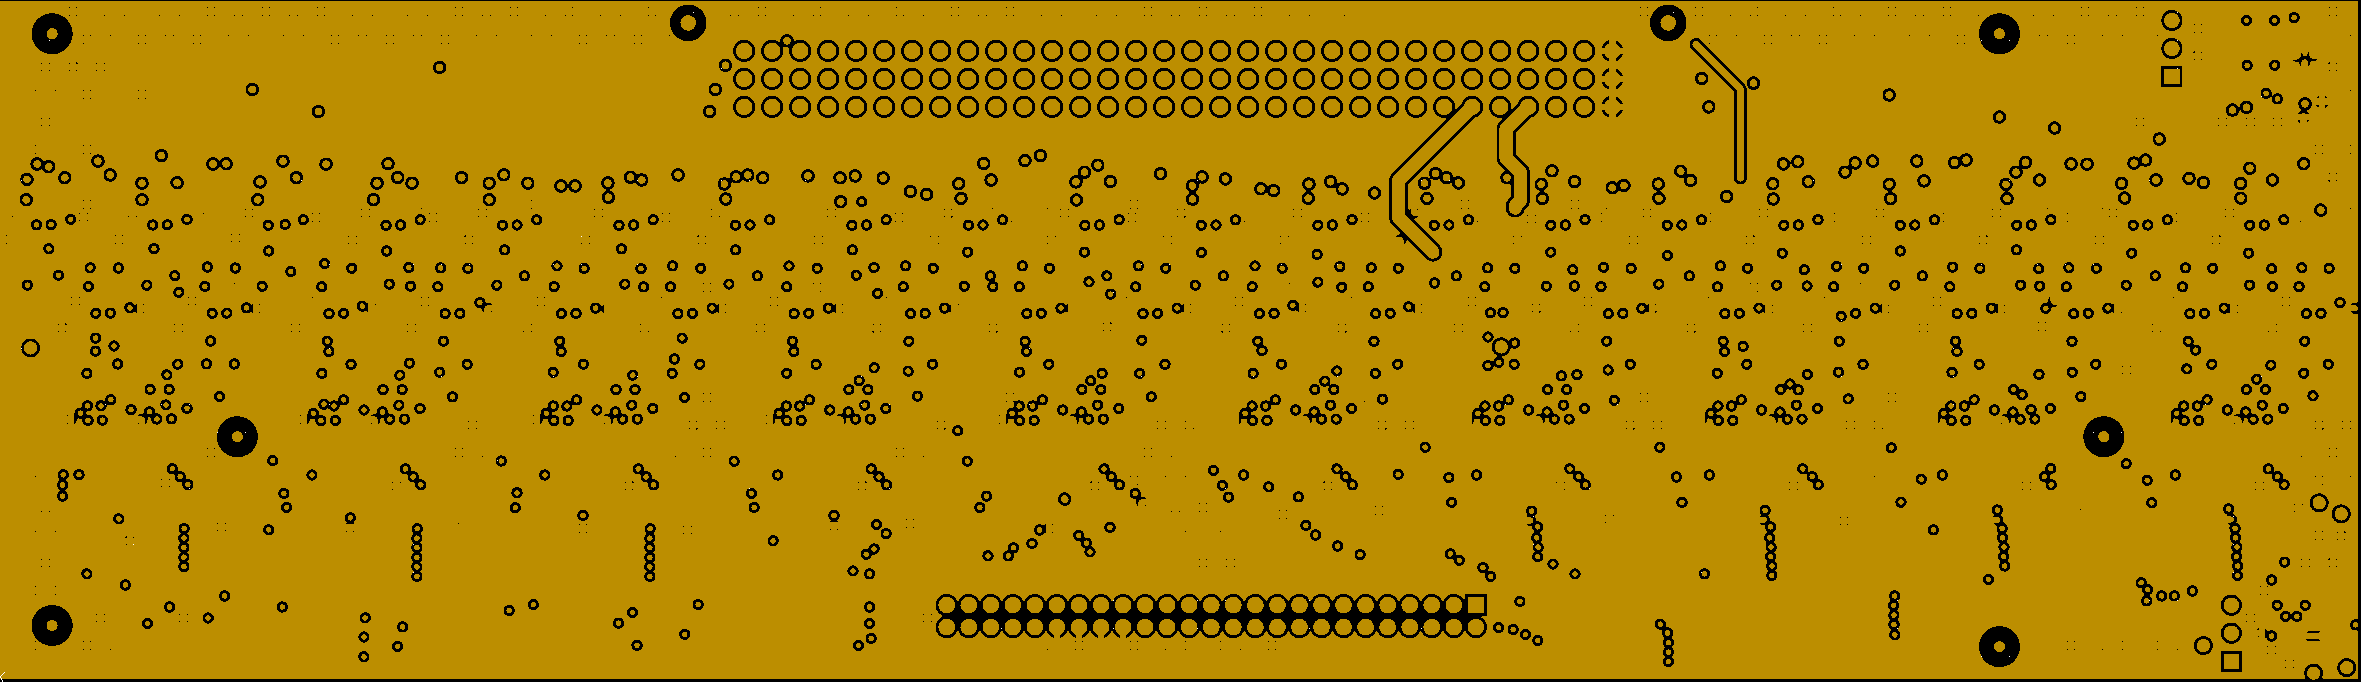
\includegraphics[height = 0.15\textheight]{obrazky/layer_2.png}
    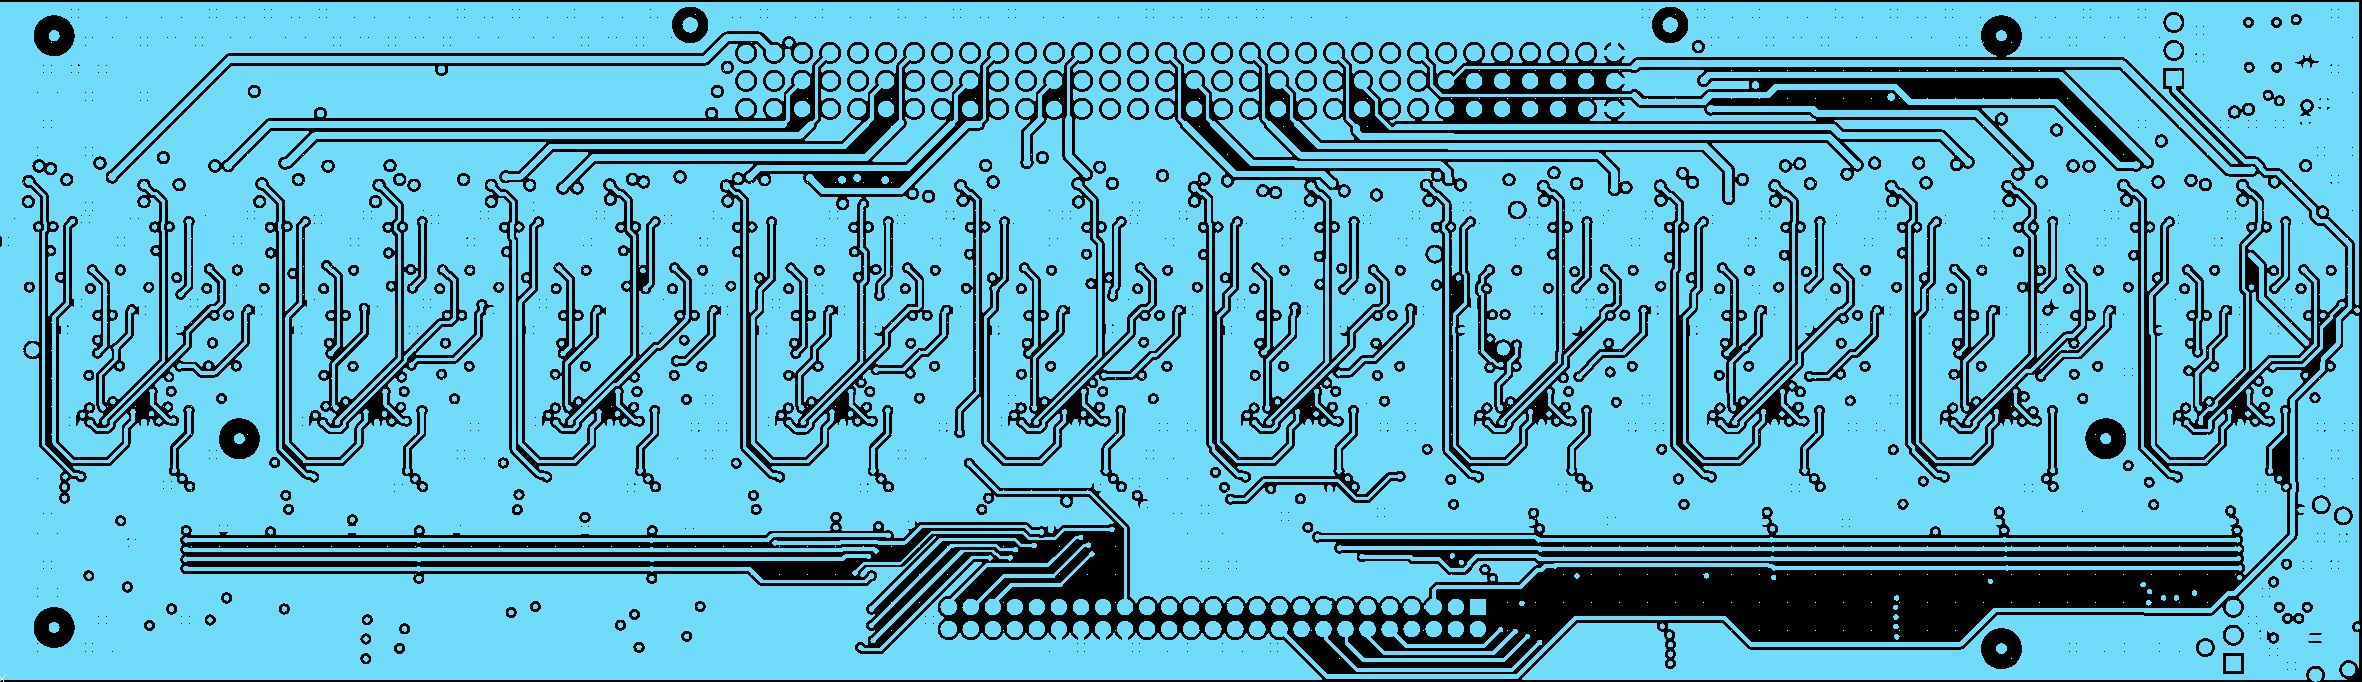
\includegraphics[height = 0.15\textheight]{obrazky/layer_3.png}
    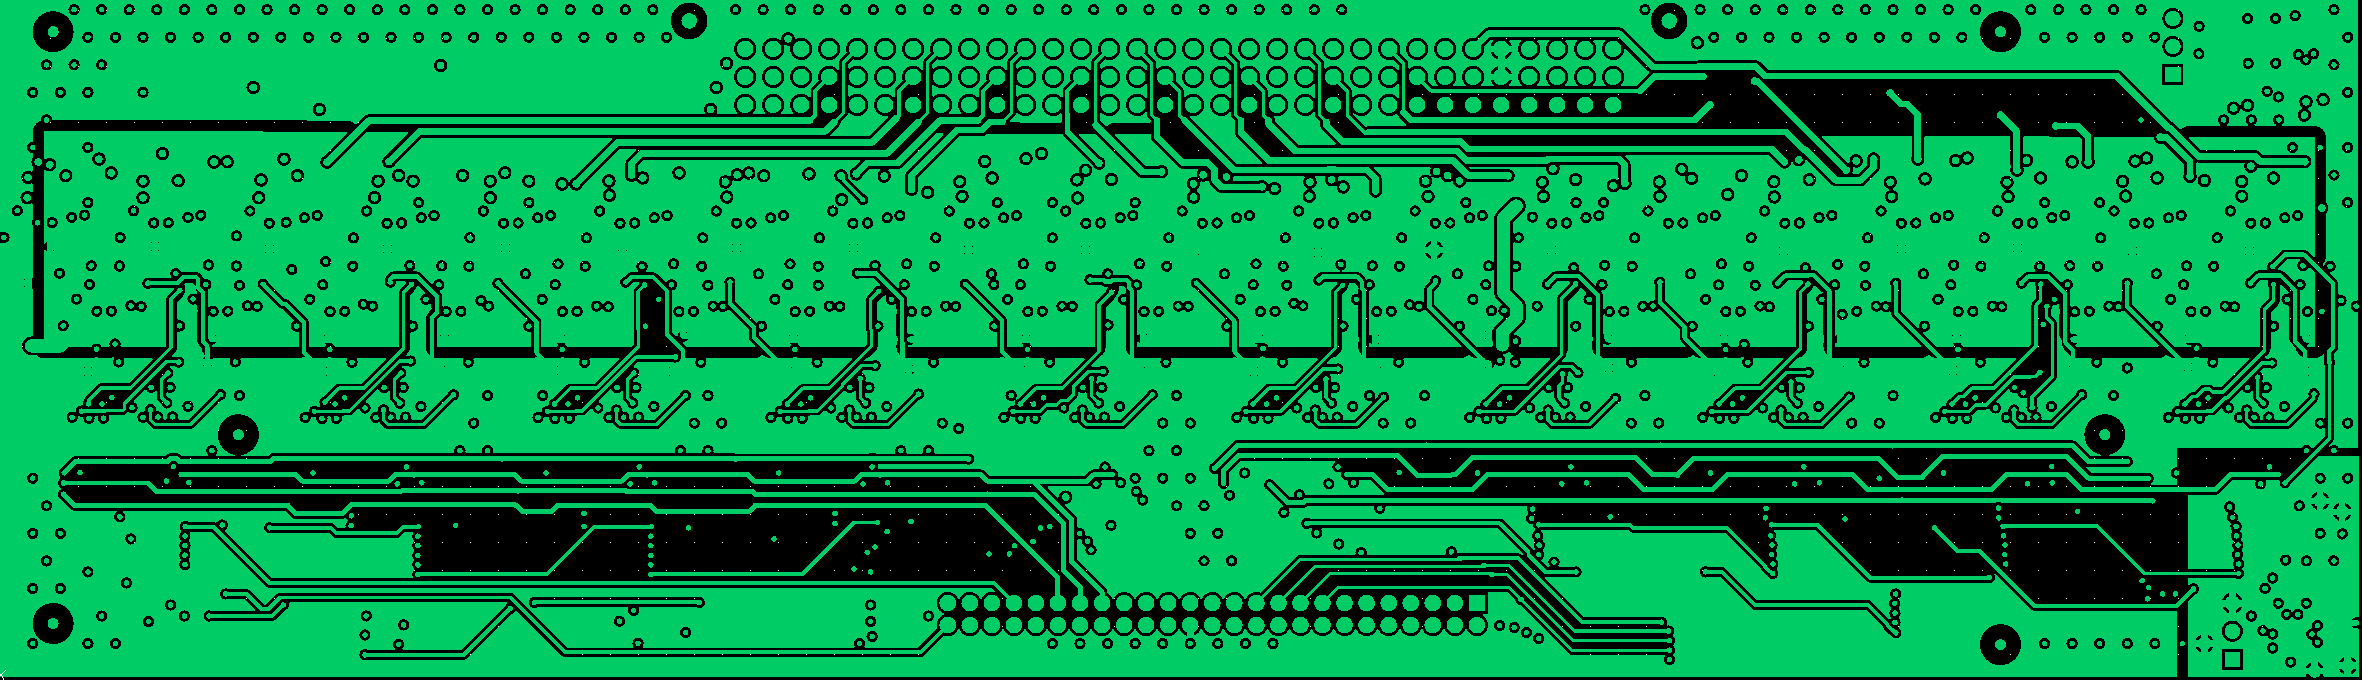
\includegraphics[height = 0.15\textheight]{obrazky/layer_4.png}
    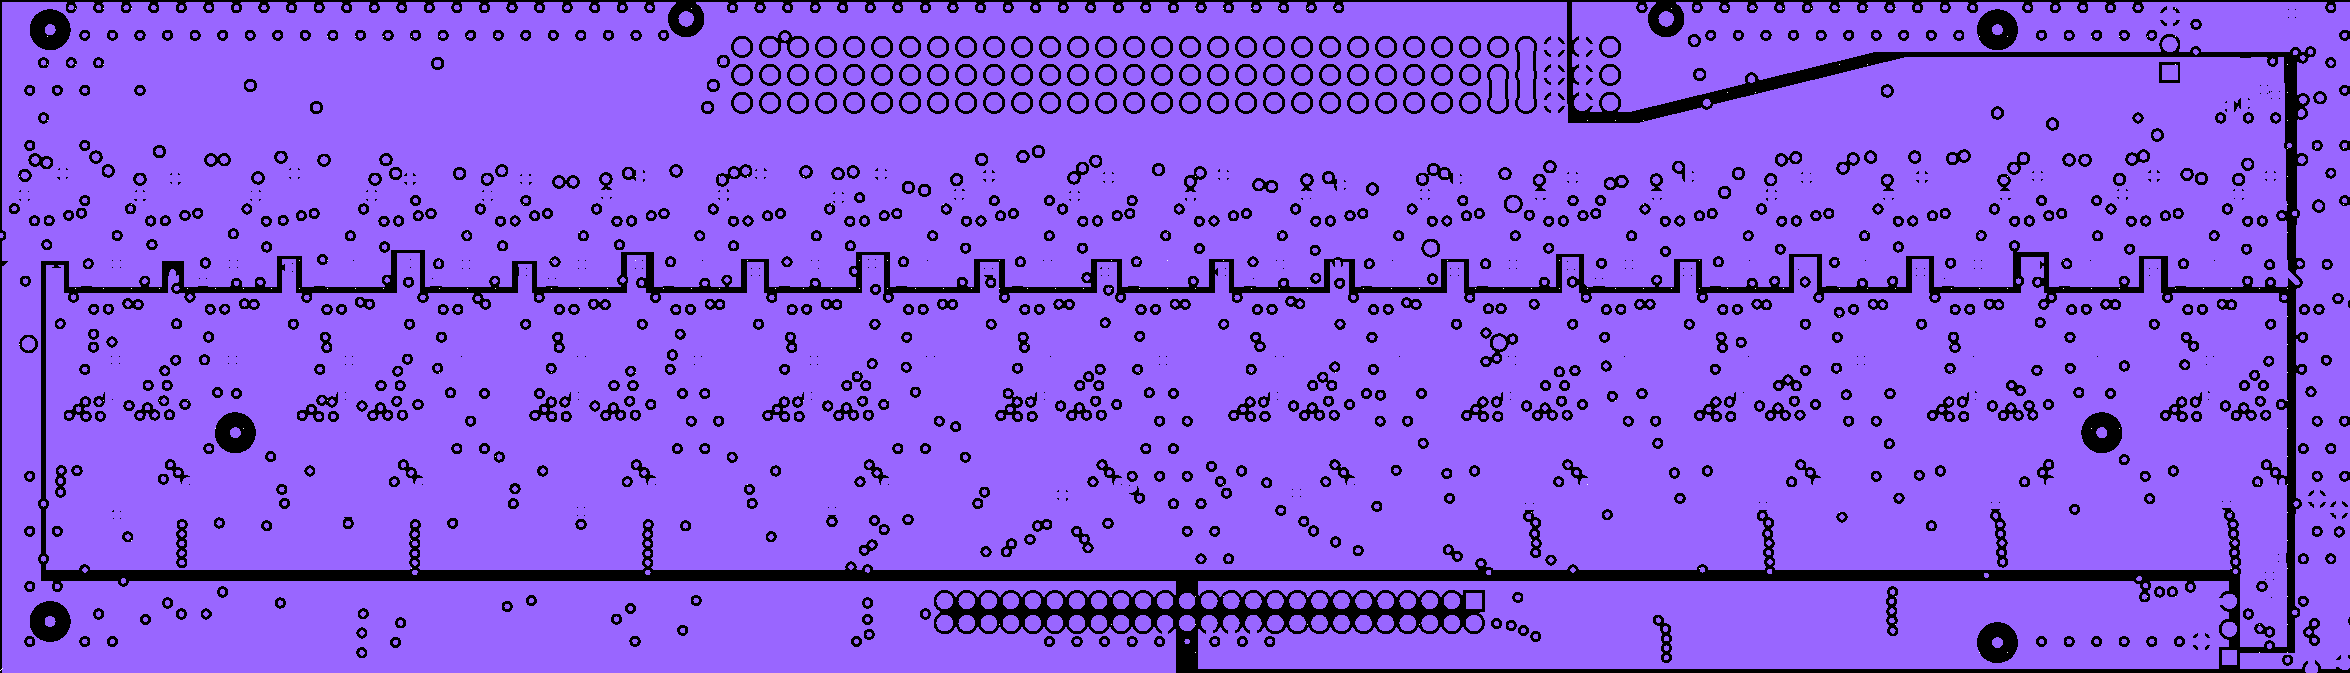
\includegraphics[height = 0.15\textheight]{obrazky/layer_5.png}
    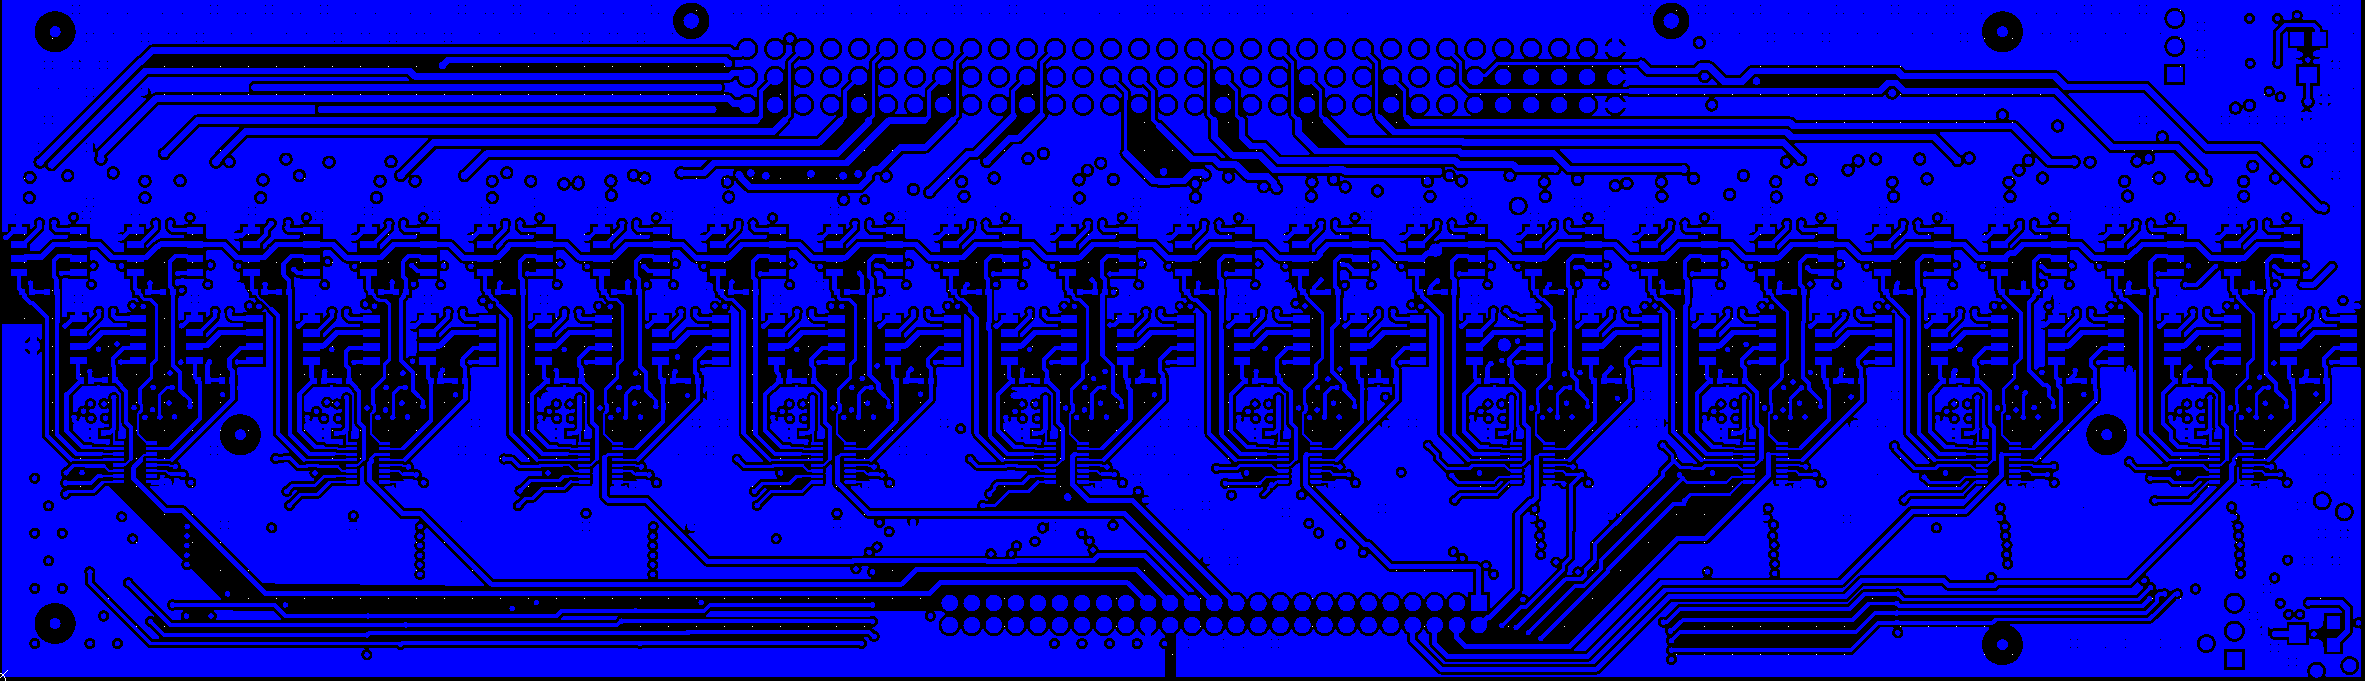
\includegraphics[height = 0.15\textheight]{obrazky/layer_bot.png}
    \caption{Vrstvy PCB top to bottom včetně polygonů}
    \label{fig:Vrstvy PCB top to bottom}
    
\end{figure}

\clearpage

Pro minimalizaci zemních smyček jsou po celé desce rozmístěny stitching vias,
které propojují GND signály.
V gerber datech a 3D modelu jsou stitching vias zobrazeny jako tented vias. Nicméně kvůli nižší ceně výroby PCB
jsou použity odkryté vias.
Z důvodu požadavků na osazení komponent byl použita použita ENIG povrchová úprava.\\

Důležitou podmínkou návrh PCB měřících karet je, že jejich výška (včetně komponentů) nesmí přesáhnout 8mm.
Tento rozměr je dán roztečí jednotlivých řad bRC pinů. Na následujících obrazcích jsou zobrazeny 3D modely měřící karty
s DIN konektorem, který přesahuje výšku 8mm (nebude však osazen). Finální rozměry měřící karty bez DIN konektoru jsou
(délka x šířka x výška) 215 x 62.5x 7.65mm. PCB obsahuje několik děr pro uchycení pomocí M3 šroubů.


\begin{figure}[ht!]
    \centering
    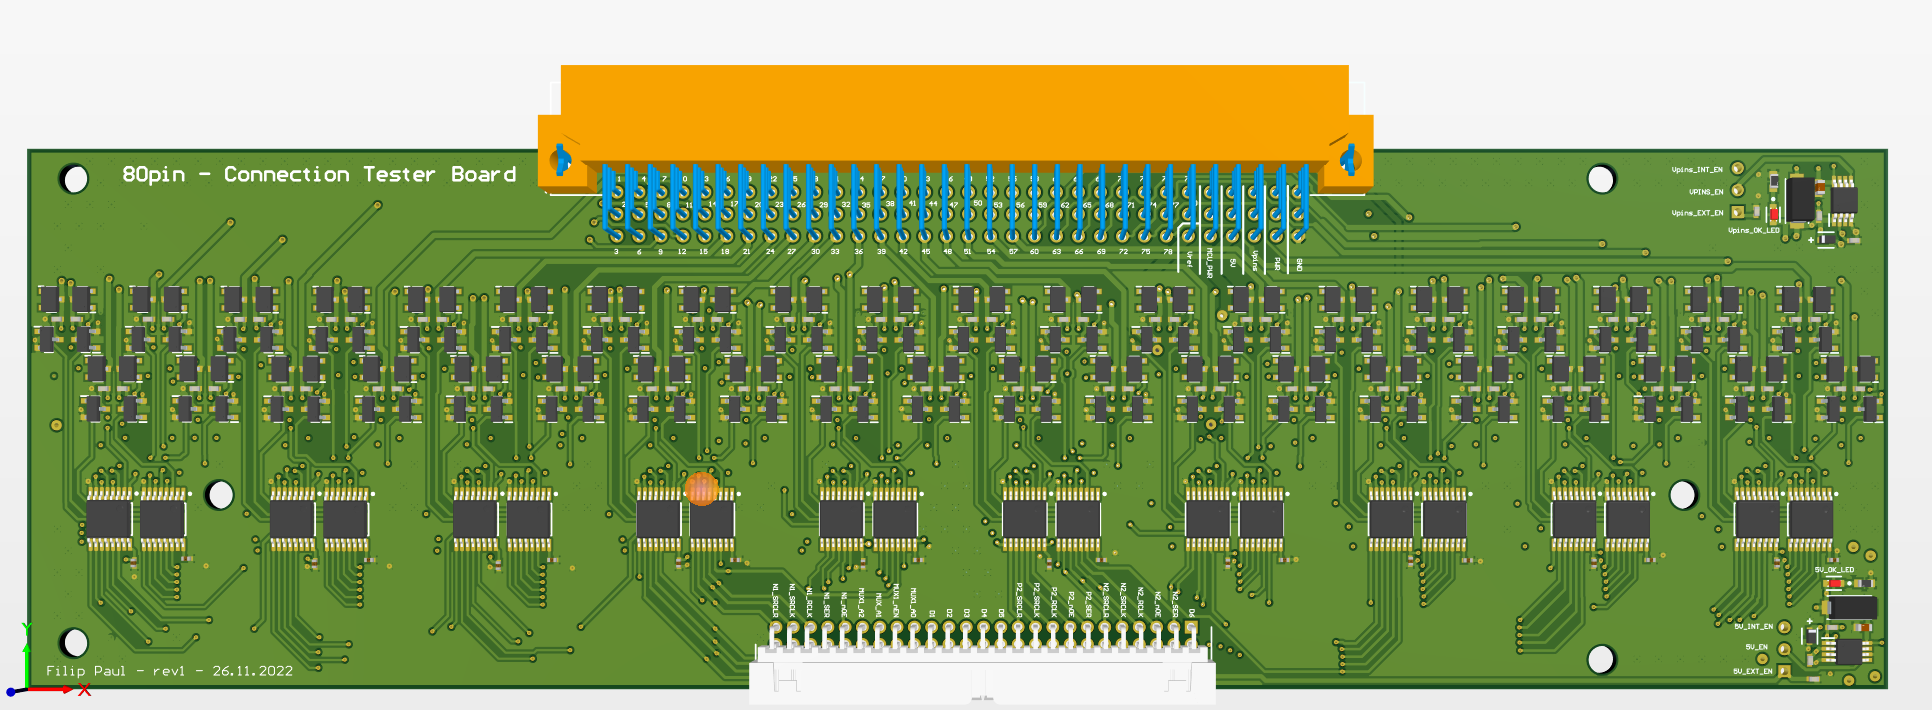
\includegraphics[width = 1\textwidth]{obrazky/karta_3D.png}
    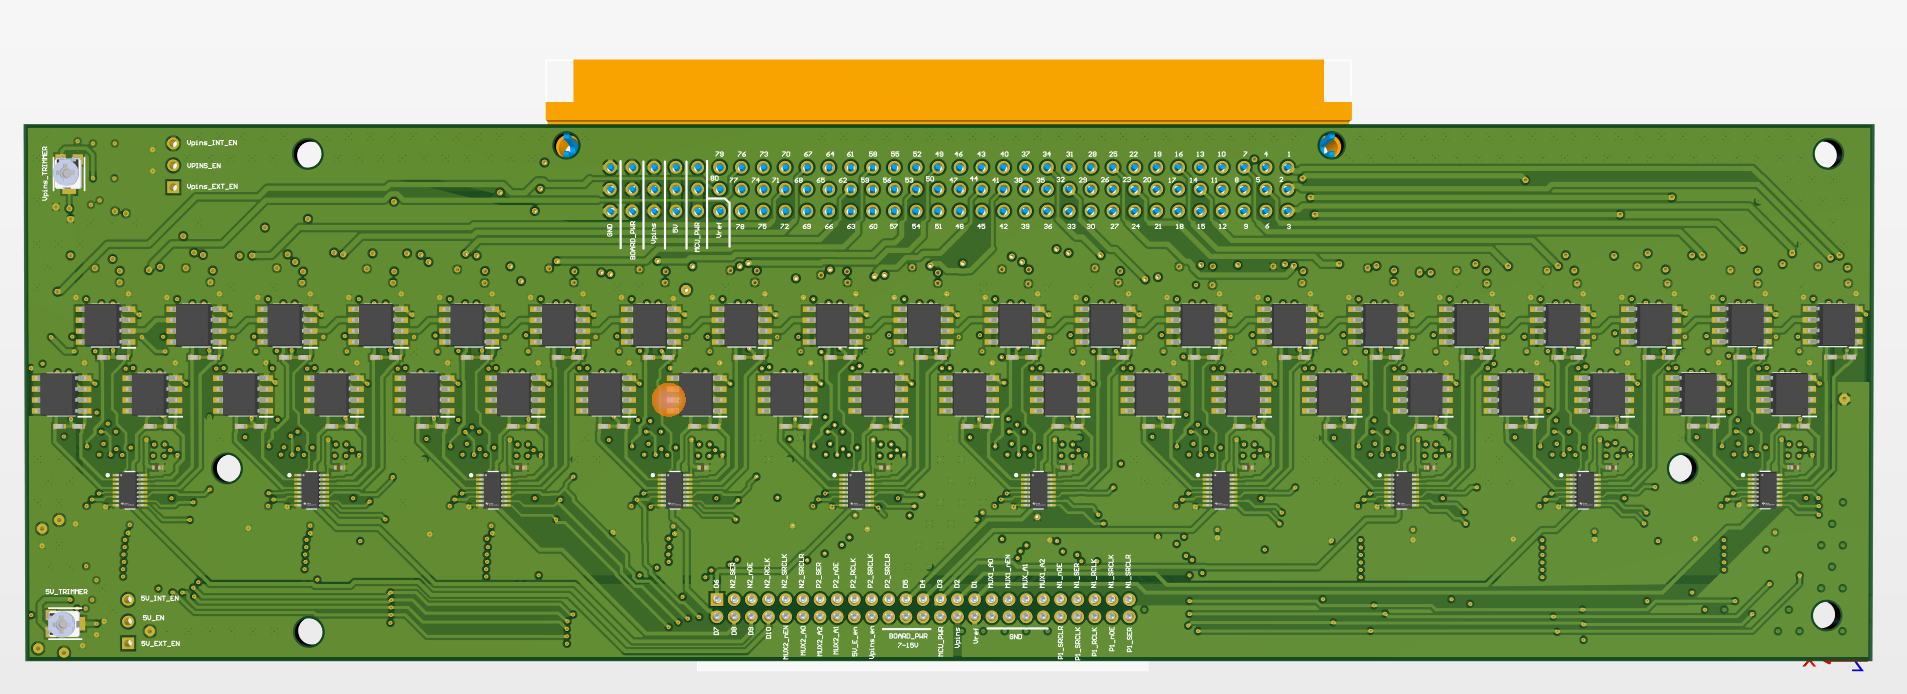
\includegraphics[width = 1\textwidth]{obrazky/karta_3D_bot.png}
    \caption{3D model top a bot s osazeným DIN konektorem}
    \label{fig:3D model top a bot}
    
\end{figure}




\chapter{Návrh ovládacích karet}
\section{Základní požadavky na Ovládací karty}
    Následující seznam popisuje základní požadavky na ovládací karty, seznam je seřazen podle priorit.
    \begin{enumerate}
        \item Schopnost ovládat měřící karty.
        \item Možnost komunikace pomocí 100\,Mbit Ethernetu.
        \item Dostupnost komponentů.
        \item Cena komponentů.
    \end{enumerate}

    \section{Funkční bloky}
    \begin{figure}[ht!]
        \centering
        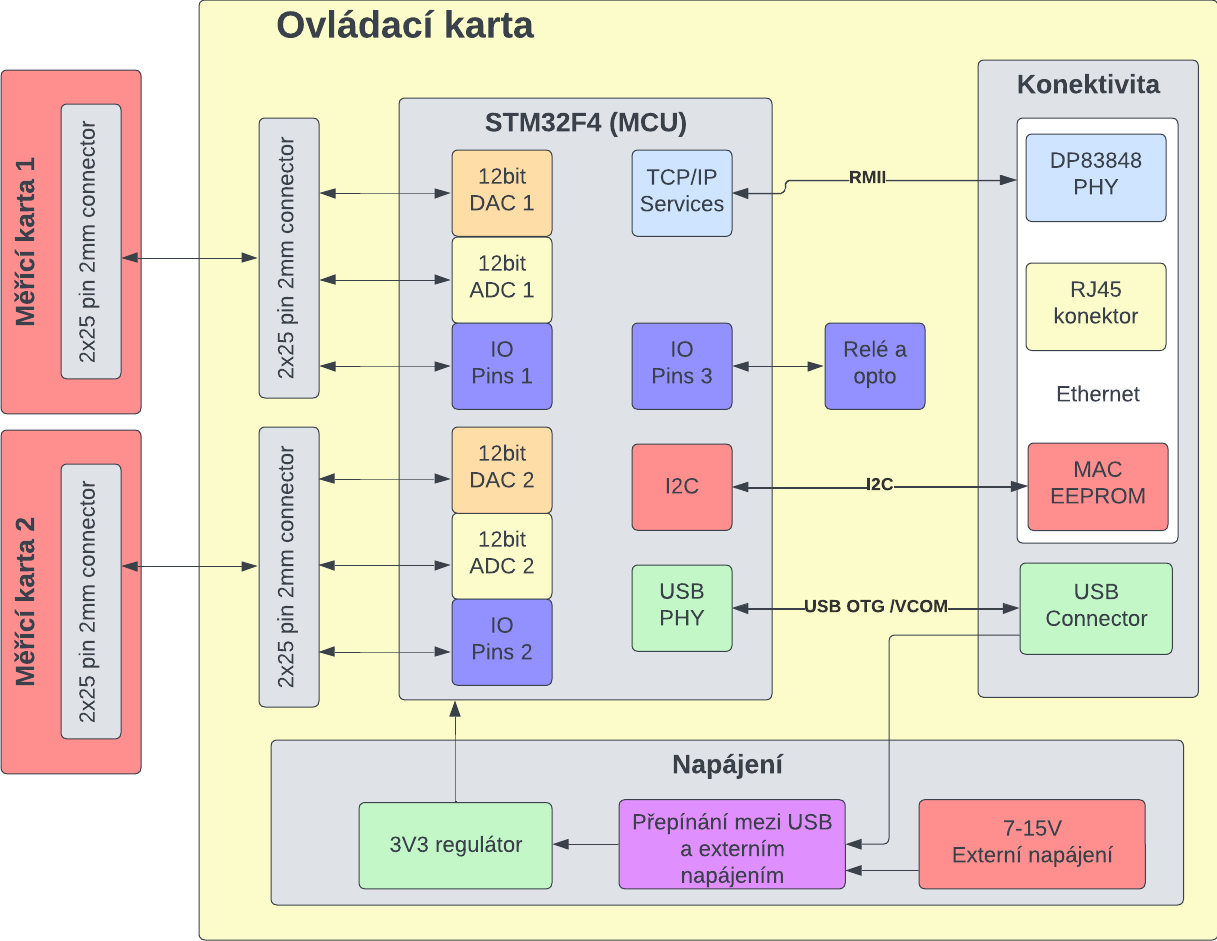
\includegraphics[width = 1\textwidth]{obrazky/ovladaci_karta_diag.png}
        \caption{Funkční diagram ovládací karty}
        \label{fig:Funkční diagram ovládací karty}
        
    \end{figure}

    Ovládací karta obsahuje několik pomyslných funkčních bloků (Obr. \ref{fig:Funkční diagram ovládací karty}).
    Jednotlivé bloky jsou podrobněji popsány v následujících kapitolách. Celé schéma k ovládací kartě je v příloze
    na konci tohoto dokumentu.

    \subsection{Mikrokontrolér a jeho periférie}
    Ovládací karta je založena na 32-bitovém mikrokontroléru STM32F407ZGT6 s Cortex M4 jádrem.
    Tento mikrokontrolér disponuje 114 I/O piny (3V3 logika), dvěma nezávislými 12-bit A/D a D/A převodníky,
    nativní podporou USB OTG a 100\,Mbit Ethernet MAC vrstvou. Právě díky těmto vlastnostem, je tento
    mikrokontrolér vhodný pro ovládání měřících karet a komunikaci s PC.\\

    Pro komunikaci s PC aplikací se primárně počítá s telnet serverem,
    který běží na mikrokontroléru. Nicméně pro debugovací
    účely je možno s ovládací kartou komunikovat i pomocí USB.
    K programování mikrokontroléru lze použít interface SWD, JTAG nebo DFU (USB bootloader).\\

    Jednotlivé shift registry a multiplexery jsou ovládány, skrze ovládací kartu, pomocí metody bit bangingu.
    Dále ovládací karta poskytuje 12-bitový DA a AD převodník.\cite{MARTINT}.\\

    Ovládací karta obsahuje i další periferie jako například CAN, LIN, RTC, opticky oddělené vstupy a výstupy apod.
    Tyto periferie slouží k použití karty v jiném projektu než je právě diplomová práce a proto nejsou podrobněji diskutovány.


    \subsubsection{D/A převodník}
    STM32F407ZGT6 nabízí dva 12-bit D/A převodníky s možností využití integrovaného bufferu v podobě
    invertujícího operačního zesilovače. Nicméně podle datasheetu
    je možné použít výstupní buffer pouze do velikosti kapacitní zátěže 50\,pF.
    Kapacitní zátěž D/A převodníku bude rovna parazitním kapacitám, které nelze jednoznačně určit
    a vstupní kapacitě 80 komparátorů (V+ proti GND). Každý z komparátorů má svou vstupní kapacitu
    přibližně 3\,pF. Dohromady tedy vznikne kapacitní zátěž minimálně 240\,pF.\cite{DAC}\\
    \begin{figure}[ht!]
        \centering
        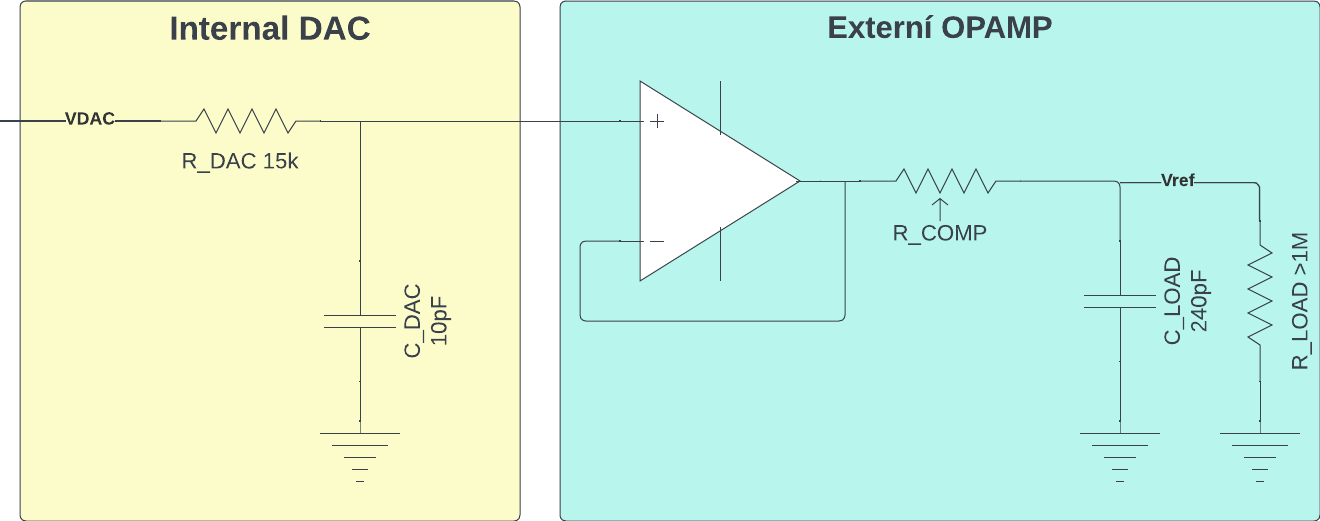
\includegraphics[width = 1\textwidth]{obrazky/DAC_OPAMP.png}
        \caption{DAC-externí zesilovač}
        \label{fig: DAC-externí zesilovač}
        
    \end{figure}

    Pro použití D/A převodníku je použit externí operační zesilovač v zapojení (Obr. \ref{fig: DAC-externí zesilovač}).
    V tomto zapojení je rychlost D/A převodníku limitována kapacitou pinu D/A převodníku C\_DAC (cca 10\,pF)
    a vnitřním odporem R\_DAC (cca 15\,k$\Omega$). Mezní kmitočet nezatíženého D/A převodníku pak lze určit následovně.
    \begin{equation}
        f_{max} = \frac{1}{2\pi \cdot  C_{dac} \cdot  R_{dac}} = \frac{1}{2\pi \cdot 10\,pF \cdot 15\,k\Omega} = 1,06\,MHz
    \end{equation}

    Kapacitní zátěž společně s výstupním odporem operačního zesilovače by mohla
    způsobit nestabilitu a s tím spojené nežádoucí oscilace v časové oblasti.
    Z tohoto důvodu datasheet použitého operačního zesilovače AD8531 doporučuje použít v případě vyšší kapacitní zátěže tzv. snubber network.
    V datasheetu je možno nalézt následující hodnoty součástek pro různou kapacitní zátěž (v Obr. \ref{fig: DAC-externí zesilovač} realizováno
    kombinací součástek C\_SNUBB a R\_COMP).
    \begin{figure}[ht!]
        \centering
        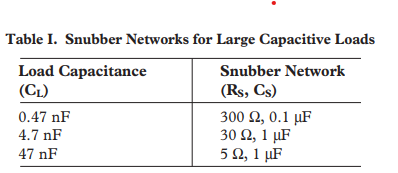
\includegraphics[]{obrazky/snubber_values.png}
        \caption{Snubber Network (obrázek převzat z \cite{OPA_datasheet})}
        \label{fig: Snubber Network}
    \end{figure}

    Protože datasheet neuvádí hodnoty součástek pro kapacitní zátěž 240\,pF, je odpor R\_COMP realizován
    trimmerem pro možnost kalibrace. Hodnota kapacity C\_SNUBB byla zvolena 100\,nF.\\
    Kalibrace je prováděna tak, že se na výstupu D/A převodníku nastaví obdélníkový
    signál o frekvenci 500\,kHz a poté se trimmerem nastaví taková hodnota, aby v časové oblasti
    byl co nejmenší překmit\cite{DAC_stability,OPA_stability}.\\

    \subsubsection{Programování a debuging}
    Pro účely debugování a programování mikrokontroléru jsou zpřístupněny SWD a JTAG piny.
    Dále je možno modifikovat konfiguraci mikrokontroléru pomocí jumperů, které jsou propojeny
    s boot piny mikrokontroléru. Při normálním provozu se počítá s programováním pomocí SWD rozhraní.
    Případně je také možné mikrokontrolér naprogramovat přes USB konektor pomocí zabudovaného DFU.

    \subsubsection{Konfigurace hodinového signálu}
    
    Mikrokontrolér má vysokou variabilitu v konfiguraci hodinových signálů.
    K požadovaným funkcím ovládací karty je vhodné použít externí krystalový rezonátor, který bude
    připojen do High Speed Clock pinů mikrokontroléru. V případě ovládací karty bylo použit 8\,MHz
    krystalového rezonátoru ABM3B-8.000MHZ-D2-T společně s 2x27\,pF zatěžovacími kapacitory.\\

    %%\begin{figure}[ht!]
    %%    \centering
    %%    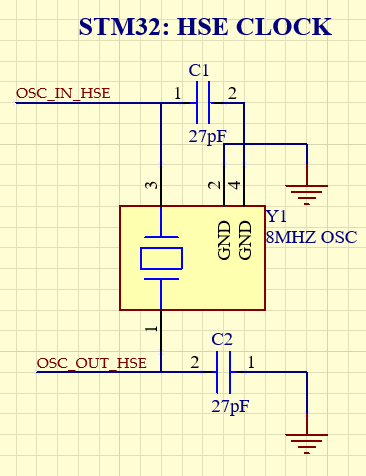
\includegraphics[height = 0.2\textheight]{obrazky/CLK_rezonator.png}
    %%    \caption{8\,MHz krystalový rezonátor}
    %%    \label{fig: MHz krystalový rezonátor}
    %%\end{figure}

    Pro jednodušší konfiguraci hodinových signálů mikrokontroléru bylo využito programu STM32CubeMX.
    Výsledná konfigurace hodinových signálů je znázorněna na následujícím obrázku.

    \begin{figure}[ht!]
        \centering
        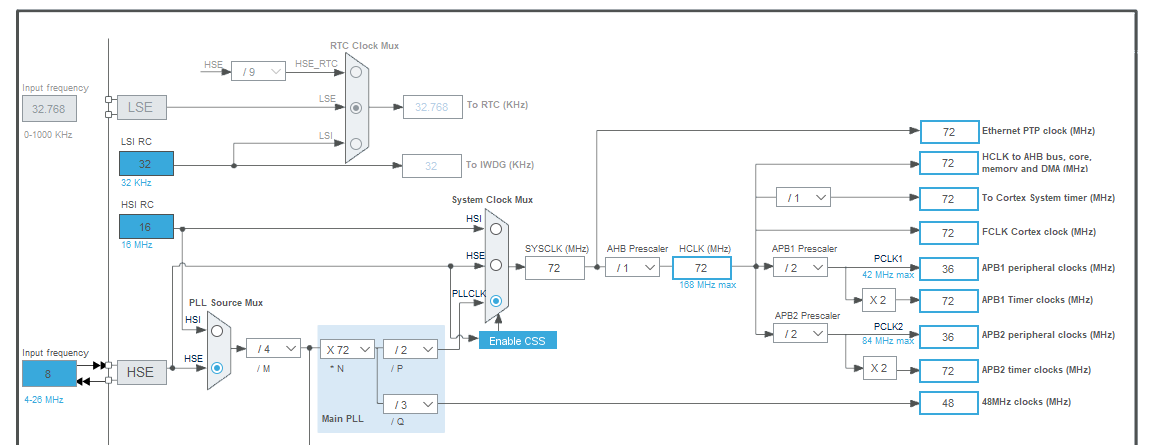
\includegraphics[width = 1\textwidth]{obrazky/CLK_config.png}
        \caption{Clock configuration}
        \label{fig: Clock configuration}
    \end{figure}

    \subsection{Konektivita}
    Ovládací karta je vybavena USB-micro a RJ45 konektorem. Umožňuje tak velmi snadné propojení s PC aplikací
    pomocí standardních USB a ethernetových rozhraní.

    \subsubsection{Ethernet}
    Pro zajištění ethernetového připojení je využito MAC
    vrstvy mikrokontroléru společně s fyzickou vrstvou (PHY)
    realizovanou pomocí čipu DP83848 a RJ45 konektoru s integrovaným transformátorem pro 100 BASE-T. Komunikace mezi
    mikrokontrolérem a DP83848 je realizováno pomocí RMII rozhraní. PHY vyžaduje pro svou správnou funkčnost
    100$\Omega$ diferenciální páry (viz. schéma ovládací karty v příloze).\\
    
    DP83848 vyžaduje pro svou činnost v RMII režimu připojení externího 50\,MHz oscilátoru.
    Výstup oscilátoru je zároveň přiveden na příslušný pin mikrokontroléru a slouží jako 
    hodinová reference.\\ 

    DP83848 je možno konfigurovat pomocí tzv. bootstrap pinů. DP83848 při svém startu zjišťuje
    logické úrovně bootstrap pinů a podle toho konfiguruje své parametry. Následující tabulka
    shrnuje nastavení bootstrap pinů použitých v ovládací kartě.

    \begin{table}[ht!]
        \resizebox{\columnwidth}{!}{%
        \begin{tabular}{|c|c|l|}
        \hline
        \textbf{PIN} & \textbf{Nastavení} & \textbf{Popis}                                   \\ \hline
        AN0 & 1 & AN0 a AN1 piny konfigurují, jakými možnostmi se bude zařízení prezentovat   při AutoNegotioation.   \\ \hline
        AN1 & 1 & Pro kombinaci AN0 = 1 a AN1 = 1 zařízení se prezentuje jako  10BASE-T a 100BASE-TX HALF/FULL duplex \\ \hline
        LED\_CFG     & 1                  & Konfiguruje chování LED na RJ45 konektoru.       \\ \hline
        MII\_MODE    & 1                  & DP83848 očekává RMII pro komunikaci s MAC vrstvou \\ \hline
        MDIX ENABLE  & 1                  & Interní pull up - MDIX (crossover) povolen       \\ \hline
        \end{tabular}%
        }
        \caption{Nastavení bootstrap pinů DP83848}
        \label{RMII settings}
        \end{table}


    Protože ani mikrokontrolér a ani DP83848 nenabízí jedinečnou MAC adresu je použita EEPROM,
    která má již od výrobce naprogramovanou jedinečnou MAC adresu.
    EEPROM používá ke komunikaci I2C protokol a při startu zařízení je MAC adresa
    načtena do MAC vrstvy mikrokontroléru. V mikrokontroléru je implementován telnet
    a http server a je využito LWIP stacku společně s HAL knihovnami a RTOS.\\

    \subsubsection{USB}
    Mikrokontrolér je vybaven fyzickou vrstvou pro USB OTG,
    je tak možné propojit datové signály přímo s USB-micro konektorem.
    Přestože je do USB konektoru vyveden ID pin, který slouží
    k rozlišení mezi host a device, využívá ovládací karta pouze device režim.
    Pro detekci připojení ovládací karty k USB portu je použit napěťový dělič, jehož výstup
    je přiveden do USB\_sense pinu mikrokontroléru. Napěťový dělič obsahuje rezistor o toleranci
    1\,\%. Tuto toleranci není nutno dodržet a tento rezistor byl použit pouze z důvodu nízké ceny
    a faktu, že se již v návrhu vyskytuje.\\

    Připojení pomocí USB slouží převážně k servisním účelům.
    Ovládací kartu lze napájet přímo z USB portu, přičemž napájení je opatřeno
    vstupním filtrem realizovaným feritovou perličkou a kondenzátorem (více v sekci o napájení).
    Obdobně jako u ethernetu je i zde nutno při návrhu PCB použít diferenciální páry
    pro datové signály (90\,$\Omega$). Každý ze signálů,
    který je vyveden na USB-micro konektor je opatřen TVS diodami pro ochranu
    proti ESD. \\

    \begin{figure}[ht!]
        \centering
        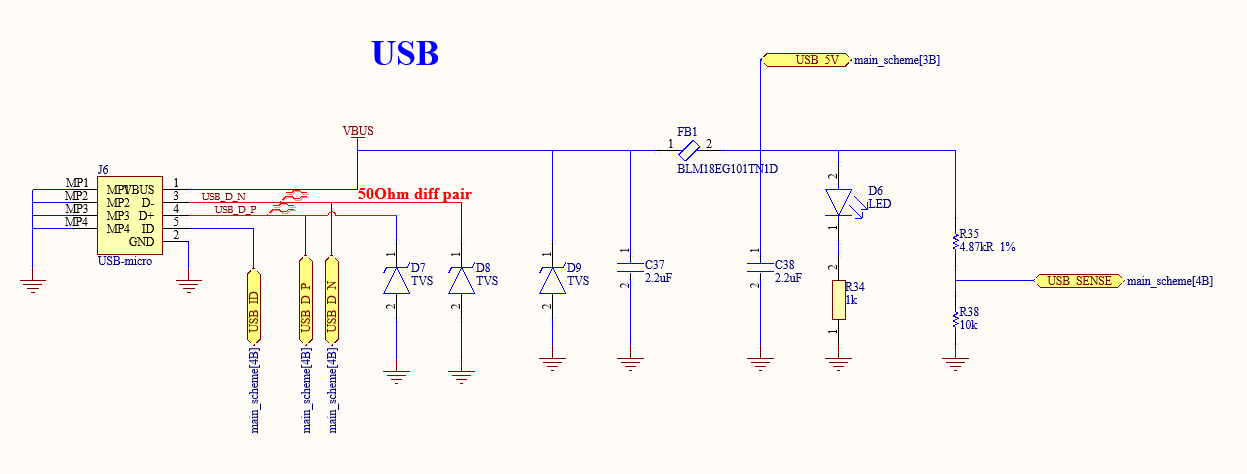
\includegraphics[width = 1\textwidth]{obrazky/USB.png}
        \caption{USB rozhraní}
        \label{fig: USB rozhraní}
    \end{figure}

\clearpage
    \subsection{Napájení}
    Při normálním provozu se počítá s externím napájení v rozmezí 7-15 VDC.
    Toto napětí je přivedeno na WAGO svorky. Napětí (ve schématu BOARD\_PWR)
    přivedeno na vstup nastavitelného regulátoru TLV76701DGNR. Funkce tohoto regulátoru je obdobná
    jako u regulátorů popsaných v sekci o měřící kartě. Výstup regulátoru je možné
    nastavit trimmerem v rozmezí přibližně od 2.8 do 3.45V (ve schématu 3v3\_MCUs).\\

    \begin{figure}[ht!]
        \centering
        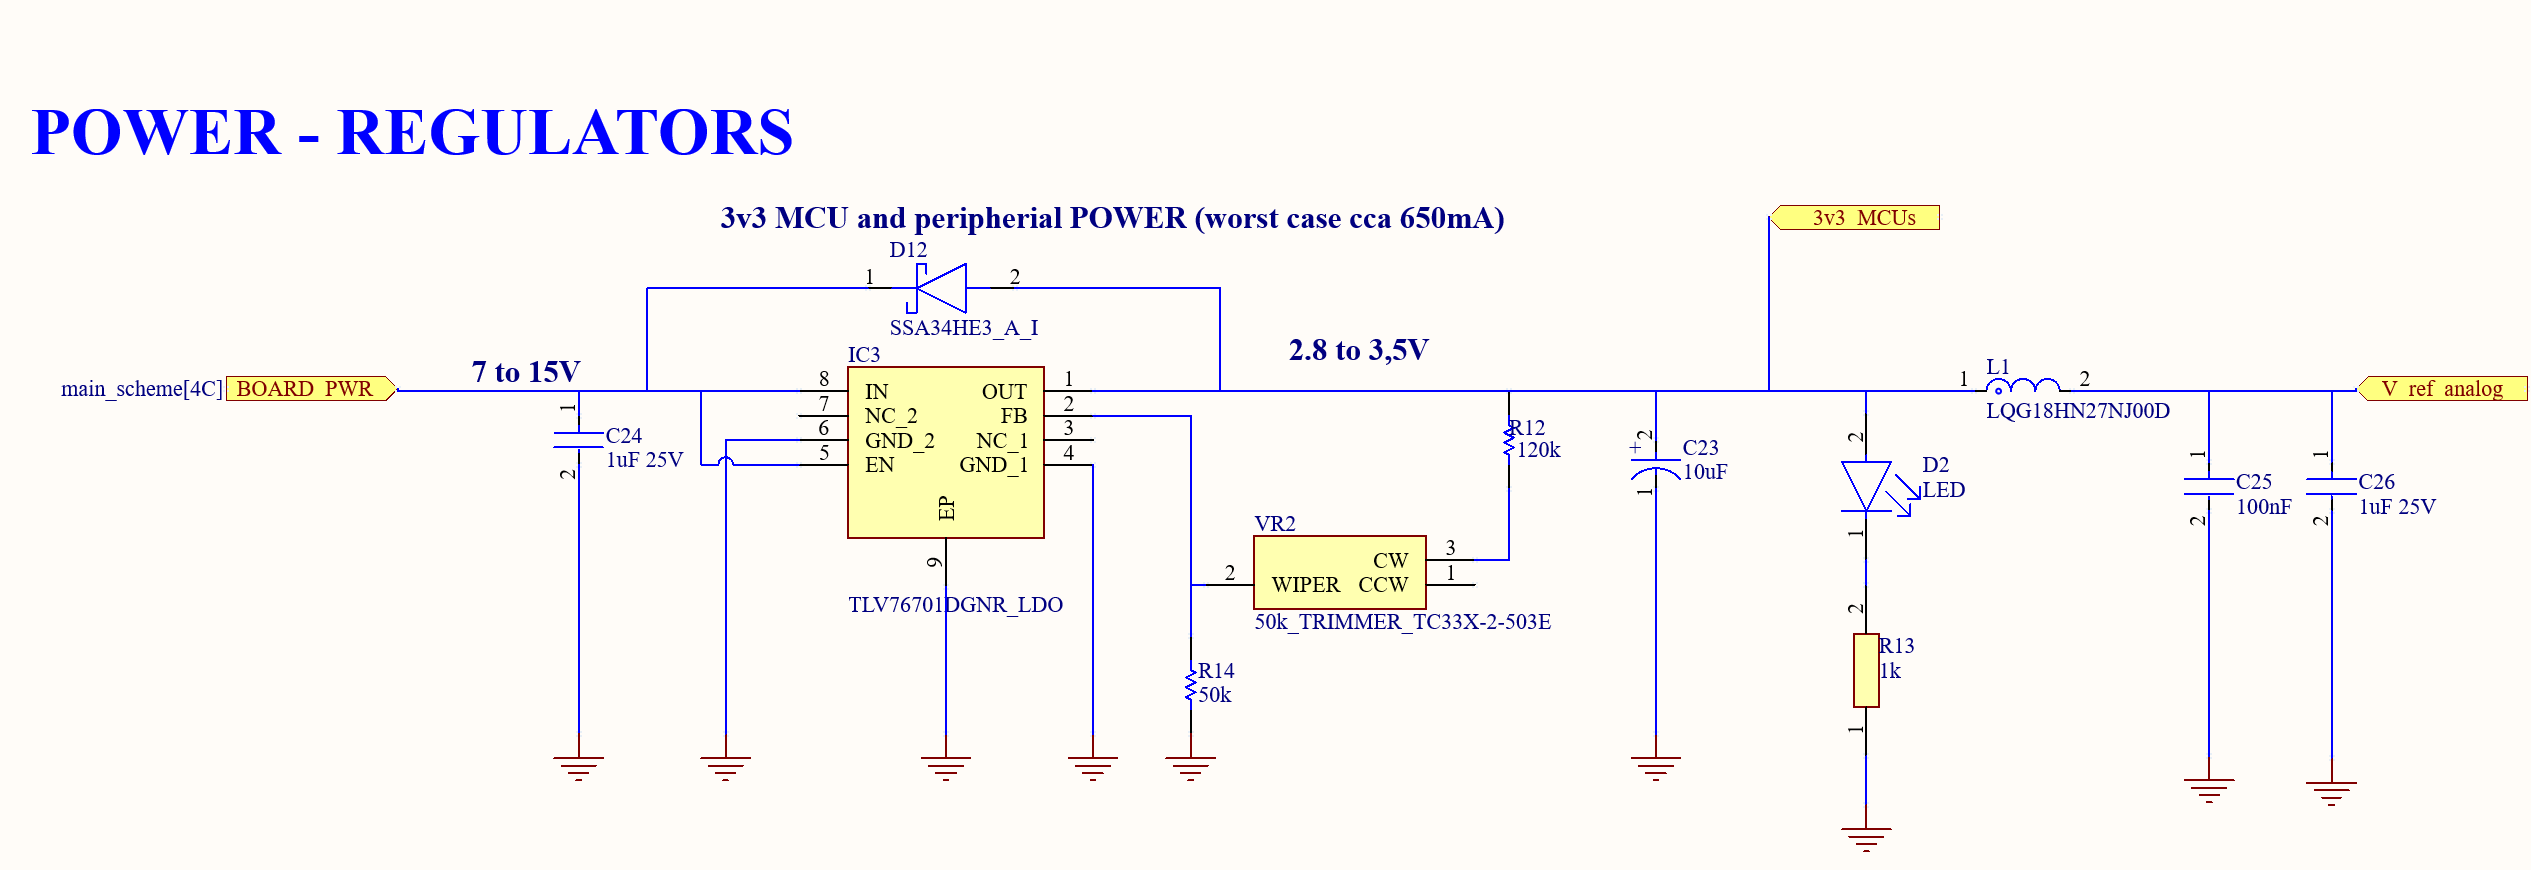
\includegraphics[width = 1\textwidth]{obrazky/PWR_REG_3V3.png}
        \caption{Regulátor napětí - 3V3 MCUs}
        \label{fig:Regulátor napětí - 3V3 MCUs}
    \end{figure}

    Takto regulované napětí je použito pro napájení všech doposud popsaných částí ovládací karty.
    Protože je vhodné aby referenční napětí (V\_ref\_analog),
    které mikrokontrolér používá  pro funkci A/D a D/A převodníků bylo co nejpřesnější, je
    napětí 3V3\_MCUs filtrováno dolní propustí realizovanou pomocí LC filtru.\\

    Očekávaný maximální proud fyzické vrstvy ethernetu je přibližně 150\,mA.
    Proudový odběr ovládací karty nelze jednoznačně určit,
    protože je závislý na firmwaru mikrokontroléru.
    Nicméně se očekává, že by proud v nejhorším případě neměl přesáhnout 500\,mA. 
    Použitý regulátor by měl být schopen dodat do obvodu proud 1A, což by
    mělo být dostačující.\\ 
    
    Napětí je dále přivedeno na 2x25 pinový konektor,
    aby bylo možné napájet měřící a ovládací karty současně připojením napájecí napětí pouze
    na jednu z karet.\\

    Celý systém měřících a ovládacích karet může být napájen pomocí USB. V tomto případě je však přesnost
    měření limitována kvalitou USB napájení. Následující obrázek znázorňuje distribuci napájení
    ovládacích a měřících karet. Schéma však neodpovídá reálnému zapojení, protože jednotlivé
    komponenty jsou propojeny přes 2x25 pin konektory. Pro přehlednost jsou však konektory vynechány.
    \clearpage


    \begin{figure}[ht!]
        \centering
        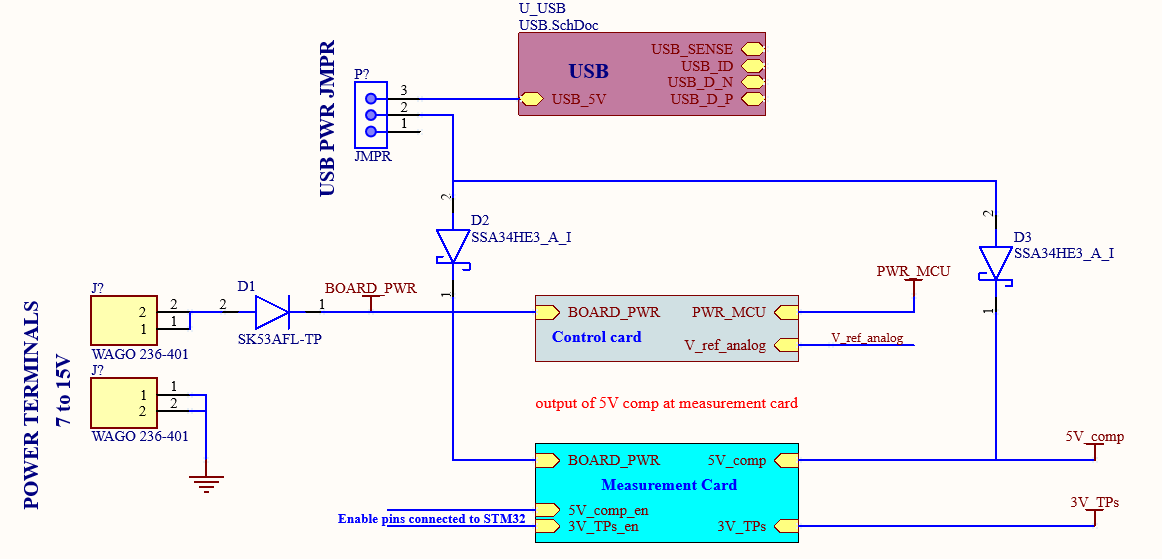
\includegraphics[width = 1\textwidth]{obrazky/USB_power_distr.png}
        \caption{Distribuce napájení}
        \label{fig:Distribuce napájení}
    \end{figure}

    V případě napájení pomocí USB je napětí BOARD\_PWR generováno z USB portu.
    Aby se zamezilo poškození všech připojených zařízení, které by mohlo potenciálně vzniknout připojením
    vyššího napětí na WAGO svorkách a USB současně, je do schématu připojena dioda D2. Dioda D1
    slouží jako ochrana k přepólování na vstupu WAGO svorek. Zároveň dioda D1 plní obdobnou funkci jako dioda D2
    nyní však pro ochranu zdroje napájení připojeného do WAGO svorek proti napětí na USB.
    V případě současného připojení externího napětí na WAGO svorky a USB portu, bude deska napájena
    vyšším z napětích.\\

    Napětí BOARD\_PWR je v případě napájení přes USB rovno přibližně:
    
    \begin{equation}
        V_{BOARD\_PWR} = V_{USB} - V_{D2} = 5V - 0.4V = 4.6V,
    \end{equation}
    Kde $V_{D2}$ je úbytek na diodě D2. Tento úbytek je pro diodu SSA34HE3\_A\_I roven přibližně 0.2V při proudu 1A
    a přibližně 0.4V při proudu 2A\\

    Úbytek napětí na regulátorech TLV76701DGNR je přibližně 0.8V.
    Součtem úbytků na diodě D2 a regulátoru lze 
    dosáhnou regulovaného výstupního napětí až 3.8V, což je dostatečné pro napájení všech regulátorů
    kromě regulátoru, který zajišťuje napětí 5V\_comp. Napětí 5V\_comp je tedy generováno přímo z USB portu přes 
    diodu D3. Dioda D3 má obdobný význam jako dioda D2, nyní však chrání USB port před vyšším napětím na výstupu
    regulátoru 5V\_comp v případě napájení z WAGO svorek. Z tohoto je patrné, že napětí 5V\_comp není nijak regulováno
    a je přímo závislé na napětí a rušení USB portu.
    V případě detekce napětí na USB\_sense pinu je komparátor 5V\_comp vypnut pomocí enable pinu.\\

    Pro možnost použití USB rozhraní pouze pro komunikaci (ne pro napájení),
    lze USB napájení rozpojit pomocí jumperu.\\


    \subsection{PCB -design}
   Stejně jako u návrhu měřící karty byl při návrhu ovládací karty použit software ALTIUM Designer.
   PCB je 6-ti vrstvé s řízenými impedancemi pro diferenciální páry USB a Ethernet fyzických vrstev.
   Pro určité cesty je zajištěna stejná délka cest pro správnou funkčnost rychlých signálů.
   Podrobnější informace lze nalézt v příloze diplomové práce.\\

\begin{figure}[ht!]
    \centering
    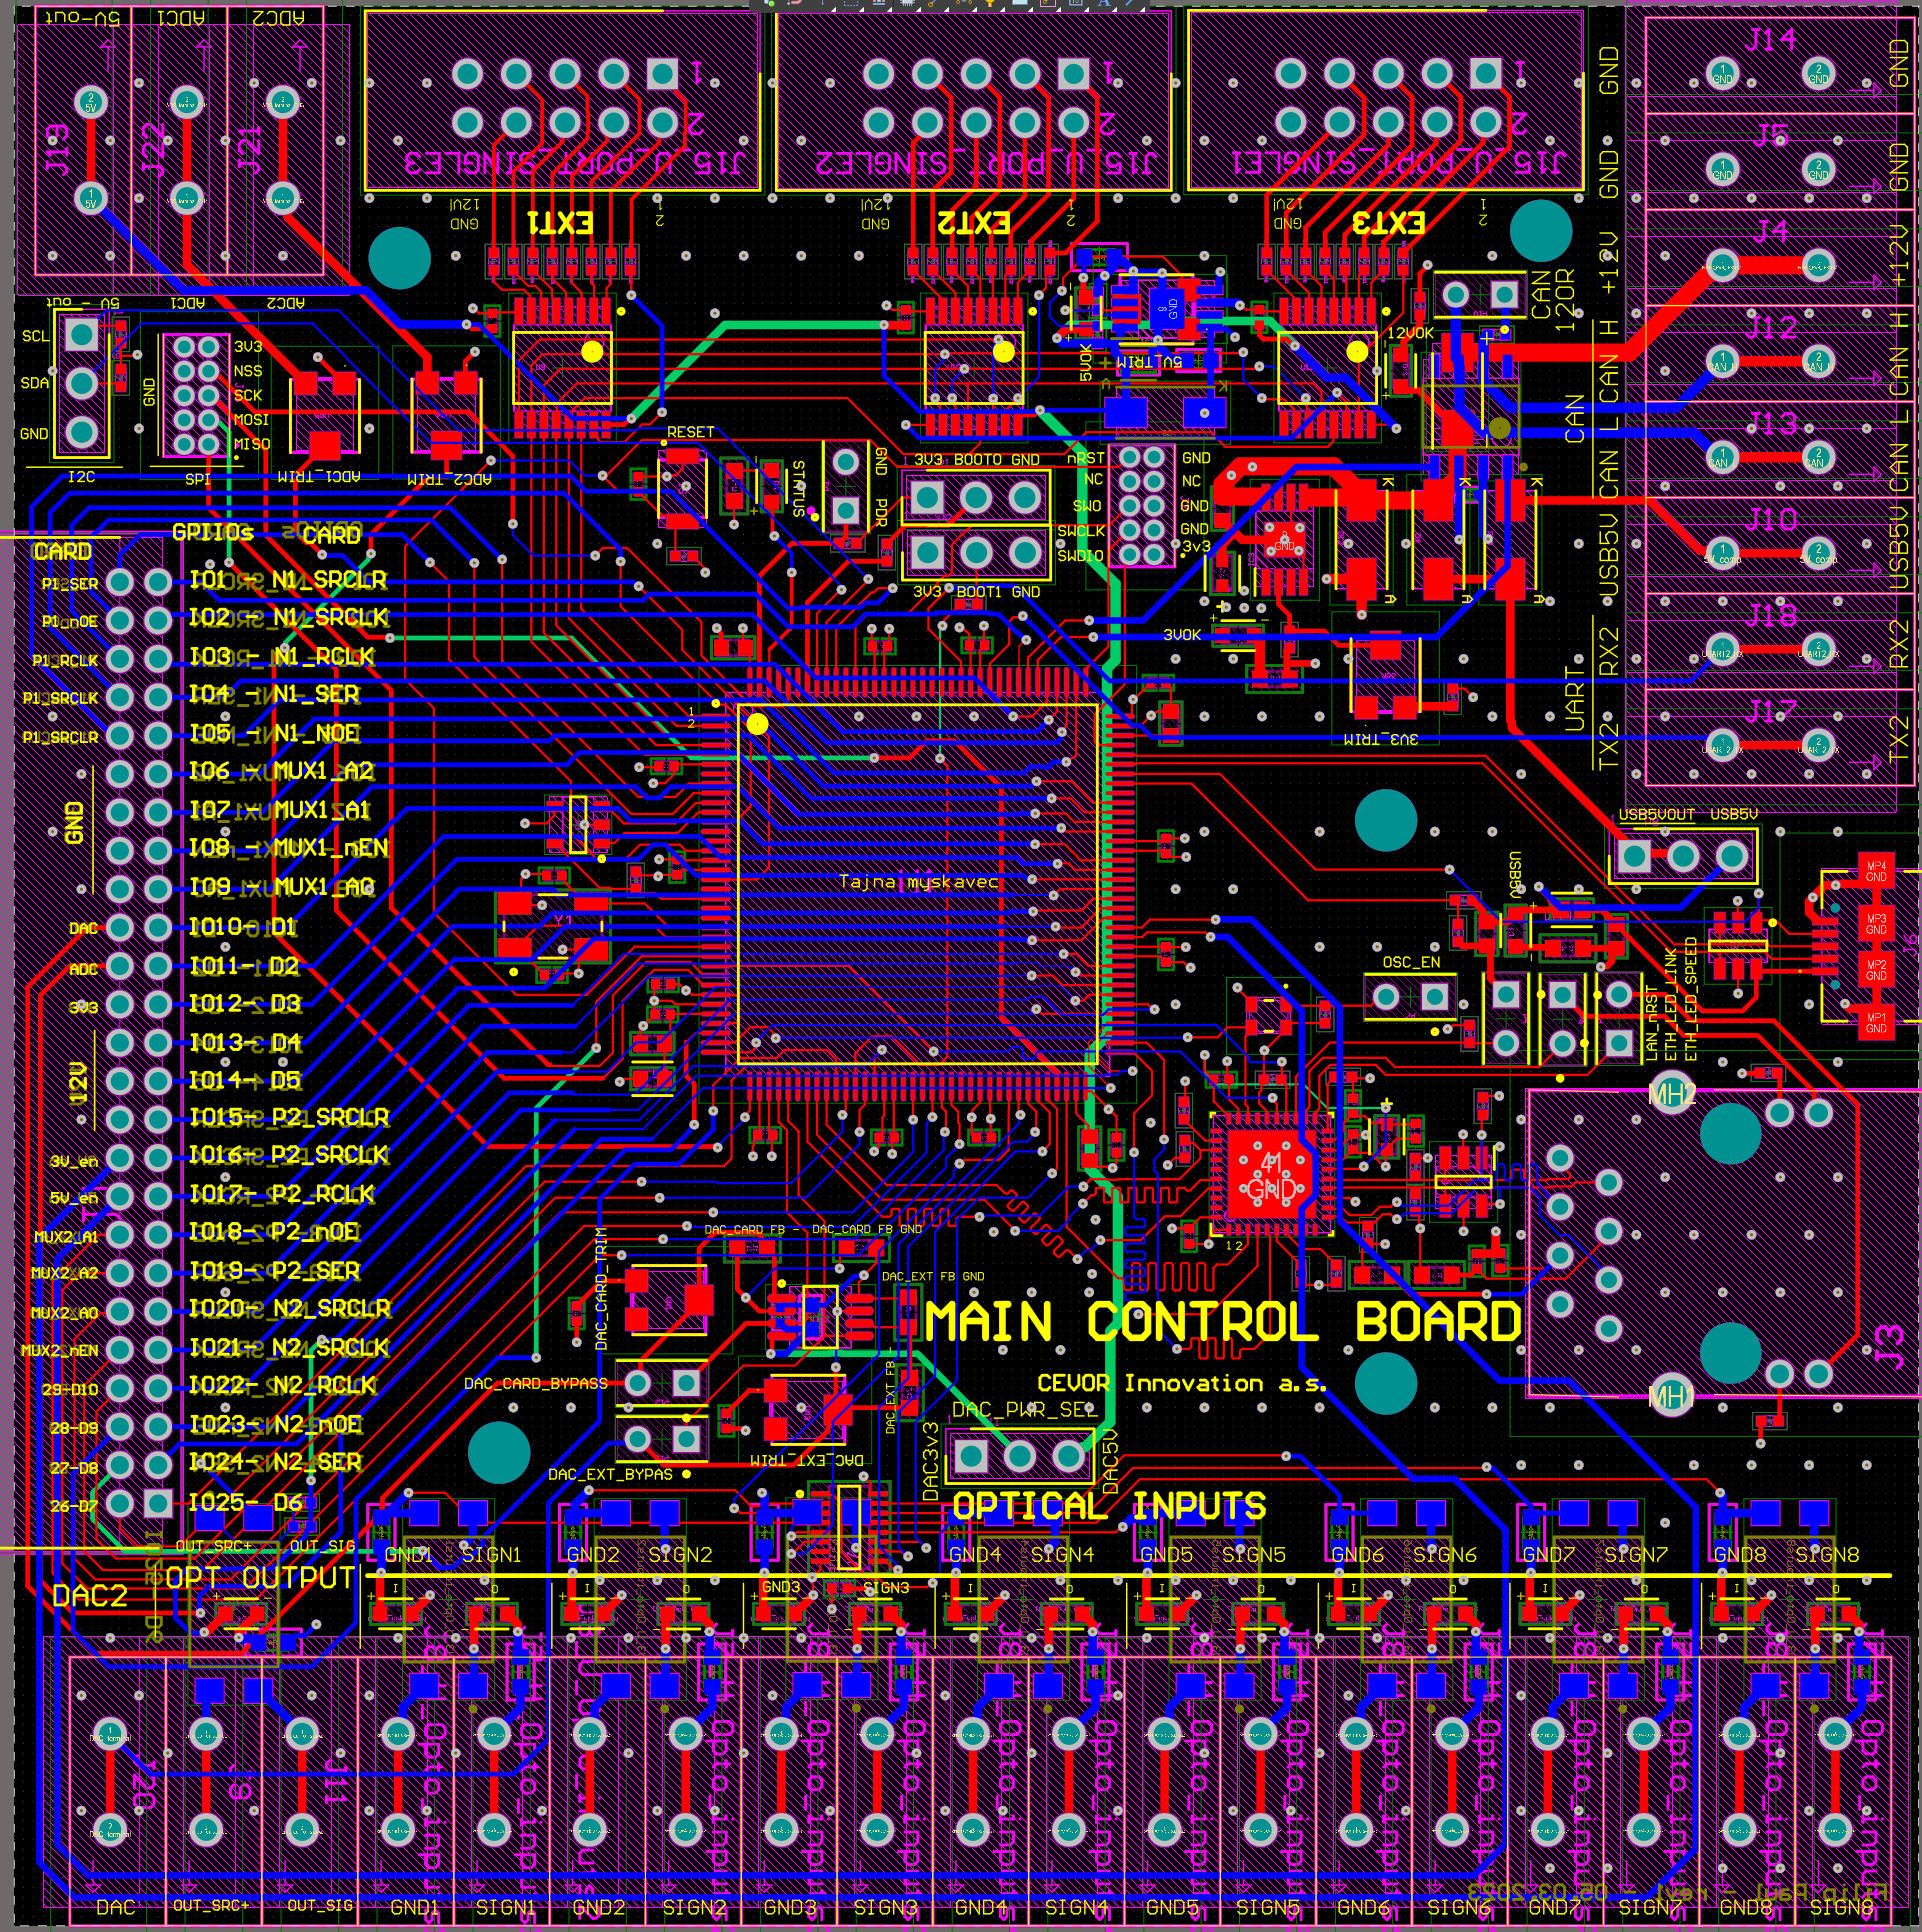
\includegraphics[width = 1\textwidth]{obrazky/all_layers_no_poly_control.png}
    \caption{Návrh PCB ovládací karty - všechny vrstvy bez polygonů}
    \label{fig:Všechny vrstvy bez polygonů control}
\end{figure}
    





    %\subsection{Návrh PCB}
    %Tady bude sekce o návrhu PCB. Zatím není navrženo.
    %Ve výrobě jsou měřící karty, které by snad i s osazením měly být hotové do obhajoby semestrální práce.
    %Poté bude měřící karta otestována jejich funkčnost pomocí NUCLEO prototypových kitů.
    %Po verifikaci funkčnosti bude vyrobena ovládací karta.
    %Bude se pravděpodobně jednat o šestivrstvé PCB s řízenými impedancemi pro diferenciální páry.
    %    \subsubsection{USB routing}
    %Nějaký stručný popis vlivu impedance cesty na rychlost USB...
    %\subsubsection{Ethernet routing}
    %Nějaký stručný popis vlivu impedance cesty na rychlost Ethernetu. Signal integrity atd..
    %\subsubsection{STM32F4 routing}
    %Vliv decoupling kondenzátorů.
    %\subsubsection{Fyzické rozměry}
    %Na rozdíl od měřících karet, kde byl kladen důraz na maximální výšku karty z důvodu roztečí bRC pinů, nejsou
    %kladeny na ovládací karty žádné omezení, protože ovládací karty budou propojeny s měřícími kartami
    %pomocí páskových vodičů. Rozměry by však měly být co nejkompaktnější. Propojit měřící karty s bRC piny pomocí
    %páskových vodičů nebylo žádoucí z důvodu vnášení chyby měření do systému.
    %\clearpage


\chapter{Algoritmizace a měřící procedury}
Jak již bylo zmíněno v kapitole o systémové koncepci a na obr.\ref{fig:Systémová koncepce}.
Jednotlivé ovládací karty jsou propojeny pomocí ethernetového rozhraní do switche.
Pro správnou funkčnost testeru je zde použit spravovatelný switch, který mimo jiné umožňuje
získat informace o své MAC tabulce. MAC tabulku společně s protokolem ARP lze využít pro
přiřazení čísla portu ethernetového switche k IP adrese připojených ovládacích karet. Tímto způsobem
lze přiřadit jednotlivé ovládací karty k jednotlivým řadám bRC pinů bez nutnosti dodatečné konfigurace
či různému kódování řad.\\

Z pohledu celého systému je hlavním řídícím prvkem PC aplikace. V následující části je popsán Komunikační
protokol, který je použit pro komunikaci mezi PC aplikací a ovládacími kartami.

\section{Komunikační protokol ovládacích karet}
Komunikační protokol je založen na ASCII příkazech a je tak relativně čitelný pro člověka.
Jednotlivé příkazy protokolu jsou přenášeny pomocí TCP/IP rámců (port 23) v případě ethernetového rozhraní nebo
pomocí Virtuálního COM portu v případě USB rozhraní. Pro obě možnosti připojení se protokol neliší.\\

Jednotlivé příkazy jsou vyhodnocovány po obdržení znaku CR (ASCII 0x0D), LF (ACII 0x0A) nebo jejich libovolnou kombinací. Odpovědi
z ovládacích karet jsou zakončeny znakem LF. Ovládací karta je určena obecně k ovládání více modulů než pouze měřících karet. Nicméně pro účely
diplomové práce jsou diskutovány pouze příkazy vztahující se k měřícím kartám. Každý příkaz vztahující se k měřícím kartám obsahuje prefix 80\_IO\_CARD.
Jednotlivé parametry příkazu jsou odděleny mezerou.\\

Pro každý příkaz odesílá ovládací karta odpovědi začínajícími prefixem "ERROR;"\ nebo "OK;"\ (bez uvozovek) podle toho, zda-li byl příkaz vyhodnocen úspěšně či nikoliv.
Poté následuje textová odpověď na příkaz zakončená znakem LF.
Příkazy jsou rozděleny do 3 skupin (SET READ a MEASUERE). Skupina SET slouží k nastavení parametrů měření, skupina READ slouží k čtení nastavených parametrů
a skupina MEASURE slouží k samotnému měření.\\

V následujících podkapitolách jsou popsány jednotlivé příkazy pomocí následující konvence:
\begin{itemize}
    \item Znak | značí, že je možné použít pouze jeden z uvedených parametrů.
    \item Text v uvozovkách značí nastavitelnou hodnotu do příkazu se zadává bez uvozovek a v případě desetinných čísel je použita desetinná tečka.
    \item Text mezi * je vysvětlen podrobněji v dané sekci
    
\end{itemize}

\subsection{Příkazy SET}
\subsubsection{SET DAC}
Příkaz SET DAC slouží k nastavení napětí na výstupu DAC. Protože se jedná o 12 bitový převodník, je možné nastavit pouze hodnoty napětí, které jsou násobky
napětí referenčního napětí. Pokud je zadáno napětí, které není násobkem referenčního napětí, je nastaveno nejbližší nižší napětí.
Referenční napětí ovládací karty je nastaveno při kalibraci příkazem SET CONFIGURATION VOLTAGE\_REFERENCE. Případně je hodnotu referenčního napětí možno získat
příkazem READ CONFIGURATION VOLTAGE\_READINGS.
\begin{itemize}[leftmargin=*]
    \item \textbf{Obecný tvar:} 80\_IO\_CARD SET DAC "Napětí ve V"
    \item \textbf{Příklad:}\\
    -> 80\_IO\_CARD SET DAC 2.75\\
    <- OK;DAC: 3398, discretized Value in Volts:2.74959
    \item \textbf{Interpretace odpovědi:} Tato odpověď byla obdržena při referenčním napětí 3.314400V. Hodnota 3398 je bitová hodnota, která je zapsána do registru DAC a
    hodnota 2.74959 je odpovídající hodnota napětí.
\end{itemize}

\subsubsection{SET SHIFT\_REGISTER}
Příkaz SET SHIFT\_REGISTER slouží k nastavení výstupní hodnoty posuvného registru či celé skupiny posuvných registrů.
Prvním parametrem příkazu je volba skupiny posuvných registrů.
Relevantní skupiny posuvných registrů pro diplomovou práci jsou IO1TO40\_OUTPUTS, IO41TO80\_OUTPUTS, IO1TO40\_IMPEDANCES a IO41TO80\_IMPEDANCES.
Správnou kombinací výstupů těchto posuvných registrů lze nastavit jakýkoliv bRC pin do vysoké či nízké impedance a případně i výstupní hodnotu napětí.\\

Druhým parametrem je volba způsobu zadání výstupní hodnoty registrů. K dispozici jsou následující možnosti: VALUE a DO\_N\_SHIFTS.
V případě možnosti VALUE následuje decimální hodnota jejíž bitové vyjádření reprezentuje stavy jednotlivých výstupů posuvných registrů.
Každý ze skupin registrů má svoji endianitu, kterou lze zjistit z příkazu READ CONFIGURATION SHIFT\_REGISTERS (podrobněji popsáno dále). 
Druhou možností je využití parametru DO\_N\_SHIFTS, který posune celý obsah posuvného registru o zadaný počet bitů v pravo či vlevo v závislosti na endianitě registru.

\begin{itemize}[leftmargin=*]
    \item \textbf{Obecný tvar:} 80\_IO\_CARD SET SHIFT\_REGISTER *registr* *způsob* "Hodnota"
    \item \textbf{*registr*:} IO1TO40\_OUTPUTS, IO41TO80\_OUTPUTS,\\
    IO1TO40\_IMPEDANCES, IO41TO80\_IMPEDANCES
    \item \textbf{*způsob*:} VALUE, DO\_N\_SHIFTS
    \item \textbf{Příklad:}\\
    -> 80\_IO\_CARD SET SHIFT\_REGISTER IO1TO40\_IMPEDANCES VALUE 4\\
    <- OK;Setting Register:IO1TO40\_IMPEDANCES to:4\\
    -> 80\_IO\_CARD SET SHIFT\_REGISTER IO1TO40\_IMPEDANCES DO\_N\_SHIFTS 4\\
    <- OK;Setting Register:IO1TO4\_IMPEDANCES to:16
    \item \textbf{Interpretace odpovědi:} Obecně lze vždy v odpovědi nalézt nový stav registru po provedení požadované operace.
\end{itemize}

\subsubsection{SET CONFIGURATION}
Příkazy v této skupině obecně slouží k nastavení stavových hodnot, kalibračních hodnot případně nastavení způsobu
měření určitých hodnot. Hodnoty, které potřebují být nastaveny pomocí prefixu SET CONFIGURATION jsou popsány v sekcích pro které jsou tyto hodnoty používány.
Ukázky vybraných hodnot, které lze nastavit pomocí příkazu SET CONFIGURATION jsou uvedeny například v sekci READ CONFIGURATION.

\begin{itemize}[leftmargin=*]
    \item \textbf{Obecný tvar:} 80\_IO\_CARD SET CONFIGURATION *Název konfigurace* "Hodnota"
    \item \textbf{*Název konfigurace*:} Popsáno v sekcích pro které jsou hodnoty používány.
    \item \textbf{Příklad:}\\
    -> 80\_IO\_CARD SET CONFIGURATION VOLTAGE\_REFERENCE 3.3144\\
    <- OK;VOLTAGE\_REFERENCE set to:3.314400
    \item \textbf{Interpretace odpovědi:} Obecně lze vždy v odpovědi nalézt potvrzení o nastavení hodnoty.
\end{itemize}

\subsection{Příkazy READ}
\subsubsection{READ MUX}
Příkaz READ MUX umožňuje číst hodnoty z multiplexerů umístěných na ovládací kartě. Příkaz se skládá ze 2 parametrů. Prvním parametrem je volba
skupiny multiplexerů. Pro ovládací kartu jsou k dispozici 2 skupiny (MUXES\_1TO40 a MUXES\_41TO80). Druhým parametrem je volba podoby obdržené hodnoty.
První možností je přečíst hodnotu celé skupiny multiplexeru za použití parametru ALL. Výsledkem tohoto příkazu je 40bitové číslo v decimální podobě,
kde každý bit reprezentuje stav jednoho bRC pinu připojeného ke zvolenému multiplexeru. 40bitová hodnota je vztažena k endianitě multiplexeru, kterou lze zjistit
příkazem 80\_IO\_CARD READ CONFIGURATION MULTIPLEXERS.
Druhou možností je zadat přímo číslo pinu, jehož stav chceme zjistit. Výsledkem tohoto příkazu je 1bitová hodnota v decimální podobě.
\begin{itemize}[leftmargin=*]
    \item \textbf{Obecný tvar:} 80\_IO\_CARD READ MUX *multiplexer* "číslo pinu"|ALL
    \item \textbf{*multiplexer*:} MUXES\_1TO40 a MUXES\_41TO80
    \item \textbf{Příklad:}\\
    -> 80\_IO\_CARD READ MUX MUXES\_1TO40 ALL\\
    <- OK;Reading MUX MUXES\_1TO40, ALL:0\\
    -> 80\_IO\_CARD READ MUX MUXES\_1TO40 1\\
    <- OK;Reading MUX: MUXES\_1TO40, address:1, value:0
    \item \textbf{Interpretace odpovědi:} V případě parametru ALL je v odpovědi obsažena 40bitová hodnota v decimální podobě. V případě zadání čísla pinu je v odpovědi obsažena 1bitová hodnota v decimální podobě.
\end{itemize}

\subsubsection{READ SHIFT\_REGISTER}
Tento příkaz slouží k získání aktuální hodnoty shiftregistru. Jediným parametrem tohoto příkazu je jméno skupiny shiftregistru.

\begin{itemize}[leftmargin=*]
    \item \textbf{Obecný tvar:} 80\_IO\_CARD READ MUX *register*
    \item \textbf{*register*:} IO1TO40\_OUTPUTS, IO41TO80\_OUTPUTS,\\
    IO1TO40\_IMPEDANCES, IO41TO80\_IMPEDANCES
    \item \textbf{Příklad:}\\
    -> 80\_IO\_CARD READ SHIFT\_REGISTER IO1TO40\_OUTPUTS\\
    <- OK;Reading Register IO1TO40\_OUTPUTS, value:1099511627775\\
    \item \textbf{Interpretace odpovědi:} V odpovědi je obsažena 40bitová hodnota v decimální podobě,
    kde jednotlivé bity této hodnoty značí aktuální výstupní hodnotu shiftregistru v závislosti na jeho endianitě.
    V případě výpadku napájení se může stát, že hodnota shiftregistru nebude odpovídat skutečnému stavu výstupních pinů.
\end{itemize}


\subsubsection{READ CONFIGURATION}
Příkaz READ CONFIGURATION slouží k získání konfigurace ovládací karty. Ovládací karta obsahuje poměrně obsáhlé množství konfigurací.
V této sekci jsou popsány pouze ty konfigurace, které jsou využívány v diplomové práci. Některé vyčtené tímto příkazem nastavovat
pomocí příkazu SET CONFIGURATION.
\begin{itemize}[leftmargin=*]
    \item \textbf{Obecný tvar:} 80\_IO\_CARD READ CONFIGURATION *konfigurace*
    \item \textbf{Příklad SHIFT\_REGISTERS:}\\
    -> 80\_IO\_CARD READ CONFIGURATION SHIFT\_REGISTERS\\
    <- OK;IO1TO40\_OUTPUTS:(length:40,endianity:1,value:1099511627775);\\
    IO41TO80\_OUTPUTS:(length:40,endianity:0,value:0);\\
    IO1TO40\_IMPEDANCES:(length:40,endianity:1,value:1);\\
    IO41TO80\_IMPEDANCES:(length:40,endianity:0,value:0);
    \item \textbf{Interpretace odpovědi:} V odpovědi jsou obsaženy veškeré informace o konfiguraci posuvných registrů.
    \item \textbf{Příklad MULTIPLEXERS:}\\
    -> 80\_IO\_CARD READ CONFIGURATION MULTIPLEXERS\\
    <- OK;MUXES\_1TO40:(bits:8,paralel:5,endianity:0,value:0);\\
    MUXES\_41TO80:(bits:8,paralel:5,endianity:0,value:0);
    \item \textbf{Interpretace odpovědi:} V odpovědi jsou obsaženy veškeré informace o konfiguraci multiplexerů.
    \item \textbf{Příklad VOLTAGE\_READINGS:}\\
    -> 80\_IO\_CARD READ CONFIGURATION VOLTAGE\_READINGS\\
    <- OK;DAC\_RAMP\_DIRECTION:0;\\
    DAC\_RAMP\_MIN\_VALUE\_VALUE:0;\\
    DAC\_RAMP\_MAX\_VALUE\_VALUE:4095;\\
    DAC\_RAMP\_STEP:1;\\
    DAC\_RAMP\_DELAY\_2500\_NS:2;\\
    VOLTAGE\_READ\_AVERAGES:2;\\
    VOLTAGE\_REFERENCE:3.314400;
    \item \textbf{Interpretace odpovědi:} V odpovědi jsou obsaženy veškeré nastavitelné parametry, které se využívají při měření napětí na jednotlivých pinech příkazy MEASURE.
\end{itemize}





\subsection{Příkazy MEASURE} \label{measure commands}
\subsubsection{MEASURE VOLTAGE}
Příkaz MEASURE VOLTAGE slouží k měření napětí na určitém bRC pinu či pinech. V případě použití parametru ALL je změřeno napětí na všech 80 pinech měřící karty.
V případě, že je místo parametru ALL zadáno číslo tak příkaz vrátí hodnotu napětí na daném pinu.\\

\begin{itemize}[leftmargin=*]
    \item \textbf{Obecný tvar:} 80\_IO\_CARD MEASURE VOLTAGE ALL|"číslo pinu"
    \item \textbf{Příklad ALL:}\\
    -> 80\_IO\_CARD MEASURE VOLTAGE ALL\\
    <- OK;2.965643;2.860450;2.431585;-1.000000;0.922465;........;-1.00000;-1.000000;
    \item \textbf{Interpretace odpovědi:} V odpovědi jsou obsaženy hodnoty napětí na všech 80 pinech odděleny znakem ;. "...." V příkladu značí, že výpis byl zkrácen.
    Hodnota -1 značí, že napětí je mimo rozsah měřící karty.

    \item \textbf{Příklad číslo pinu:}\\
    -> 80\_IO\_CARD MEASURE VOLTAGE 3
    <- OK;Voltage:2.128143\\
    \item \textbf{Interpretace odpovědi:} V odpovědi je obsaženo napětí na pinu 3 (číslováno od 0). V případě, že napětí je mimo rozsah měřící karty, tak příkaz vrátí hodnotu -1.
\end{itemize}

Proces měření napětí lze konfigurovat pomocí příkazů ze skupiny SET CONFIGURATION. Následující část popisuje vliv vybraných parametrů.
Měření napětí probíhá pomocí porovnávání nastavené hodnoty D/A převodníku s měřenou hodnotou napětí na bRC pinu. V reálném zapojení je tohoto dosaženo pomocí komparátoru.
Výstup komparátoru je z důvodu velkého množství pinů multiplexován na digitální vstup mikrokontroléru (Obr.\ref{fig: bRC pin voltage measurement}). 

\begin{figure}[ht!]
    \centering
    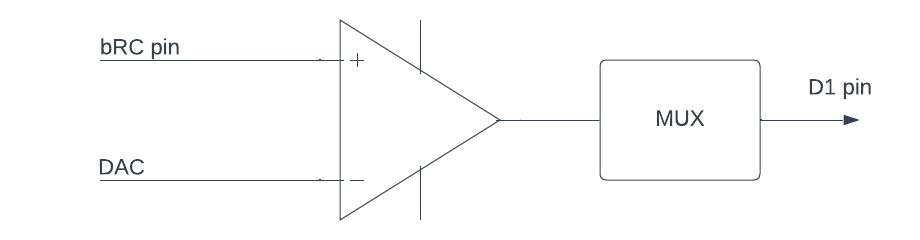
\includegraphics[width = 0.9\textwidth]{obrazky/Voltage_measurement_example.png}
    \caption{Zjednodušené schéma zapojení pro měření napětí na bRC pinu}
    \label{fig: bRC pin voltage measurement}
\end{figure}

Měření popsána v této sekci byla provedena na reálné měřící kartě, kde výstup multiplexeru pro měřený bRC pin je přiveden na pin D1 olvádací karty. Měření byla provedena pomocí
osciloskopu KEYSIGHT DSOX1204A a digitálního 6 a 1/2 místného multimetru GWINSTEK GDM-9061.
Kde jednotlivé průběhy napětí jsou následně zpracovány pomocí programu MATLAB.\\

Na obrázku \ref{fig: bRC pin voltage measurement DACRAMP1} je zobrazen průběh napětí jednotlivých uzlů z obr. \ref{fig: bRC pin voltage measurement}. Modře je znázorněna měřená hodnota napětí na bRC pinu,
která má podle multimetru hodnotu 2.1475V, přičemž příkaz vrátil hodnotu napětí 2.1275V. Tato hodnota je závislá na nastavení napěťové reference příkazem 80\_PIN\_CARD SET CONFIGURATION VOTAGE\_REFERENCE.\\

Červeně je zobrazena hodnota napětí na výstupu D/A převodníku a zeleně je znázorněn výstup multiplexeru. 
Každá z následujících diskutovaných konfigurací v této sekci začíná prefixem 80\_PIN\_CARD SET CONFIGURATION, přičemž je tento prefix vynecháván.

\begin{figure}[ht!]
    \centering
    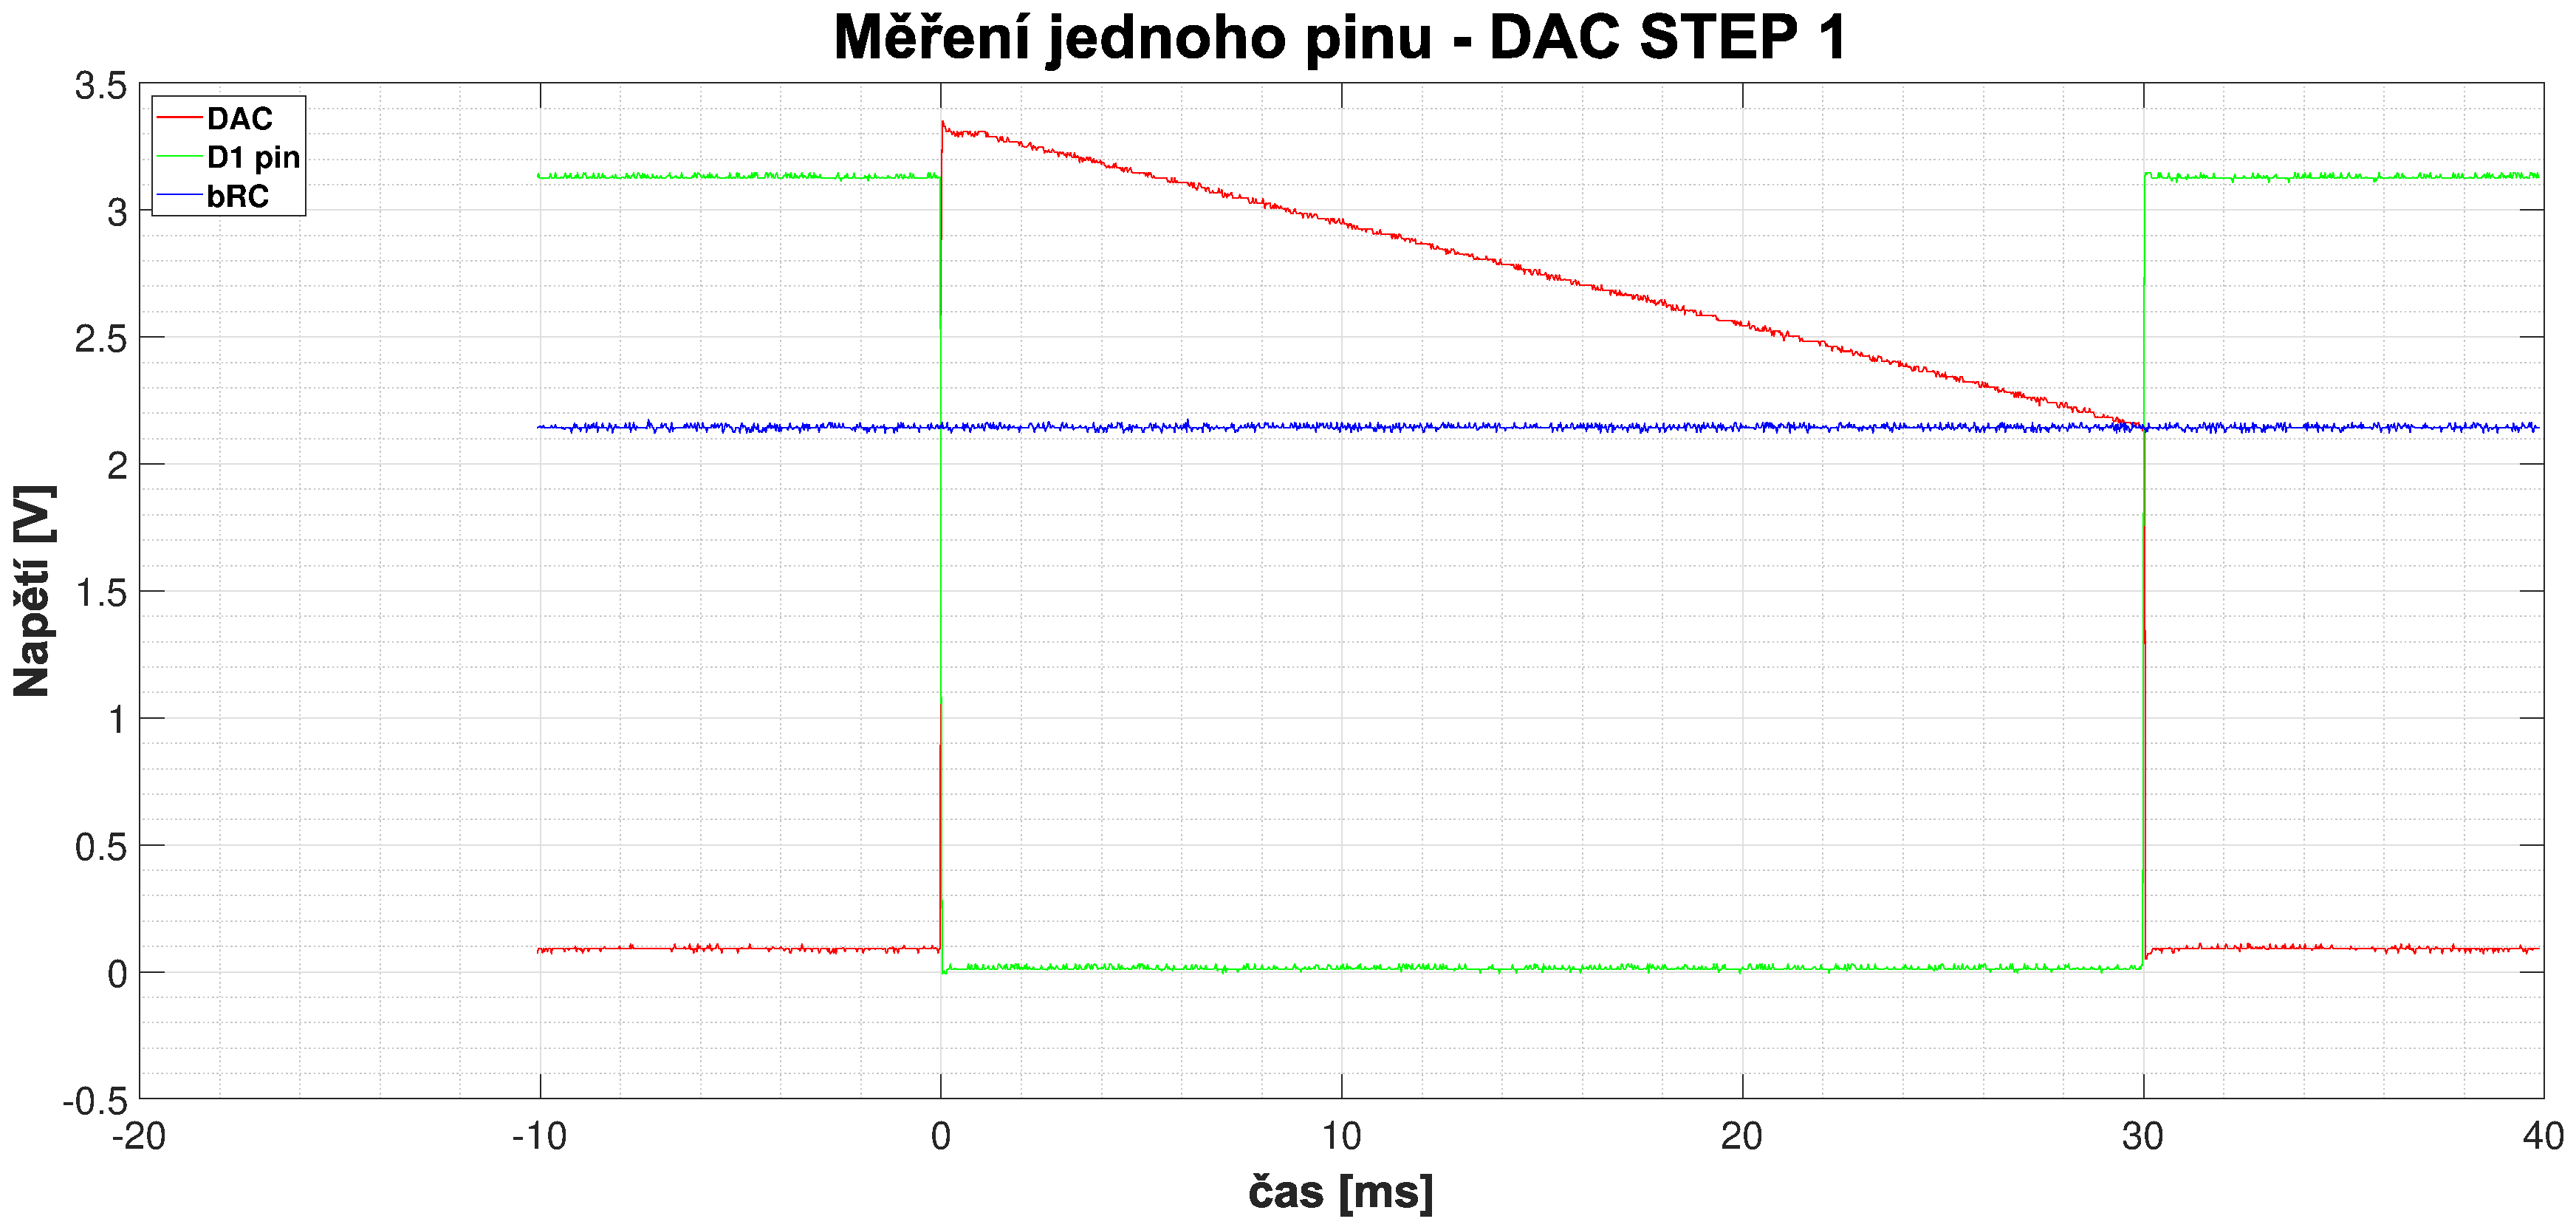
\includegraphics[width = 0.9\textwidth]{obrazky/matlab_generated/pin_step1.eps}
    \caption{Časové průběhy napětí - měření napětí na bRC pinu (DAC\_RAMP = 1)}
    \label{fig: bRC pin voltage measurement DACRAMP1}
\end{figure}

Měření napětí probíhá tak, že se na D/A převodníku nastavují sestupně (případně vzestupně v závislosti na konfiguraci DAC\_RAMP\_DIRECTION) hodnoty napětí. Při každém kroku se kontroluje,
zda nedošlo k překlopení napěťové úrovně na výstupu komparátoru (respektive multiplexeru - D1 pin).
Detekce překlopení probíhá tak, že se vyčítá N-krát (lze nastavit konfigurací VOLTAGE\_READ\_AVERAGES) logická hodnota na pinu D1.
Pokud je alespoň polovina z takto vyčtených hodnot opačné logické úrovně než logická úroveň pinu D1 na počátku měření,
tak se přepočte aktuálně nastavená hodnota registru D/A převodníku na napětí a toto napětí se odešle do PC aplikace.
Detekce překlopení komparátoru je patrná na obrázku \ref{fig: bRC pin voltage measurement DACRAMP1}
přibližně v čase 30\,ms.

\begin{figure}[ht!]
    \centering
    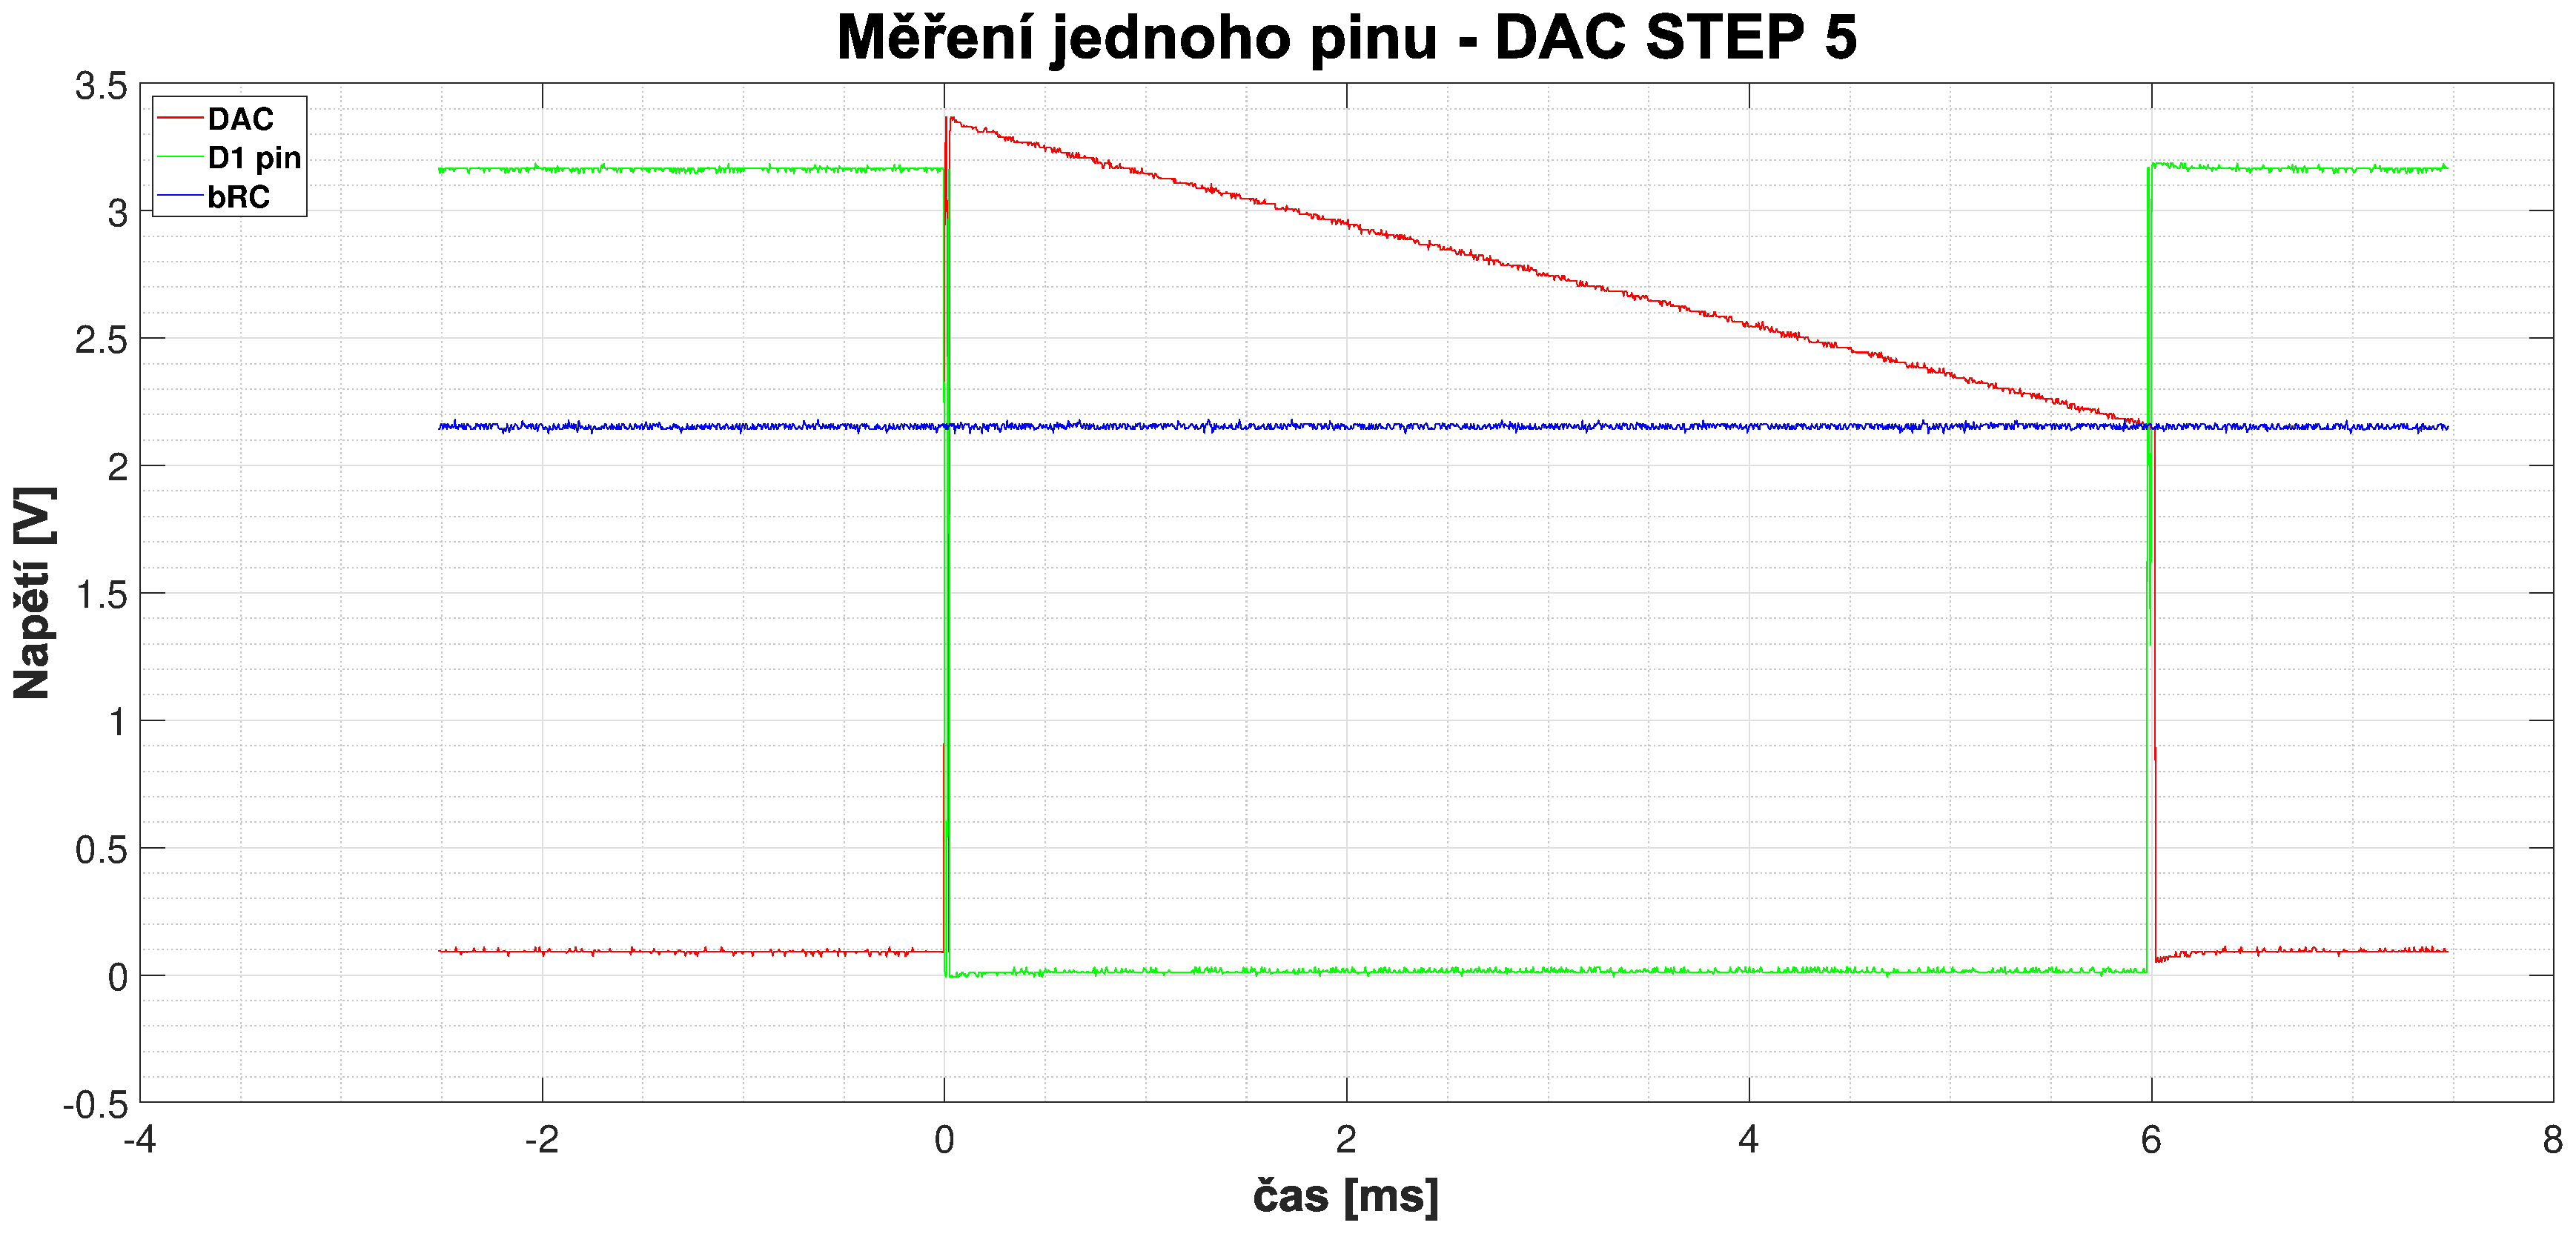
\includegraphics[width = 0.9\textwidth]{obrazky/matlab_generated/pin_step5.eps}
    \caption{Časové průběhy napětí - měření napětí na bRC pinu (DAC\_RAMP = 5)}
    \label{fig: bRC pin voltage measurement DACRAMP5}
\end{figure}

Další nastavitelnou konfigurací je DAC\_RAMP\_STEP, která udává bitový krok rampy D/A převodníku. Takto lze měření urychlit za cenu snížení přesnosti.
Na obrázku \ref{fig: bRC pin voltage measurement DACRAMP5} je zobrazen průběh napětí při nastavení DAC\_RAMP\_STEP = 5. Touto změnou
bylo dosaženo změření stejného napětí jako v předchozím bodě přibližně za 6\,ms.\\

Z obrázků \ref{fig: bRC pin voltage measurement DACRAMP1} a \ref{fig: bRC pin voltage measurement DACRAMP5} lze dedukovat, že celkový čas je závislý 
na měřeném napětí. V případě, že je zvolena sestupná rampa a měřené napětí je nulové budou průběhy vypadat následovně:

\begin{figure}[ht!]
    \centering
    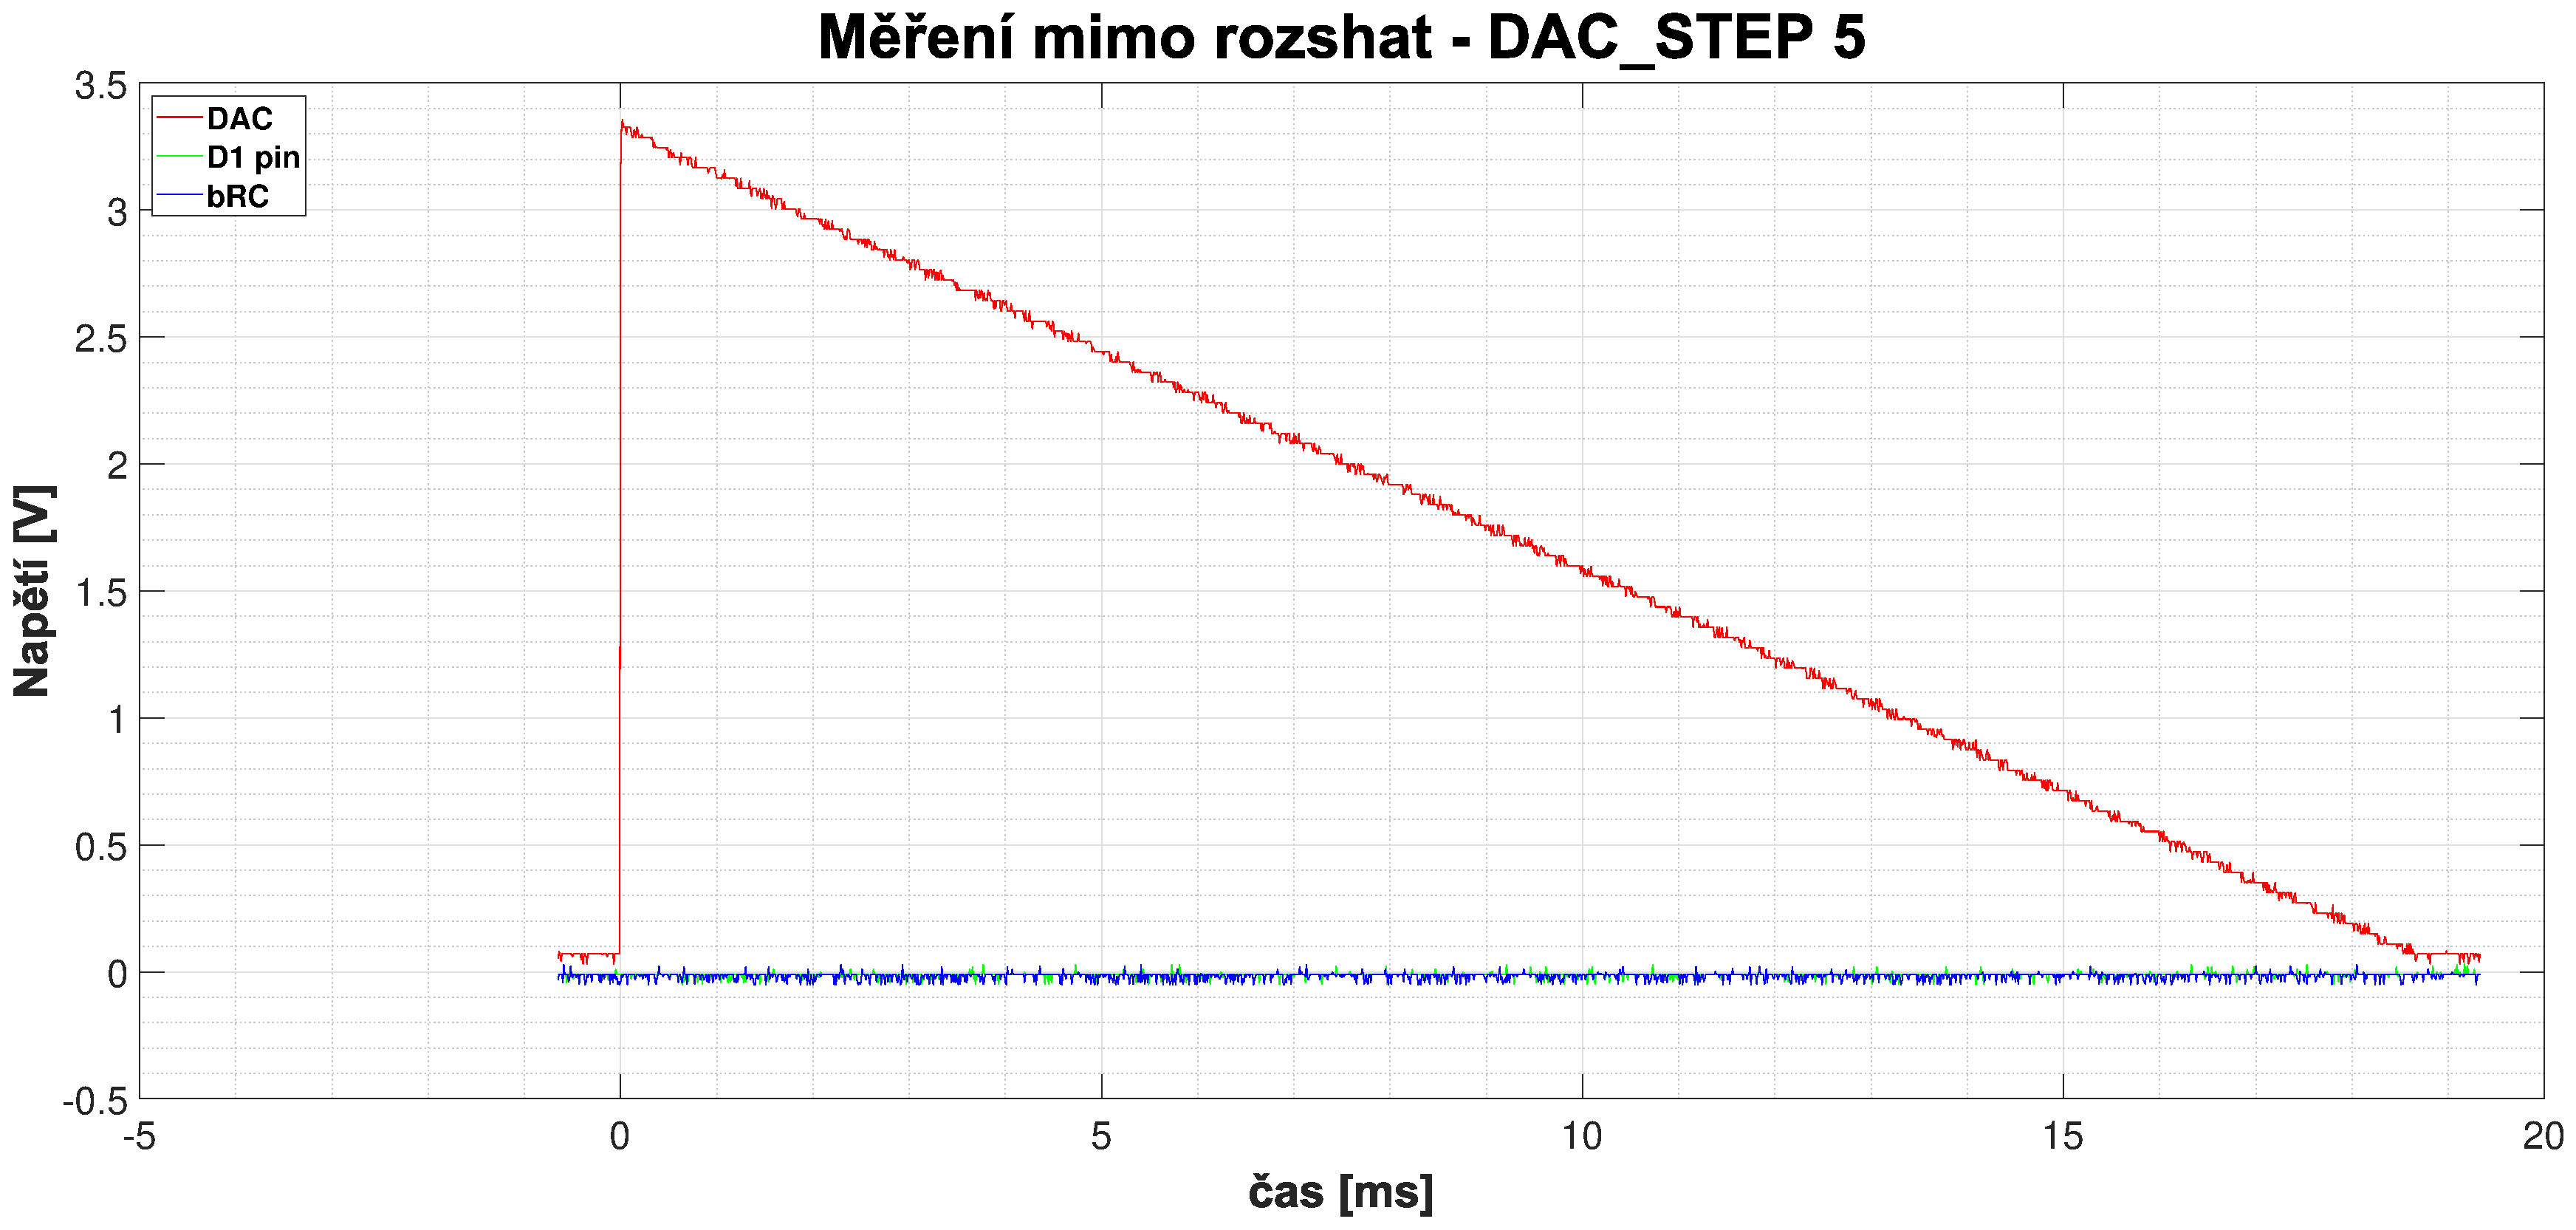
\includegraphics[width = 0.9\textwidth]{obrazky/matlab_generated/pin_out_of_range.eps}
    \caption{Časové průběhy napětí - měření nízkého napětí na bRC pinu (DAC\_RAMP = 5)}
    \label{fig: bRC pin voltage measurement low Voltage}
\end{figure}

Na obrázku \ref{fig: bRC pin voltage measurement low Voltage} lze pozorovat, že pokud napětí je příliš nízké, tak se výstup komparátoru nikdy nepřeklopí a 
příkaz vrátí v odpovědi hodnotu -1.
To je způsobeno tím, že D/A převodník není schopen generovat nulové napětí. Při nastavení registru D/A převodníku na 0 je na výstupu převodníku napětí přibližně 70\,mV.
Lze tak měřit pouze napětí, které je vyšší než tato dolní mez. Horní mez měření není omezena, protože napájecí napětí bRC pinů je nižší než napětí,
které je D/A převodník schopen generovat. Zároveň obrázek \ref{fig: bRC pin voltage measurement low Voltage} demonstruje přibližnou maximální dobu
měření (19ms pro DAC\_RAMP\_STEP = 5 a 95ms pro DAC\_RAMP\_STEP = 1). \\

\begin{figure}[ht!]
    \centering
    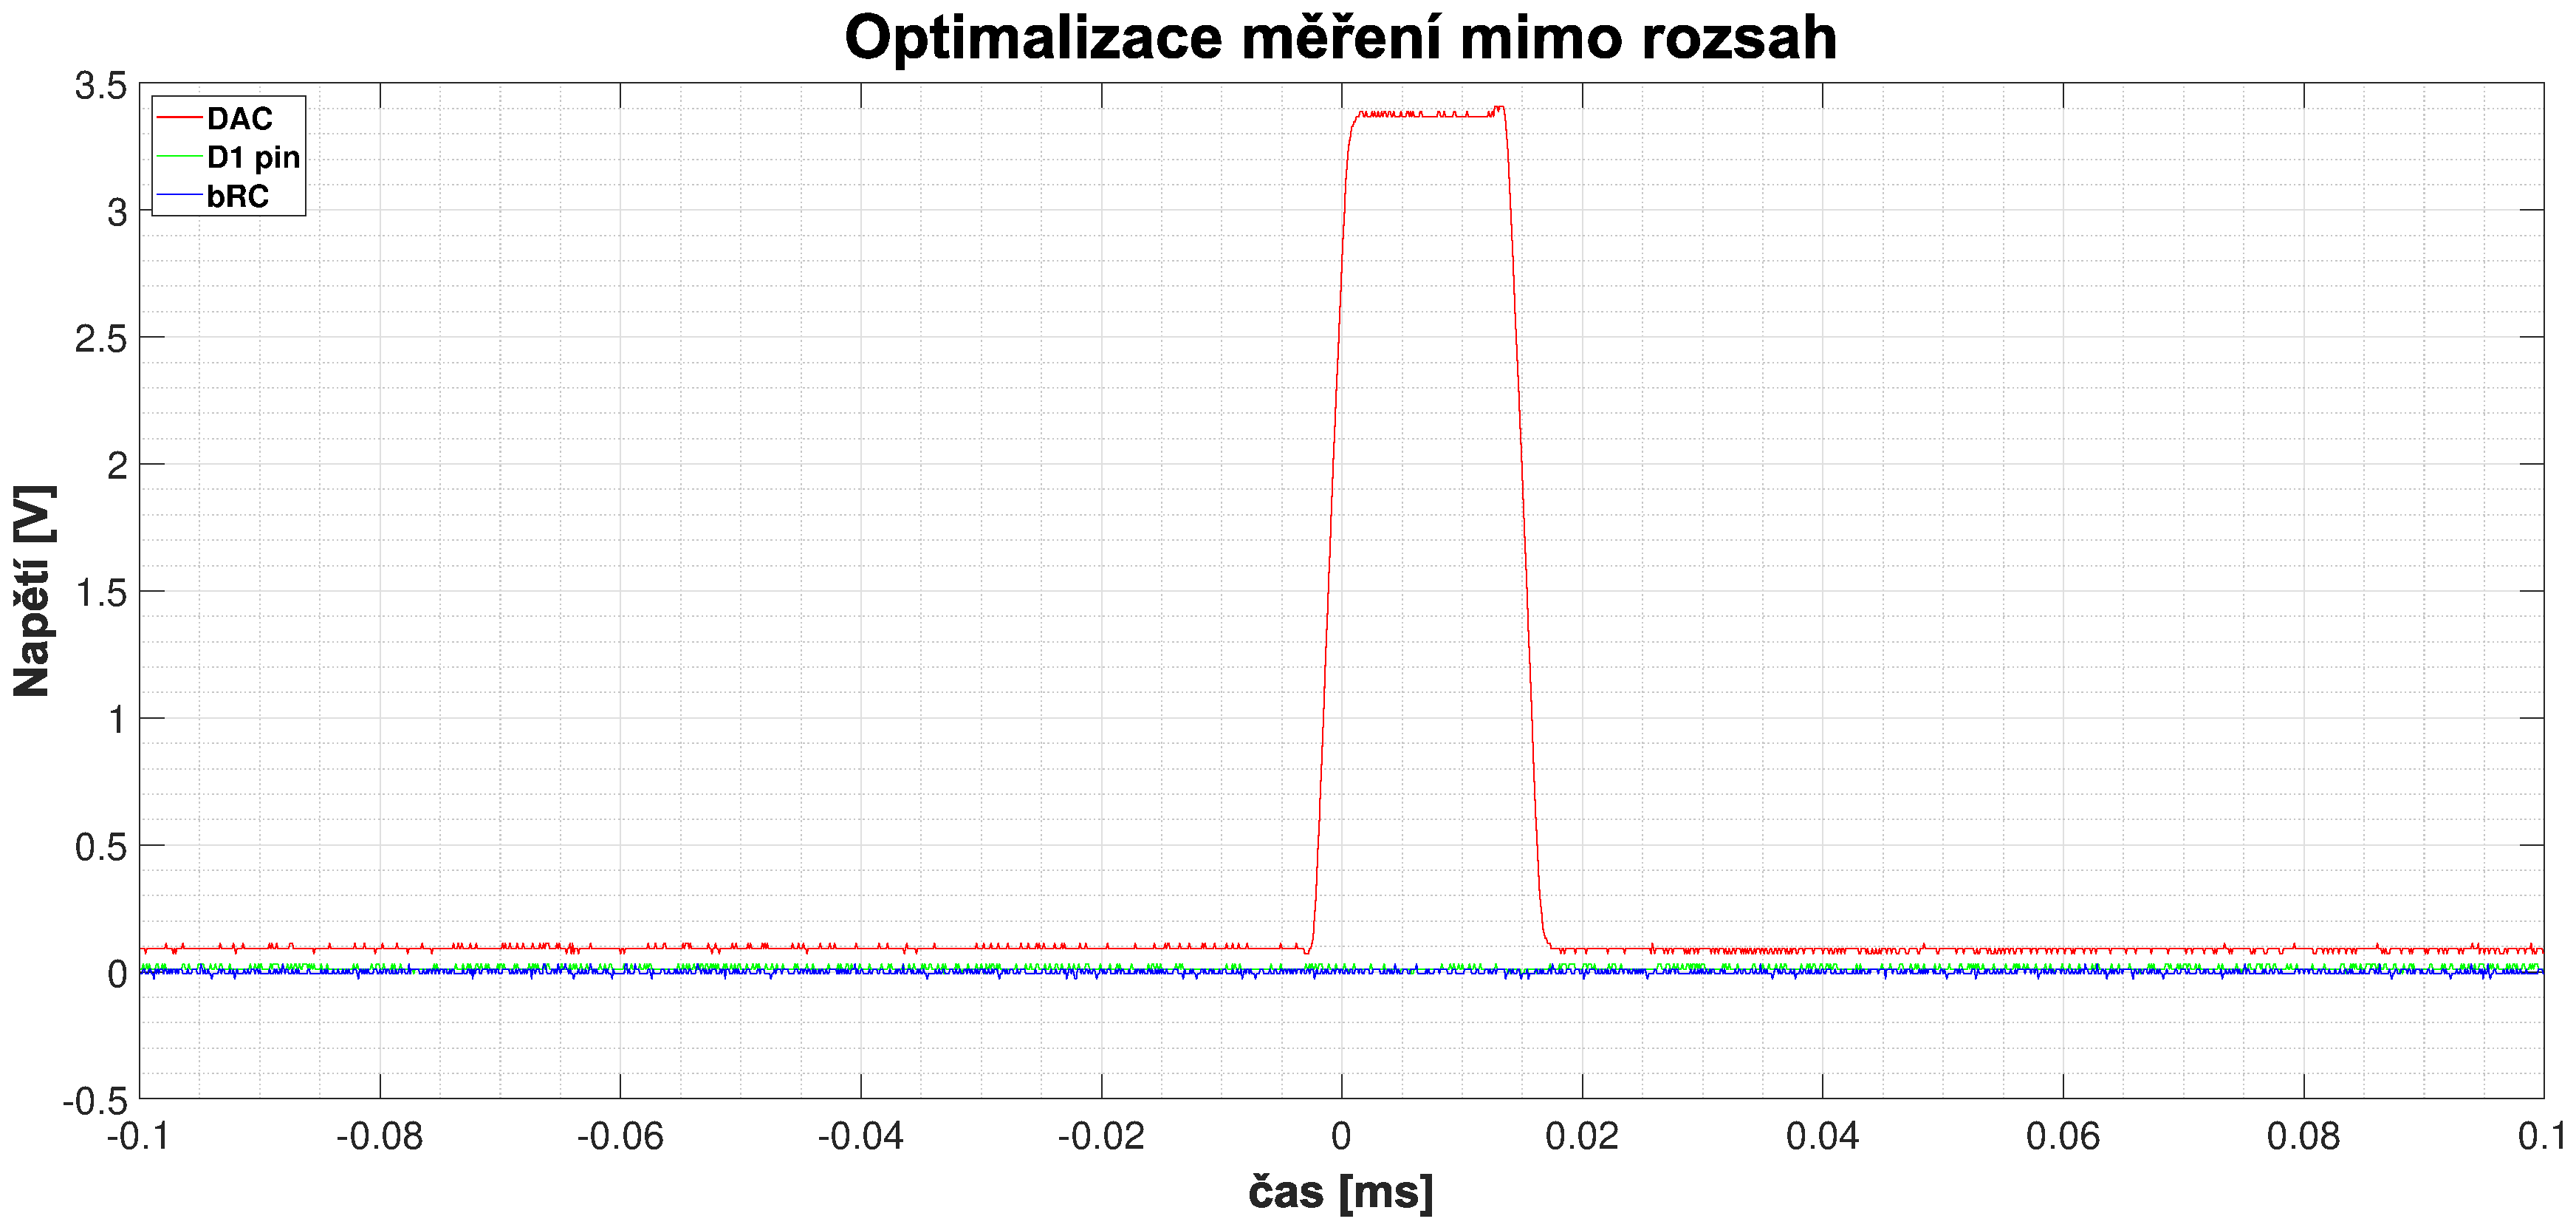
\includegraphics[width = 0.9\textwidth]{obrazky/matlab_generated/pin_out_of_range_opt.eps}
    \caption{Časové průběhy napětí - měření nízkého napětí na bRC pinu optimalizace}
    \label{fig: bRC pin voltage measurement low Voltage opt}
\end{figure}


Vzhledem k charakteru propojení bRC pinů, kde je většina pinů buď propojena tvrdým zkratem (napětí na bRC pinu blízké 3V) nebo rozpojená (napětí na pinu blízké 0V),
vzniká potřeba zkrátit čas měření napětí mimo rozsah D/A převodníku. Z tohoto důvodu je před začátkem měření nejprve změřena logická hodnota výstupu multiplexeru (D1 pin) při
nejnižší a nejvyšší napěťové hodnotě D/A převodníku. Pokud je výstup multiplexeru v obou případech stejný, tak se předpokládá, že je hodnota nižší než dolní mez D/A převodníku
a příkaz vrátí hodnotu -1. Při reálném provozu, tak nemůže nastat situace z obr. \ref{fig: bRC pin voltage measurement low Voltage}.
Měření pak probíhá podle obr. \ref{fig: bRC pin voltage measurement low Voltage opt}. Optimalizované měření pak v případě, že je měřená hodnota mimo rozsah
,trvá pouze přibližně 0.02\,ms nezávisle na použitých konfigurací.\\

Další konfigurace, které lze využít jsou DAC\_RAMP\_MAX\_VALUE\linebreak a DAC\_RAMP\_MIN\_VALUE,
které určují dolní a horní mez rampy D/A převodníku. Tímto lze zkrátit čas měření za cenu nižšího rozsahu.
Zároveň je na tyto mezní hodnoty aplikována stejná metoda jako je popsána v předchozím odstavci. Nicméně nyní dolní mez D/A převodníku nepředstavuje hardwarovou dolní mez měření,
nýbrž mez nastavenou příkazem DAC\_RAMP\_MIN\_VALUE. V případě využívání DAC\_RAMP\_MAX\_VALUE může dojít k měření hodnoty napětí mimo tuto horní mez. Protože pro funkčnost měřící karty není
nutné rozlišovat zda měřená hodnota je nad horní nebo pod dolní mezí a v obou případech vrací příkaz hodnotu -1.\\ 

Prozatím  bylo diskutováno pouze měření napětí na jednom pinu.
V případě \linebreak příkazu 80\_IO\_CARD MEASURE VOLTAGE ALL jsou změřena napětí na všech bRC pinech současně během jedné rampy
D/A převodníku (Obr. \ref{fig: bRC pin voltage measurement allpins}).

\begin{figure}[ht!]
    \centering
    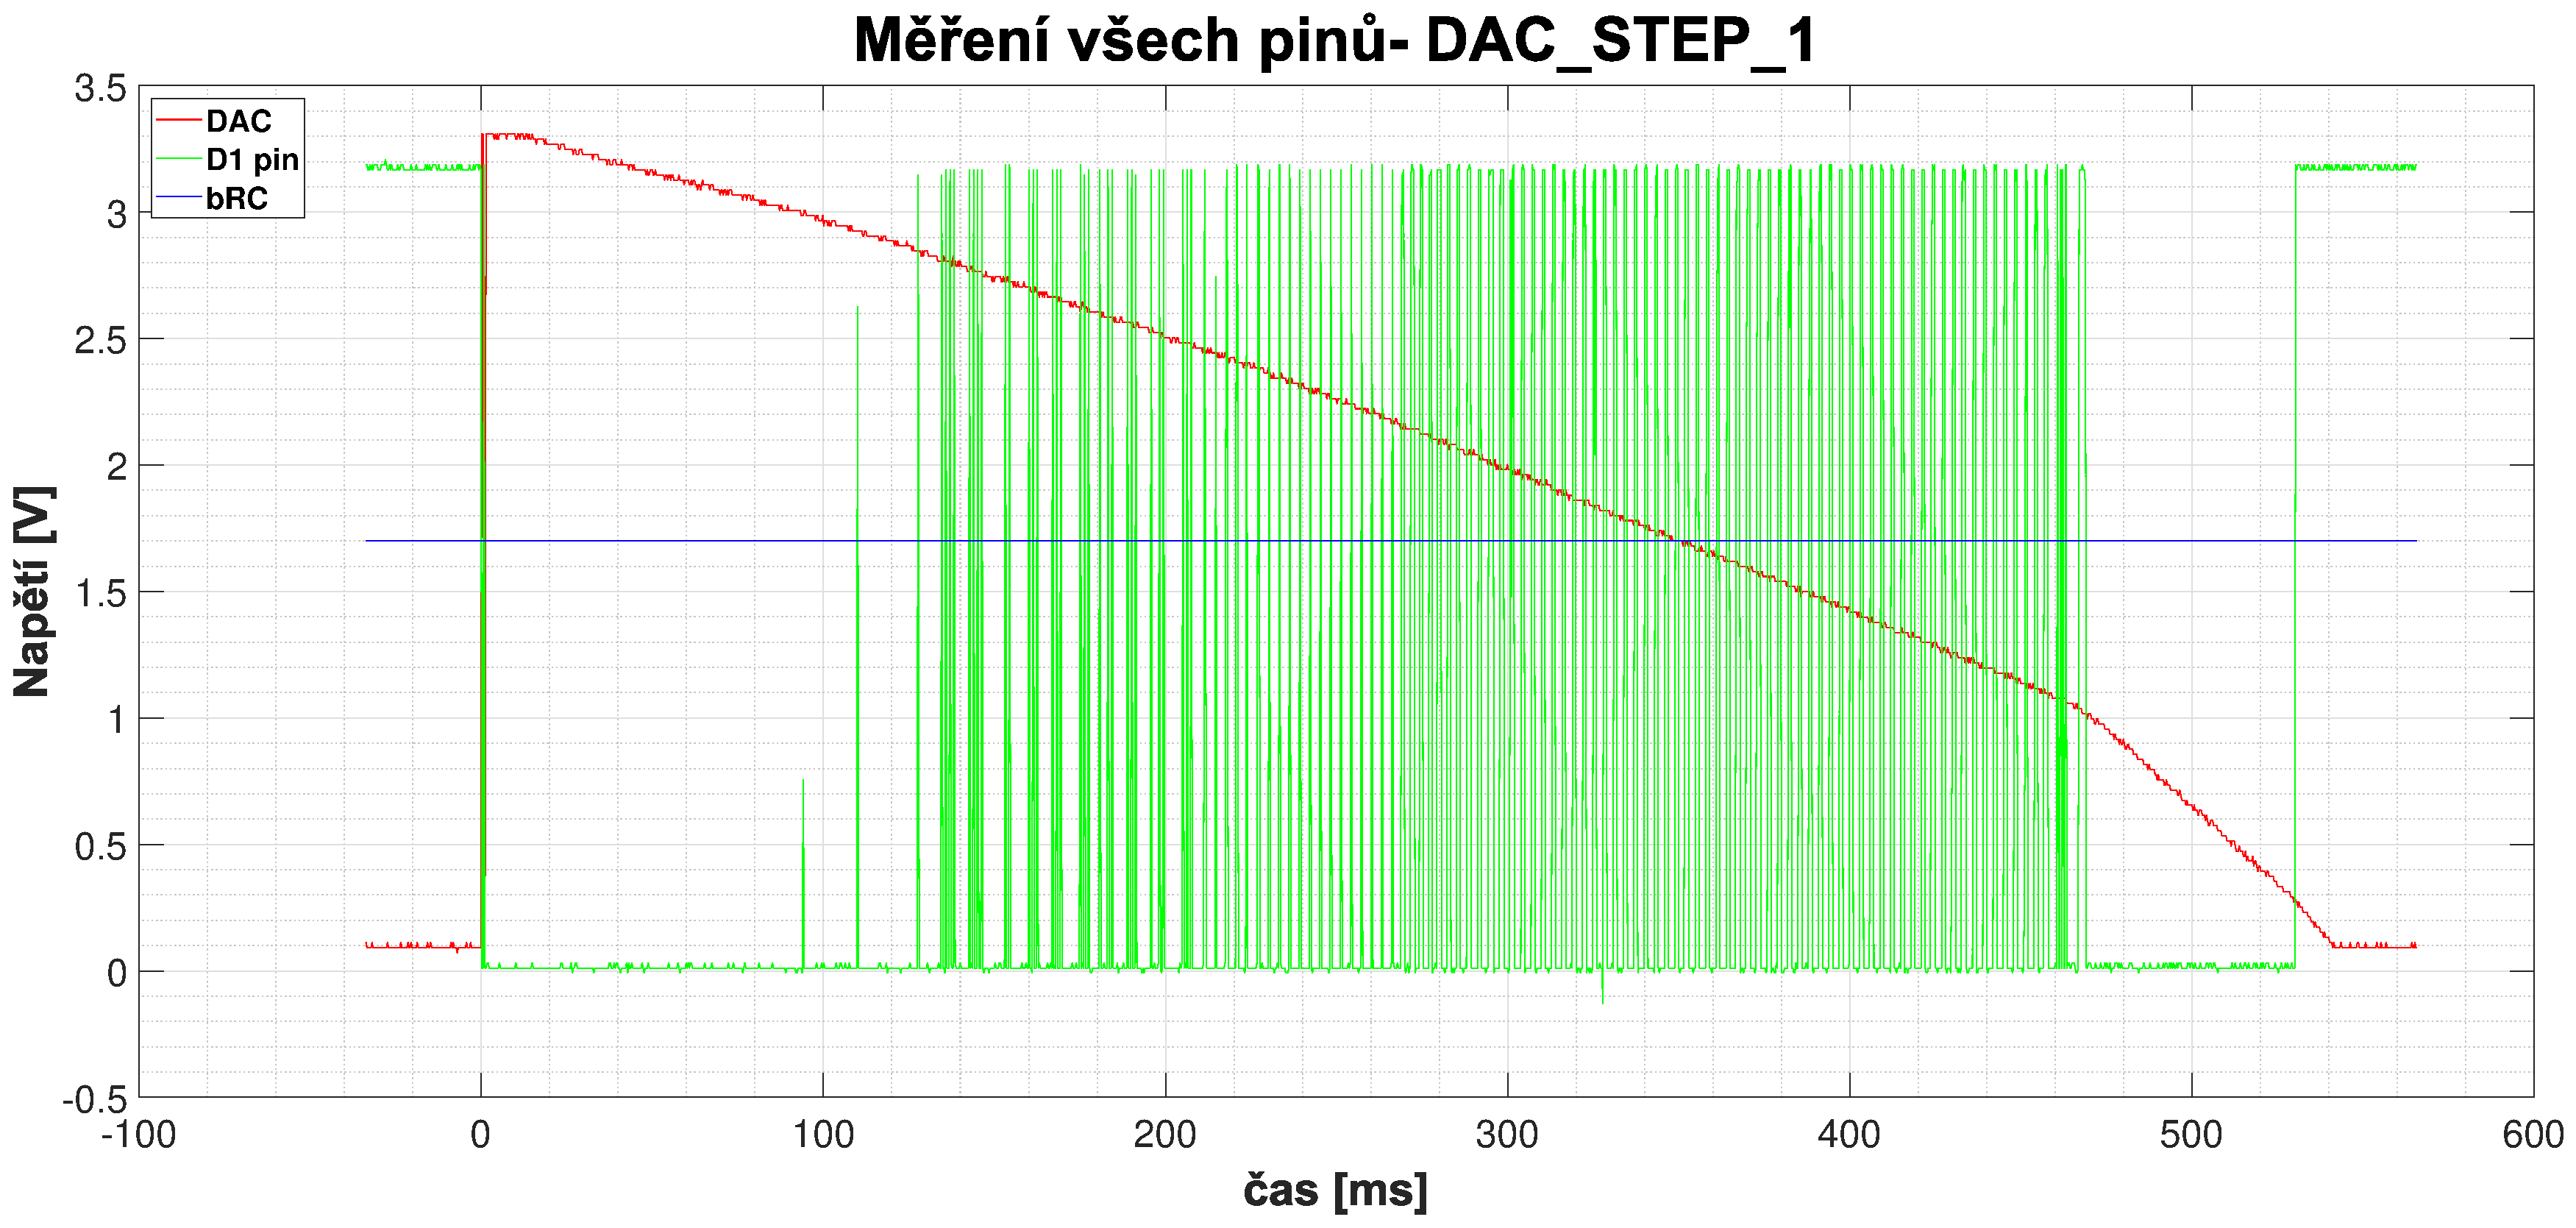
\includegraphics[width = 0.9\textwidth]{obrazky/matlab_generated/all_pins.eps}
    \caption{Časové průběhy napětí - měření napětí na všech pinech současně}
    \label{fig: bRC pin voltage measurement allpins}
\end{figure}

Měření všech pinů probíhá obdobně jako u měření jednotlivých pinů. Nejprve se u všech pinů zkontroluje, zda je měřené napětí v mezích.
Následuje D/A rampa, kde se při každém kroku kontroluje u každého pinu, zda nedošlo k překlopení komparátoru. Pokud dojde k překlopení komparátoru,
tak se uloží aktuální hodnota D/A převodníku do paměti mikrokontroléru. Pokud je pro daný pin již v paměti uložená nějaká hodnota, tak při dalším
kroku D/A rampy již nedochází ke kontrole překlopení komparátoru. To je patrné z obr. \ref{fig: bRC pin voltage measurement allpins}, kde není rampa
D/A převodníku lineární a postupně se měření urychluje s počtem již změřených pinů.\\ 

Zelený průběh napětí na D1 pinu vypadá takto, protože se jedná o výstup multiplexeru. Multiplexery jsou řízeny pomocí společné adresace, takže
se v průběhu měření ,opakovaně a nechtěně, přepíná i výstup již změřeného pinu. Teoreticky by se dalo předpokládat, že takováto aktivita na všech
výstupních pinech multiplexerů bude způsobovat rušení, nicméně při dosavadním měření se tato skutečnost nijak výrazně neprojevila a tak je ignorována.
Případně by rušení šlo do jisté míry omezit správnou posloupností měření pinů.

\subsubsection{MEASURE ADC}
Tento příkaz slouží k změření aktuální hodnoty A/D převodníku. Příkaz vrací hodnotu již přepočtenou na napětí, toto napětí je vztaženo k referenčnímu napětí,
které lze nastavit příkazem 80\_IO\_CARD SET CONFIGURATION VOLTAGE\_REFERENCE

\begin{itemize}[leftmargin=*]
    \item \textbf{Obecný tvar:} 80\_IO\_CARD MEASURE ADC
    \item \textbf{Příklad:}\\
    -> 80\_IO\_CARD MEASURE ADC\\
    <- OK;ADC, value:3.004\\
    \item \textbf{Interpretace odpovědi:} Odpověď obsahuje změřenou hodnotu A/D převodníku vztaženou k referenčnímu napětí.
\end{itemize}

\section{Režimy měření}
V části o návrhu měřící karty byly stručně zmíněny 2 módy měření (PASS/FAIL a měření přesné hodnoty).

\subsection{Mód PASS/FAIL}
V sekci (Volba velikosti odporu děliče Rout) byly zmíněny dva módy, ve kterých tester funguje.
Prvním z módu je PASS/FAIL mód. V tomto módu používá obsluha externí sondu připojenou k pinu č. 80
měřící karty připojené k ovládací kartě č.1. Obsluha je vyzvána k připojení externí sondy k 
určité testovací jehle (probe). Tester následně otestuje, které propojení mezi bRC piny a sondou splňuje požadavky
na mezní hodnotu odporu cesty. Výsledkem tohoto testu tak není přesná hodnota odporu měřené cesty,
ale pouze logická hodnota v závislosti, zda je odpor měřené cesty nižší než určitá zvolená mez.\\

Naměřená data jsou odesílána do PC aplikace, která výsledky porovnává
s konfiguračními soubory a v závislosti na výsledku informuje obsluhu o dalším postupu.
Informování obsluhy je realizováno akusticky (obdobně jako continuity test u multimetru)
a vizuálně na displeji. Celý systém tak musí provést měření, co nejrychleji, aby aplikace byla schopna informovat
obsluhu v reálném čase s co nejnižší odezvou.\\

Reálně je měření prováděno tak, že se nejprve nastaví D/A převodník na hodnotu 2.9V.
Dále se nastaví všechny piny do vysoké impedance. Následně je na pinu č.80 (externí sonda) nastavena vysoká logická úroveň (3V).
Dalším krokem je vyčtení logických hodnot pinů na všech připojených kartách. V případě, že je pin propojen s externí sondou,
tak nezávislé na jeho odporu (do stovek k\,$\Omega$) bude hodnota napětí na pinu vyšší než hodnota D/A převodníku a pin
bude logické úrovně 1. V případě, že pin není propojen s externí sondou, tak bude mít hodnotu napětí na pinu nižší než je hodnota
D/A převodníku a pin bude logické úrovně 0. Zvolená hodnota D/A převodníku na 2.9V je záměrně zvolena takto vysoká, protože
napětí na pinu ve vysoké úrovni bez přivedení externího signálu není definováno, nicméně při dlouhodobém měření nikdy nepřesáhlo
hodnotu vyšší než 2V (kapitola \ref{tehcnical parameters}).\\

Tímto lze dosáhnout proměření všech bRC pinů s externí sondou avšak bez zvolení mezní hodnoty odporu cesty. Důvodem,
proč se nejprve nastavují všechny piny do vysoké impedance je ten, že by při vysokém počtu propojených pinů mohl protékat
pinem externí sondy vysoký proud a mohlo by tak dojít k poškození zařízení. Ze získané informace o propojení pinů s externí sondou
se následně postupně nastavují skupiny pinů do nízké impedance (obvykle lze změřit všechny piny zároveň). Dále se nastaví D/A převodník
tak, aby hodnota výstupu odpovídala mezní hodnotě požadovaného odporu cesty a vyčtou se logické hodnoty všech pinů.
Nyní je však výsledkem této operace zmapování všech propojení s externí sondou, které splňují požadavky na mezní hodnotu odporu cesty.\\

Protože se při tomto testu vesměs pouze vyčítají logické hodnoty pinů (s výjmkou 2 hodnot nastavení D/A převodníku),
tak je možné tento test provádět mnohem rychleji než měření přesné hodnoty odporu. Protože je tento test závislý na rychlosti PC aplikace
a propustnosti ethernetové sítě, nelze snadno specifikovat jeho celkový čas. Obvykle se však stihne vše provést do 30\,ms.\\


\subsection{Mód měření přesné hodnoty odporu}
Tento mód se oproti PASS/FAIL módu liší tím, že zde nejsou kladeny vysoké nároky na čas měření, protože proces
je plně automatizován a měření probíhá pouze mezi bRC piny. Výsledkem tohoto měření je pak přesná hodnota odporu propojených pinů.
Tento mód lze využít i pro měření pomocí externí sondy. V tomto případě se aplikuje obdobný postup jako v případě PASS/FAIL módu
s výjimkou posledního kroku, kde se místo logických úrovní pinů vyčte přesná hodnota napětí pomocí příkazu
80\_IO\_CARD MEASURE VOLTAGE ALL na všech ovládacích kartách. Hodnota napětí je pak v PC aplikaci přepočítána na hodnotu odporu.
Doba trvání takového měření je časově proměnná z důvodu diskutovaných 
v sekci \ref{measure commands}.

%%% Vložení souboru 'text/vysledky' s popisem vysledků práce
% (rozdělte na více souborů či kapitol, pokud je vhodné)
%\chapter{Výsledky studentské práce}

Praktická část a výsledky studentské práce vhodně rozdělené do částí.

\section{Programové řešení}
Lorem ipsum dolor sit amet, consectetuer adipiscing elit. Nulla pulvinar eleifend sem. Integer in sapien. Etiam sapien elit, consequat eget, tristique non, venenatis quis, ante. In laoreet, magna id viverra tincidunt, sem odio bibendum justo, vel imperdiet sapien wisi sed libero. Phasellus enim erat, vestibulum vel, aliquam a, posuere eu, velit. Aliquam erat volutpat. Nullam faucibus mi quis velit \cite{sr02/2009}.

\section{Výsledky měření}
Fusce tellus odio, dapibus id fermentum quis, suscipit id erat. Fusce tellus. Morbi scelerisque luctus velit. In laoreet, magna id viverra tincidunt, sem odio bibendum justo, vel imperdiet sapien wisi sed libero. Quisque porta. Fusce suscipit libero eget elit. Nulla non lectus sed nisl molestie malesuada. Phasellus faucibus molestie nisl. Integer vulputate sem a nibh rutrum consequat. Proin mattis lacinia justo. Phasellus et lorem id felis nonummy placerat. Etiam ligula pede, sagittis quis, interdum ultricies, scelerisque eu. Cras elementum. Aenean placerat. Donec ipsum massa, ullamcorper in, auctor et, scelerisque sed, est. Aliquam ante. Integer imperdiet lectus quis justo. Vivamus ac leo pretium faucibus. Nullam faucibus mi quis velit.

\subsection{Etiam quis quam}
Neque porro quisquam est, qui dolorem ipsum quia dolor sit amet, consectetur, adipisci velit, sed quia non numquam eius modi tempora incidunt ut labore et dolore magnam aliquam quaerat voluptatem. Aliquam erat volutpat. Lorem ipsum dolor sit amet, consectetuer adipiscing elit \cite{sr02/2009,pravidla}. Nunc auctor. Neque porro quisquam est, qui dolorem ipsum quia dolor sit amet, consectetur, adipisci velit, sed quia non numquam eius modi tempora incidunt ut labore et dolore magnam aliquam quaerat voluptatem. Maecenas lorem. Maecenas libero. In laoreet, magna id viverra tincidunt, sem odio bibendum justo, vel imperdiet sapien wisi sed libero. Nullam rhoncus aliquam metus.

\subsubsection{Integer rutrum orci vestibulum}
Integer rutrum, orci vestibulum ullamcorper ultricies, lacus quam ultricies odio, vitae placerat pede sem sit amet enim. Ut enim ad minim veniam, quis nostrud exercitation ullamco laboris nisi ut aliquip ex ea commodo consequat. Fusce tellus odio, dapibus id fermentum quis, suscipit id erat. Nullam eget nisl. Nunc auctor. Etiam dui sem, fermentum vitae, sagittis id, malesuada in, quam. Fusce dui leo, imperdiet in, aliquam sit amet, feugiat eu, orci. Curabitur vitae diam non enim vestibulum interdum. Aliquam erat volutpat. Pellentesque sapien. Phasellus enim erat, vestibulum vel, aliquam a, posuere eu, velit.

\subsubsection{Eger rutrum orci westibulum}
Fusce dui leo, imperdiet in, aliquam sit amet, feugiat eu, orci. Maecenas aliquet accumsan leo. Aliquam ornare wisi eu metus. Cum sociis natoque penatibus et magnis dis parturient montes, nascetur ridiculus mus. Aliquam erat volutpat. Donec iaculis gravida nulla. Sed elit dui, pellentesque a, faucibus vel, interdum nec, diam. Temporibus autem quibusdam et aut officiis debitis aut rerum necessitatibus saepe eveniet ut et voluptates repudiandae sint et molestiae non recusandae. Nulla non arcu lacinia neque faucibus fringilla. Phasellus enim erat, vestibulum vel, aliquam a, posuere eu, velit. Praesent vitae arcu tempor neque lacinia pretium
\cite{Walter1999,Svacina1999IEEE,RajmicSysel2002}.

Aliquam erat volutpat. Quisque porta. Integer imperdiet lectus quis justo. Nullam justo enim, consectetuer nec, ullamcorper ac, vestibulum in, elit. Nullam faucibus mi quis velit. Fusce tellus. Fusce consectetuer risus a nunc. Cras pede libero, dapibus nec, pretium sit amet, tempor quis. Morbi imperdiet, mauris ac auctor dictum, nisl ligula egestas nulla, et sollicitudin sem purus in lacus
\cite{CSN_ISO_690-2011,CSN_ISO_7144-1997,CSN_ISO_31-11}.
Mauris elementum mauris vitae tortor. Neque porro quisquam est, qui dolorem ipsum quia dolor sit amet, consectetur, adipisci velit, sed quia non numquam eius modi tempora incidunt ut labore et dolore magnam aliquam quaerat voluptatem. Quisque porta. Integer vulputate sem a nibh rutrum consequat. Nulla pulvinar eleifend sem. Praesent id justo in neque elementum ultrices \cite{BiernatovaSkupa2011:CSNISO690komentar}.

Fusce suscipit libero eget elit. Integer vulputate sem a nibh rutrum consequat. Aliquam erat volutpat. Etiam neque. Nulla turpis magna, cursus sit amet, suscipit a, interdum id, felis. Nullam rhoncus aliquam metus. Etiam dui sem, fermentum vitae, sagittis id, malesuada in, quam. Nunc auctor. Nunc dapibus tortor vel mi dapibus sollicitudin. Praesent in mauris eu tortor porttitor accumsan. Nulla non arcu lacinia neque faucibus fringilla. Nullam lectus justo, vulputate eget mollis sed, tempor sed magna. Maecenas lorem. Aenean placerat. Donec vitae arcu. Maecenas lorem. Donec iaculis gravida nulla. Nulla non lectus sed nisl molestie malesuada.

Duis pulvinar. Nulla est. Duis condimentum augue id magna semper rutrum. Integer pellentesque quam vel velit. Aliquam ante. Nulla quis diam. Proin mattis lacinia justo. Aenean fermentum risus id tortor. Nunc auctor. Nullam justo enim, consectetuer nec, ullamcorper ac, vestibulum in, elit. In dapibus augue non sapien. Etiam bibendum elit eget erat. In sem justo, commodo ut, suscipit at, pharetra vitae, orci. Maecenas libero.

Nulla non lectus sed nisl molestie malesuada. Donec vitae arcu. Aenean fermentum risus id tortor. Praesent in mauris eu tortor porttitor accumsan. Nulla pulvinar eleifend sem. Duis viverra diam non justo. Integer imperdiet lectus quis justo. Pellentesque habitant morbi tristique senectus et netus et malesuada fames ac turpis egestas. In rutrum. Excepteur sint occaecat cupidatat non proident, sunt in culpa qui officia deserunt mollit anim id est laborum. Nulla non lectus sed nisl molestie malesuada. Aliquam erat volutpat. Mauris tincidunt sem sed arcu. Duis bibendum, lectus ut viverra rhoncus, dolor nunc faucibus libero, eget facilisis enim ipsum id lacus. Fusce tellus odio, dapibus id fermentum quis, suscipit id erat. In enim a arcu imperdiet malesuada. Nulla non lectus sed nisl molestie malesuada. Proin mattis lacinia justo.

Aliquam in lorem sit amet leo accumsan lacinia. Cum sociis natoque penatibus et magnis dis parturient montes, nascetur ridiculus mus. Duis sapien nunc, commodo et, interdum suscipit, sollicitudin et, dolor. Suspendisse sagittis ultrices augue. Nullam lectus justo, vulputate eget mollis sed, tempor sed magna. In convallis. Praesent id justo in neque elementum ultrices. Neque porro quisquam est, qui dolorem ipsum quia dolor sit amet, consectetur, adipisci velit, sed quia non numquam eius modi tempora incidunt ut labore et dolore magnam aliquam quaerat voluptatem.

Pellentesque pretium lectus id turpis. Nemo enim ipsam voluptatem quia voluptas sit aspernatur aut odit aut fugit, sed quia consequuntur magni dolores eos qui ratione voluptatem sequi nesciunt. Curabitur ligula sapien, pulvinar a vestibulum quis, facilisis vel sapien. Praesent dapibus. Sed elit dui, pellentesque a, faucibus vel, interdum nec, diam. Duis viverra diam non justo. Duis ante orci, molestie vitae vehicula venenatis, tincidunt ac pede. Phasellus rhoncus. Maecenas fermentum, sem in pharetra pellentesque, velit turpis volutpat ante, in pharetra metus odio a lectus. Proin pede metus, vulputate nec, fermentum fringilla, vehicula vitae, justo. Fusce aliquam vestibulum ipsum. Nullam at arcu a est sollicitudin euismod.

%Aliquam ante. Phasellus faucibus molestie nisl. Etiam ligula pede, sagittis quis, interdum ultricies, scelerisque eu. Morbi leo mi, nonummy eget tristique non, rhoncus non leo. Cum sociis natoque penatibus et magnis dis parturient montes, nascetur ridiculus mus. Morbi scelerisque luctus velit. Curabitur bibendum justo non orci. Donec quis nibh at felis congue commodo. Nullam faucibus mi quis velit. Aenean id metus id velit ullamcorper pulvinar. Pellentesque sapien. Fusce nibh. Vestibulum fermentum tortor id mi. Nullam eget nisl. Praesent vitae arcu tempor neque lacinia pretium. Proin in tellus sit amet nibh dignissim sagittis. Donec quis nibh at felis congue commodo.
%
%Nam quis nulla. Proin in tellus sit amet nibh dignissim sagittis. Nullam dapibus fermentum ipsum. Curabitur ligula sapien, pulvinar a vestibulum quis, facilisis vel sapien. Nam libero tempore, cum soluta nobis est eligendi optio cumque nihil impedit quo minus id quod maxime placeat facere possimus, omnis voluptas assumenda est, omnis dolor repellendus. Vivamus ac leo pretium faucibus. Nunc tincidunt ante vitae massa. Maecenas sollicitudin. Ut tempus purus at lorem. Nullam lectus justo, vulputate eget mollis sed, tempor sed magna. Fusce consectetuer risus a nunc. Etiam quis quam.
%
%Donec quis nibh at felis congue commodo. Sed vel lectus. Donec odio tempus molestie, porttitor ut, iaculis quis, sem. Nullam feugiat, turpis at pulvinar vulputate, erat libero tristique tellus, nec bibendum odio risus sit amet ante. Sed elit dui, pellentesque a, faucibus vel, interdum nec, diam. Cras elementum. Sed vel lectus. Donec odio tempus molestie, porttitor ut, iaculis quis, sem. Etiam neque. Integer tempor. Vivamus porttitor turpis ac leo. Nulla non arcu lacinia neque faucibus fringilla.
%
%Etiam posuere lacus quis dolor. Nemo enim ipsam voluptatem quia voluptas sit aspernatur aut odit aut fugit, sed quia consequuntur magni dolores eos qui ratione voluptatem sequi nesciunt. Nullam faucibus mi quis velit. Cum sociis natoque penatibus et magnis dis parturient montes, nascetur ridiculus mus. Phasellus faucibus molestie nisl. Maecenas ipsum velit, consectetuer eu lobortis ut, dictum at dui. Maecenas aliquet accumsan leo. Pellentesque ipsum. Donec vitae arcu. Suspendisse nisl. Morbi imperdiet, mauris ac auctor dictum, nisl ligula egestas nulla, et sollicitudin sem purus in lacus. Pellentesque ipsum. Ut enim ad minima veniam, quis nostrum exercitationem ullam corporis suscipit laboriosam, nisi ut aliquid ex ea commodi consequatur? Nam libero tempore, cum soluta nobis est eligendi optio cumque nihil impedit quo minus id quod maxime placeat facere possimus, omnis voluptas assumenda est, omnis dolor repellendus.


%%% Vložení souboru 'text/zaver' se závěrem
\chapter*{Závěr (TOTO JE Závěr ze semestrální práce !! - bude změněno)}
\phantomsection
\addcontentsline{toc}{chapter}{Závěr}

V semestrální práci bylo navrhnuto škálovatelné řešení pro měření
odporu propojení velkého množství elektrických cest. Výsledkem návrhu
je koncepce měřících a ovládacích karet, které dohromady tvoří pole 4000 pinů
mezi kterými lze libovolně měřit odpor elektrické cesty.\\

Kombinací těchto karet lze teoreticky docílit měření 4000 projení cest současně v PASS/FAIL režimu do 40\,ms
a následně výsledky procházet v řídící PC aplikaci.
Byly navrženy 2 módy ve kterých by mělo zařízení pracovat (PASS/FAIL a měření přesného odporu).\\

K ovládacím kartám bylo navrženo schéma zapojení a téměř hotový návrh PCB. Nicméně ovládací karty nebyly prozatím vyrobeny.
K měřícím kartám bylo vyrobeno PCB a nyní se čeká na osazení komponentů externí firmou.
Po otestování měřících karet pomocí prototypových NUCLEO-F429ZI budou dány do výroby i ovládací karty.\\

Dále byl vytvořen firmware pro ovládací karty. Firmware není zdaleka finální, obsahuje však kostru programu, kde
je implementován telnet a http server. Funkce těchto serverů bude výrazně rozšířena po vyrobení ovládacích karet.
Momentálně telnet server nedisponuje všemi příkazy potřebnými k ovládání měřících karet. V současnosti jsou implementovány
pouze příkazy pro nastavení A/D, D/A převodníku a ovládání některých dalších periférií.\\

V semestrální práci byla vytvořena aplikace pro PC, která umožňuje vhodně formátovat vstupní data pro tester a zobrazovat je 
v interaktivním grafickém režimu. 
Aplikace však neobsahuje část, pro ovládání karet. Momentálně slouží jako základ
pro tvorbu měřících matic popsaných v části Algoritmizace a měřící procedury. Dále aplikace
umožňuje formátovat vstupní data, která jsou generována nejrozšířenějšími ICT testery AGILENT (KEYSIGHT) 30xx.\\

Úkolem do diplomové práce je dokončit firmware a výrobu ovládacích karet. Navrhnout kalibrační procedury měřících karet.
Vyvinout PC aplikaci pro ovládání karet a zobrazování výsledků měření.
Společně s konstruktéry navrhnout a realizovat mechanické řešení testeru.
Mechanické řešení obsahuje především návrh pneumatického kontaktování.
Dále navrhnout bezpečnostní mechanizmy pro případnou poruchu testeru.
Na závěr otestovat funkčnost a ověřit věrohodnost předpokládaných parametrů testeru. 


%%% Vložení souboru 'text/literatura' se seznamem zdrojů
% Pro sazbu seznamu literatury použijte jednu z následujících možností

%%%%%%%%%%%%%%%%%%%%%%%%%%%%%%%%%%%%%%%%%%%%%%%%%%%%%%%%%%%%%%%%%%%%%%%%%
%1) Seznam citací definovaný přímo pomocí prostředí literatura / thebibliography

\begin{thebibliography}{99}

\bibitem{HOROWITZ}
    HOROWITZ, P., HILL, W.:
    \emph{The Art of Electronics.}\/ [online].
    2015, New York: Cambridge University Press, [cit.\,27.\,12.\,2022].
    Dostupné z~URL (direct download):\\
    <\url{https://www.uvm.edu/~gpetrucc/courses/Chem219/Lectures/Paul%20Horowitz,%20Winfield%20Hill%20-%20The%20Art%20of%20Electronics-Cambridge%20University%20Press%20(2015).pdf}>.

\bibitem{MARTINT}
    MARTIN, T.:
    \emph{he Insider's Guide to the STM32 ARM Based Microcontroller.}\/ [online].
    2008, T Coventry: Hitex Ltd., UK, [cit.\,27.\,12.\,2022].
    Dostupné z~URL:\\
    <\url{https://www.hitex.com/fileadmin/documents/tools/dev_tools/dt_protected/insiders-guides/stm32/isg-stm32-v18d-scr.pdf
    }>.

\bibitem{ICTkeysight}
    KEYSIGHT TECHNOLOGIES:
    \emph{Keysight Medalist i3070 Series 5}\/ [online].
		2017, Product datasheet Nr. 5990-4344EN [cit.\,27.\,12.\,2022].
    Dostupné z~URL:\\
    <\url{https://www.keysight.com/zz/en/assets/7018-02227/data-sheets/5990-4344.pdf}>.

    
\bibitem{ICT_picture}
    ACCULOGIC:
    \emph{Keysight (Agilent) 3070 Test Program}\/ [online].
    Keysight (Agilent) 3070 Test Program - product webpage [cit.\,27.\,12.\,2022].
    Dostupné z~URL:\\
    <\url{https://acculogic.com/services/test-engineering-services/in-circuit-test-programming-services/agilent-hp-3070-test-program-development-services/}>.


\bibitem{ICT_guidline}
    TERADYNE, Smith, J. Michael:
    \emph{ICT Fixture Guidelines}\/ [online].
    ICT Fixture Guidelines, Test Techniques and Practices [cit.\,27.\,12.\,2022].
    Dostupné z~URL (direct download):\\
    <\url{https://courseware.zcu.cz/CoursewarePortlets2/DownloadDokumentu?id=114866}>.

\bibitem{CAD_wiki}
    Wikipedia:
    \emph{CAD data exchange}\/ [online].
    2022, Wikipedia - CAD data exchange [cit.\,27.\,12.\,2022].
    Dostupné z~URL:\\
    <\url{https://en.wikipedia.org/wiki/CAD_data_exchange}>.

\bibitem{Sensitivity_embedded}
    Mark Fortunato:
    \emph{Analyzing circuit sensitivity for analog circuit design}\/ [online].
    2008, Analyzing circuit sensitivity for analog circuit design - Embedded Staff magazine [cit.\,27.\,12.\,2022].
    Dostupné z~URL:\\
    <\url{https://www.embedded.com/analyzing-circuit-sensitivity-for-analog-circuit-design/}>.

\bibitem{Sensitivity_2}
    Emmanuel A. Gonzalez,  Martin Christian G. Leonor, Leonard U. Ambata:
    \emph{Analyzing Sensitivity in Electric Circuits}\/ [online].
    2007,Analyzing Sensitivity in Electric Circuits - IEEE MULTIDISCIPLINARY ENGINEERING EDUCATION MAGAZINE [cit.\,27.\,12.\,2022].
    Dostupné z~URL (direct download):\\
    <\url{https://nanopdf.com/download/analyzing-sensitivity-in-electric-circuits_pdf}>.

  
\bibitem{PMOS_datasheet}
    TOSHIBA:
    \emph{SSM3J358R}\/ [online].
    SSM3J358R - Product datasheet [cit.\,27.\,12.\,2022].
    Dostupné z~URL:\\
    <\url{https://cz.mouser.com/datasheet/2/408/SSM3J358R_datasheet_en_20170124-1916450.pdf}>.

\bibitem{NMOS_datasheet}
    PANJIT Semiconductor:
    \emph{PJA3432}\/ [online].
    PJA3432 - Product datasheet [cit.\,27.\,12.\,2022].
    Dostupné z~URL:\\
    <\url{https://cz.mouser.com/datasheet/2/1057/PJA3432-1867274.pdf}>.

\bibitem{comp_datasheet}
    TEXAS INSTRUMENTS:
    \emph{LM393LV-Q1 Dual and LM339LV-Q1 Quad Low Voltage, RRI Automotive Comparators}\/ [online].
    LM393LV-Q1 Dual and LM339LV-Q1 Quad Low Voltage, RRI Automotive Comparators - Product datasheet [cit.\,27.\,12.\,2022].
    Dostupné z~URL:\\
    <\url{https://www.ti.com/lit/ds/symlink/lm393lv-q1.pdf?HQS=dis-mous-null-mousermode-dsf-pf-null-wwe&ts=1672576488296&ref_url=https%253A%252F%252Fcz.mouser.com%252F}>.

   
\bibitem{shift_datasheet}
    TEXAS INSTRUMENTS:
    \emph{SNx4AHCT595 8-Bit Shift Registers With 3-State Output Registers}\/ [online].
    SNx4AHCT595 8-Bit Shift Registers With 3-State Output Registers - Product datasheet [cit.\,27.\,12.\,2022].
    Dostupné z~URL:\\
    <\url{https://www.ti.com/lit/ds/symlink/sn74ahct595.pdf?HQS=dis-mous-null-mousermode-dsf-pf-null-wwe&ts=1672576686373&ref_url=https%253A%252F%252Fcz.mouser.com%252F}>.

\bibitem{mux_datasheet}
    TEXAS INSTRUMENTS:
    \emph{TMUX13xx-Q1 Automotive 5-V, Bidirectional 8:1, 1-Channel and 4:1, 2-Channel
    Multiplexers with Injection Current Control}\/ [online].
    TMUX13xx-Q1 Automotive 5-V, Bidirectional 8:1, 1-Channel and 4:1, 2-Channel
    Multiplexers with Injection Current Control - Product datasheet [cit.\,27.\,12.\,2022].
    Dostupné z~URL:\\
    <\url{https://www.ti.com/lit/ds/symlink/tmux1308-q1.pdf?HQS=dis-mous-null-mousermode-dsf-pf-null-wwe&ts=1672576632072&ref_url=https%253A%252F%252Fcz.mouser.com%252F}>.

\bibitem{regulator_datasheet}
    TEXAS INSTRUMENTS:
    \emph{TLV767 1-A, 16-V Precision Linear Voltage Regulator}\/ [online].
    TLV767 1-A, 16-V Precision Linear Voltage Regulator - Product datasheet [cit.\,27.\,12.\,2022].
    Dostupné z~URL:\\
    <\url{https://www.ti.com/lit/ds/symlink/tlv767.pdf?HQS=dis-mous-null-mousermode-dsf-pf-null-wwe&ts=1672577000555&ref_url=https%253A%252F%252Fcz.mouser.com%252F}>.

\bibitem{DAC}
    STMICROELECTRONICS:
    \emph{Extending the DAC performance of STM32 microcontrollers}\/ [online].
    Application note - AN4566 [cit.\,27.\,12.\,2022].
    Dostupné z~URL:\\
    <\url{https://www.st.com/resource/en/application_note/an4566-extending-the-dac-performance-of-stm32-microcontrollers-stmicroelectronics.pdf}>.

\bibitem{DAC_stability}
    Soufiane Bendaoud, Giampaolo Marino:
    \emph{Practical Techniques to Avoid Instability Due to Capacitive Loading}\/ [online].
    Ask The Application Engineer - 32 [cit.\,27.\,12.\,2022].
    Dostupné z~URL:\\
    <\url{https://ez.analog.com/cfs-file/__key/telligent-evolution-components-attachments/00-383-00-00-00-01-74-37/plugin_2D00_capacitive_5F00_loading_2D00_1.pdf}>.

\bibitem{OPA_stability}
    Tim Green, Texas Instruments:
    \emph{Operational Amplifier Stability Part 6 of 15: Capacitance-Load Stability}\/ [online].
    Burr-Brown Products from Texas Instruments, published in analogZone [cit.\,27.\,12.\,2022].
    Dostupné z~URL:\\
    <\url{https://picture.iczhiku.com/resource/eetop/sYKySllZpyOOSBNB.pdf}>.

\bibitem{OPA_datasheet}
    ANALOG DEVICES:
    \emph{Low Cost, 250 mA Output Single-Supply Amplifiers}\/ [online].
    AD8531/AD8532/AD8534 - Product datasheet [cit.\,30.\,04.\,2022].
    Dostupné z~URL:\\
    <\url{https://pdf1.alldatasheet.com/datasheet-pdf/view/48476/AD/AD8532.html}>.

\end{thebibliography}


%%%%%%%%%%%%%%%%%%%%%%%%%%%%%%%%%%%%%%%%%%%%%%%%%%%%%%%%%%%%%%%%%%%%%%%%%
%%2) Seznam citací pomocí BibTeXu
%% Při použití je nutné v TeXnicCenter ve výstupním profilu aktivovat spouštění BibTeXu po překladu.
%% Definice stylu seznamu
%\bibliographystyle{unsrturl}
%% Pro českou sazbu lze použít styl czechiso.bst ze stránek
%% http://www.fit.vutbr.cz/~martinek/latex/czechiso.tar.gz
%%\bibliographystyle{czechiso}
%% Vložení souboru se seznamem citací
%\bibliography{text/literatura}
%
%% Následující příkaz je pouze pro ukázku sazby literatury při použití BibTeXu.
%% Způsobí citaci všech zdrojů v souboru literatura.bib, i když nejsou citovány v textu.
%\nocite{*}

%%% Vložení souboru 'text/zkratky' se seznam použitých symbolů, veličin a zkratek
\cleardoublepage
\chapter*{\listofabbrevname}
\phantomsection
\addcontentsline{toc}{chapter}{\listofabbrevname}

\begin{acronym}[HowMuchSpace]
	\acro{ADC}{Analogově-Digitální Převodník}
	\acro{bRC}{piny na spodní straně fixture}
	\acro{DAC}{Digitálně-Analogový Převodník}
	\acro{Fixture}{Vyměnitelný adaptér se zakládacím polem pro ICT testery}
	\acro{ICT}{In-Circuit Testing}
	\acro{MAC}{Media Access Control}
	\acro{PC}{Personal Computer - Počítač}
	\acro{PCB}{Printed Circuit Board - Deska plošných spojů}
	\acro{PHY}{Physical Layer - fyzická vrstva}
	\acro{Probes}{Testovací jehly}
\end{acronym}


%%% Začátek příloh
\appendix
\listofappendices

\clearpage

\chapter{Schéma měřící karty}
\begin{landscape}
\includepdf[pages = -,angle = 90]%   buďto generovaného informačním systémem
  {pdf/schema_merici_karta}
\end{landscape}
\clearpage
\chapter{Schéma Ovládací karty}
\begin{landscape}
\includepdf[pages = -,angle = 90]%   buďto generovaného informačním systémem
  {pdf/schema_ovl_karta}

\end{landscape}
%%% Vysázení seznamu příloh
% (vynechejte, pokud máte dvě nebo méně příloh)


%%% Vložení souboru 'text/prilohy' s přílohami
% Obvykle je přítomen alespoň popis co najdeme na přiloženém médiu
%\chapter{Některé příkazy balíčku \texttt{thesis}}

\section{Příkazy pro sazbu veličin a jednotek}

\begin{table}[!h]
  \caption[Přehled příkazů]{Přehled příkazů pro matematické prostředí }
  \begin{center}
  	\small
	  \begin{tabular}{|c|c|c|c|}
	    \hline
	    Příkaz    						& Příklad 					& Zdroj příkladu  							& Význam  \\
	    \hline\hline
	    \verb|\textind{...}|	& $\beta_\textind{max}$ 	& \verb|$\beta_\textind{max}$|	& textový index \\
	    \hline
	    \verb|\const{...}| 		& $\const{U}_\textind{in}$ 				& \verb|$\const{U}_\textind{in}$|		& konstantní veličina \\
	    \hline
	    \verb|\var{...}| 		& $\var{u}_\textind{in}$ & \verb|$\var{u}_\textind{in}$| & proměnná veličina \\
	    \hline
	    \verb|\complex{...}| 	& $\complex{u}_\textind{in}$ & \verb|$\complex{u}_\textind{in}$| & komplexní veličina \\
	    \hline
	    \verb|\vect{...}| 		& $\vect{y}$ 						& \verb|$\vect{y}$| & vektor \\
	    \hline
	    \verb|\mat{...}| 	& $\mat{Z}$ 						& \verb|$\mat{Z}$| & matice \\
	    \hline
	    \verb|\unit{...}| 		& $\unit{kV}$ 						& \verb|$\unit{kV}$|\quad či\ \, \verb|\unit{kV}| & jednotka \\
	    \hline
	  \end{tabular}
  \end{center}
\end{table}



%\newpage
\section{Příkazy pro sazbu symbolů}

\begin{itemize}
  \item
    \verb|\E|, \verb|\eul| -- sazba Eulerova čísla: $\eul$,
  \item
    \verb|\J|, \verb|\jmag|, \verb|\I|, \verb|\imag| -- sazba imaginární jednotky: $\jmag$, $\imag$,
  \item
    \verb|\dif| -- sazba diferenciálu: $\dif$,
  \item
    \verb|\sinc| -- sazba funkce: $\sinc$,
  \item
    \verb|\mikro| -- sazba symbolu mikro stojatým písmem%
			\footnote{znak pochází z~balíčku \texttt{textcomp}}: $\mikro$,
	\item
		\verb|\uppi| -- sazba symbolu $\uppi$
			(stojaté řecké pí, na rozdíl od \verb|\pi|, což sází $\pi$).
\end{itemize}
%
Všechny symboly jsou určeny pro matematický mód, vyjma \verb|\mikro|, jenž je\\ použitelný rovněž v~textovém módu.
%$\upmikro$


\chapter{Druhá příloha}

\begin{figure}[!h]
  \begin{center}
    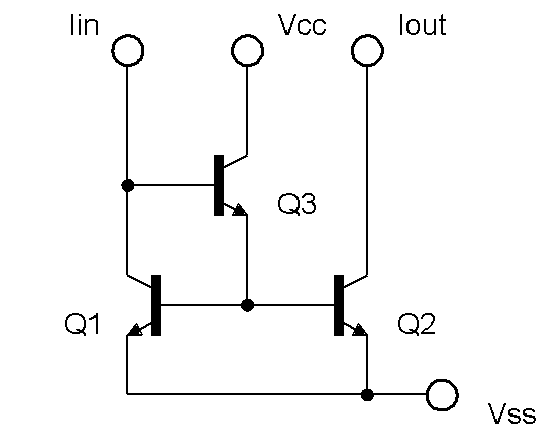
\includegraphics[scale=0.5]{obrazky/ZlepseneWilsonovoZrcadloNPN}
  \end{center}
  \caption[Alenčino zrcadlo]{Zlepšené Wilsonovo proudové zrcadlo.}
\end{figure}

Pro sazbu vektorových obrázků přímo v~\LaTeX{}u je možné doporučit balíček \href{https://www.ctan.org/pkg/pgf}{\texttt{TikZ}}.
Příklady sazby je možné najít na \href{http://www.texample.net/tikz/examples/}{\TeX{}ample}.
Pro vyzkoušení je možné použít programy QTikz nebo TikzEdt.




\chapter{Příklad sazby zdrojových kódů}

\section{Balíček \texttt{listings}}

Pro vysázení zdrojových souborů je možné použít balíček \href{https://www.ctan.org/pkg/listings}{\texttt{listings}}.
Balíček zavádí nové prostředí \texttt{lstlisting} pro sazbu zdrojových kódů, jako například:
%
\begin{lstlisting}[language={[LaTeX]TeX}]
\section{Balíček lstlistings}
Pro vysázení zdrojových souborů je možné použít
	balíček \href{https://www.ctan.org/pkg/listings}%
	{\texttt{listings}}.
Balíček zavádí nové prostředí \texttt{lstlisting} pro
	sazbu zdrojových kódů.
\end{lstlisting}
%
Podporuje množství programovacích jazyků.
Kód k~vysázení může být načítán přímo ze zdrojových souborů.
Umožňuje vkládat čísla řádků nebo vypisovat jen vybrané úseky kódu.
Např.:

\noindent
Zkratky jsou sázeny v~prostředí \texttt{acronym}:
\label{lst:zkratky}
\lstinputlisting[language={[LaTeX]TeX},nolol,numbers=left, firstnumber=6, firstline=6,lastline=6]{text/zkratky.tex}
%
Šířka textu volitelného parametru \verb|KolikMista| udává šířku prvního sloupce se zkratkami.
Proto by měla být zadávána nejdelší zkratka nebo symbol.
Příklad definice zkratky \acs{symfvz} je na výpisu \ref{lst:symfvz}.

\shorthandoff{-}
\lstinputlisting[language={[LaTeX]TeX},frame=single,caption={Ukázka sazby zkratek},label=lst:symfvz,numbers=left,linerange={bsymfvz-\%\%\%\ esymfvz},includerangemarker=false]{text/zkratky.tex}
\shorthandon{-}

\noindent
Ukončení seznamu je provedeno ukončením prostředí:
\lstinputlisting[language={[LaTeX]TeX},nolol,numbers=left,firstnumber=26,linerange=26]{text/zkratky.tex}

\vspace{\fill}

\noindent
{\bf Poznámka k~výpisům s~použitím volby jazyka \verb|czech| nebo \verb|slovak|:}\newline
Pokud Váš zdrojový kód obsahuje znak spojovníku \verb|-|, pak překlad může skončit chybou.
Ta je způsobená tím, že znak \verb|-| je v~českém nebo slovenském nastavení balíčku \verb|babel| tzv.\ aktivním znakem.
Přepněte znak \verb|-| na neaktivní příkazem \verb|\shorthandoff{-}| těsně před výpisem a hned za ním jej vraťte na aktivní příkazem \verb|\shorthandon{-}|.
Podobně jako to je ukázáno ve zdrojovém kódu šablony.


\clearpage

%\section{Výpis kódu prostředí Matlab}
Na výpisu \ref{lst:priklad.vypis.kodu.Matlab} naleznete příklad kódu pro Matlab, na výpisu \ref{lst:priklad.vypis.kodu.C} zase pro jazyk~C.

\lstnewenvironment{matlab}[1][]{%
\iflanguage{czech}{\shorthandoff{-}}{}%
\iflanguage{slovak}{\shorthandoff{-}}{}%
\lstset{language=Matlab,numbers=left,#1}%
}{%
\iflanguage{slovak}{\shorthandon{-}}{}%
\iflanguage{czech}{\shorthandon{-}}{}%
}

\begin{matlab}[frame=single,float=htbp,caption={Příklad Schur-Cohnova testu stability v~prostředí Matlab.},label=lst:priklad.vypis.kodu.Matlab,numberstyle=\scriptsize, numbersep=7pt]
%% Priklad testovani stability filtru

% koeficienty polynomu ve jmenovateli
a = [ 5, 11.2, 5.44, -0.384, -2.3552, -1.2288];
disp( 'Polynom:'); disp(poly2str( a, 'z'))

disp('Kontrola pomoci korenu polynomu:');
zx = roots( a);
if( all( abs( zx) < 1))
    disp('System je stabilni')
else
    disp('System je nestabilni nebo na mezi stability');
end

disp(' '); disp('Kontrola pomoci Schur-Cohn:');
ma = zeros( length(a)-1,length(a));
ma(1,:) = a/a(1);
for( k = 1:length(a)-2)
    aa = ma(k,1:end-k+1);
    bb = fliplr( aa);
    ma(k+1,1:end-k+1) = (aa-aa(end)*bb)/(1-aa(end)^2);
end

if( all( abs( diag( ma.'))))
    disp('System je stabilni')
else
    disp('System je nestabilni nebo na mezi stability');
end
\end{matlab}

\noindent
\begin{minipage}{\linewidth}


%\section{Výpis kódu jazyka C}

\begin{lstlisting}[frame=single,numbers=right,caption={Příklad implementace první kanonické formy v~jazyce C.},label=lst:priklad.vypis.kodu.C,basicstyle=\ttfamily\small, keywordstyle=\color{black}\bfseries\underbar,]
// první kanonická forma
short fxdf2t( short coef[][5], short sample)
{
	static int v1[SECTIONS] = {0,0},v2[SECTIONS] = {0,0};
	int x, y, accu;
	short k;

	x = sample;
	for( k = 0; k < SECTIONS; k++){
		accu = v1[k] >> 1;
		y = _sadd( accu, _smpy( coef[k][0], x));
		y = _sshl(y, 1) >> 16;

		accu = v2[k] >> 1;
		accu = _sadd( accu, _smpy( coef[k][1], x));
		accu = _sadd( accu, _smpy( coef[k][2], y));
		v1[k] = _sshl( accu, 1);

		accu = _smpy( coef[k][3], x);
		accu = _sadd( accu, _smpy( coef[k][4], y));
		v2[k] = _sshl( accu, 1);

		x = y;
	}
	return( y);
}
\end{lstlisting}
\end{minipage}







\chapter{Obsah elektronické přílohy}
Elektronická příloha je často nedílnou součástí semestrální nebo závěrečné práce.
Vkládá se do informačního systému VUT v~Brně ve vhodném formátu (ZIP, PDF\,\dots).

Nezapomeňte uvést, co čtenář v~této příloze najde.
Je vhodné okomentovat obsah každého adresáře, specifikovat, který soubor obsahuje důležitá nastavení, který soubor je určen ke spuštění, uvést nastavení kompilátoru atd.
Také je dobře napsat, v~jaké verzi software byl kód testován (např.\ Matlab 2018b).
Pokud bylo cílem práce vytvořit hardwarové zařízení,
musí elektronická příloha obsahovat veškeré podklady pro výrobu (např.\ soubory s~návrhem DPS v~Eagle).

Pokud je souborů hodně a jsou organizovány ve více složkách, je možné pro výpis adresářové struktury použít balíček \href{https://www.ctan.org/pkg/dirtree}{\texttt{dirtree}}.

\bigskip

{\small
%
\dirtree{%.
.1 /\DTcomment{kořenový adresář přiloženého archivu}.
.2 logo\DTcomment{loga školy a fakulty}.
.3 BUT\_abbreviation\_color\_PANTONE\_EN.pdf.
.3 BUT\_color\_PANTONE\_EN.pdf.
.3 FEEC\_abbreviation\_color\_PANTONE\_EN.pdf.
.3 FEKT\_zkratka\_barevne\_PANTONE\_CZ.pdf.
.3 UTKO\_color\_PANTONE\_CZ.pdf.
.3 UTKO\_color\_PANTONE\_EN.pdf.
.3 VUT\_barevne\_PANTONE\_CZ.pdf.
.3 VUT\_symbol\_barevne\_PANTONE\_CZ.pdf.
.3 VUT\_zkratka\_barevne\_PANTONE\_CZ.pdf.
.2 obrazky\DTcomment{ostatní obrázky}.
.3 soucastky.png.
.3 spoje.png.
.3 ZlepseneWilsonovoZrcadloNPN.png.
.3 ZlepseneWilsonovoZrcadloPNP.png.
.2 pdf\DTcomment{pdf stránky generované informačním systémem}.
.3 student-desky.pdf.
.3 student-titulka.pdf.
.3 student-zadani.pdf.
.2 text\DTcomment{zdrojové textové soubory}.
.3 literatura.tex.
.3 prilohy.tex.
.3 reseni.tex.
.3 uvod.tex.
.3 vysledky.tex.
.3 zaver.tex.
.3 zkratky.tex.
%.2 navod-sablona\_FEKT.pdf\DTcomment{návod na používání šablony}.
.2 sablona-obhaj.tex\DTcomment{hlavní soubor pro sazbu prezentace k~obhajobě}.
%.2 readme.txt\DTcomment{soubor s~popisem obsahu CD}.
.2 sablona-prace.tex\DTcomment{hlavní soubor pro sazbu kvalifikační práce}.
.2 thesis.sty\DTcomment{balíček pro sazbu kvalifikačních prací}.
}
}


\end{document}
